\chapter{Learning data from a resolved liquid jet in crossflow}
	\label{ch5:jicf_resolved_simulations}



Describe here all our simulations done with JICF, what we have achieved with them, etc.

\begin{itemize}

	\item Experimental setup description
	
	\item Numerical setup description. Operating points
	
	\item Mesh convergence study
	
	\item Spray sampling
	
	\item Direct measurement of fluxes with interior boundaries
	
	\item Liquid disappearing (set levelset band ) ??
	
	\item Results:
	
		\begin{itemize}
		
			\item Breakup mechanisms
			
			\item In-nozzle phenomena of flow separation (and entrainment of gaseous bubbles)
			
			\item Spray formation and evolution with axial distance
	
		\end{itemize}
		
	\item Other results:
	
		\begin{itemize}
		
			\item Slip velocity evolution
			
			\item Vorticity distribution (horse-shoe vortices, double vortical structural in liquid)
		
		\end{itemize}

\end{itemize}

\newpage 

\section{Introduction}

The previous chapter has detailed the theory of the proposed models to build lagrangian injectors for initialising dispersed phase simulations, named Smart Lagrangian Injectors (SLI). These models, nowadays in its earliest state of maturity, are intended to be generic and applicable to a broad range of operating conditions and injector configurations. To show its capabilities, they have been developed in their first stage with resolved simulations of liquid jet in crossflow (JICF) configuration. This chapter details these simulations, performed with the software YALES2 \citepColor[moureau_design_2011]. % \textbf{https://reader.elsevier.com/reader/sd/pii/S1631072110002111?token=9137B6903478D4E8E427F5D8218DFC3EB42446DB034970B14BA9DE87AA7E80D130124A7EF8D8608D21D5D465CCE05A4F&originRegion=eu-west-1&originCreation=20210524114835}

The fundamentals and the physics of non-reactive JICF have been introduced in $\S$\ref{sec:ch1_fuel_injection_technology}. This chapter shows the results, analysis and injectors obtained from a kerosene JICF simulation replicating the experimental facility tested by \citeColor[becker_breakup_2002]. This configuration is used for validating the models. Section \ref{sec:ch5_experimental_bench} displays the experimental test bench, whose numerical setup and operating conditions chosen for numerical computations are detailed in Section \ref{sec:computational_setup}.


\section{Experimental test case}
	\label{sec:ch5_experimental_bench}

The experimental configuration tested by \citeColor[becker_breakup_2002] is shown in Figure \ref{fig:experiment_JICF_DLR}. The test rig is shown at the left. Liquid kerosene is injected through the atomizer ports to a quartz glass duct of rectangular cross section $25$x$40$ mm$^2$. The duct inlet is located at $120$ mm upstream the injection port. The boundary layer thickness developing along the bottom of the duct has been measured experimentally just upstream the atomizer, being between $4$ and $5$ mm. The lateral walls allow for optical access from the atomizer port until a location at 100 mm downstream. Air is introduced through two separate channels, a main one and a supplementary one. The main airflow is injected at the inlet of the quartz duct, while the supplementary one passes around it. Both airflows merge at the end of the duct and leave the domain through a common exit acting as a sonic throttle. The velocity inside the quartz can then be tuned by varying the size of the nozzle and the supplementary air flow rate. In the experiments performed, the range of air velocities goes from $u_g = 50$ to 100 m/s and the range of pressure from $p$ = 1.5 to 15 bar, hence allowing the study high-pressure conditions. The air temperature is maintained to $T_g = 290$ K. The fuel tested was kerosene Jet A-1 with density $\rho_l = 795$ kg m$^{-3}$ and surface tension $\sigma = 22 \cdot 10^{-3}$ N m$^{-1}$.

The liquid injection nozzle can be seen in Figure \ref{fig:experiment_JICF_DLR} right. It consists of a plain jet nozzle of $d_\mathrm{inj} =  0.45$ mm diameter and $L/d_\mathrm{inj}$ ratio of 1.56 with sharp edges. The average discharge coefficient for the mass flow rates of interest in the experimental studies is $0.6$. More details on the test rig can be found in \citeColor[brandt_experimental_1997].

\begin{figure}[h!]
	\centering
	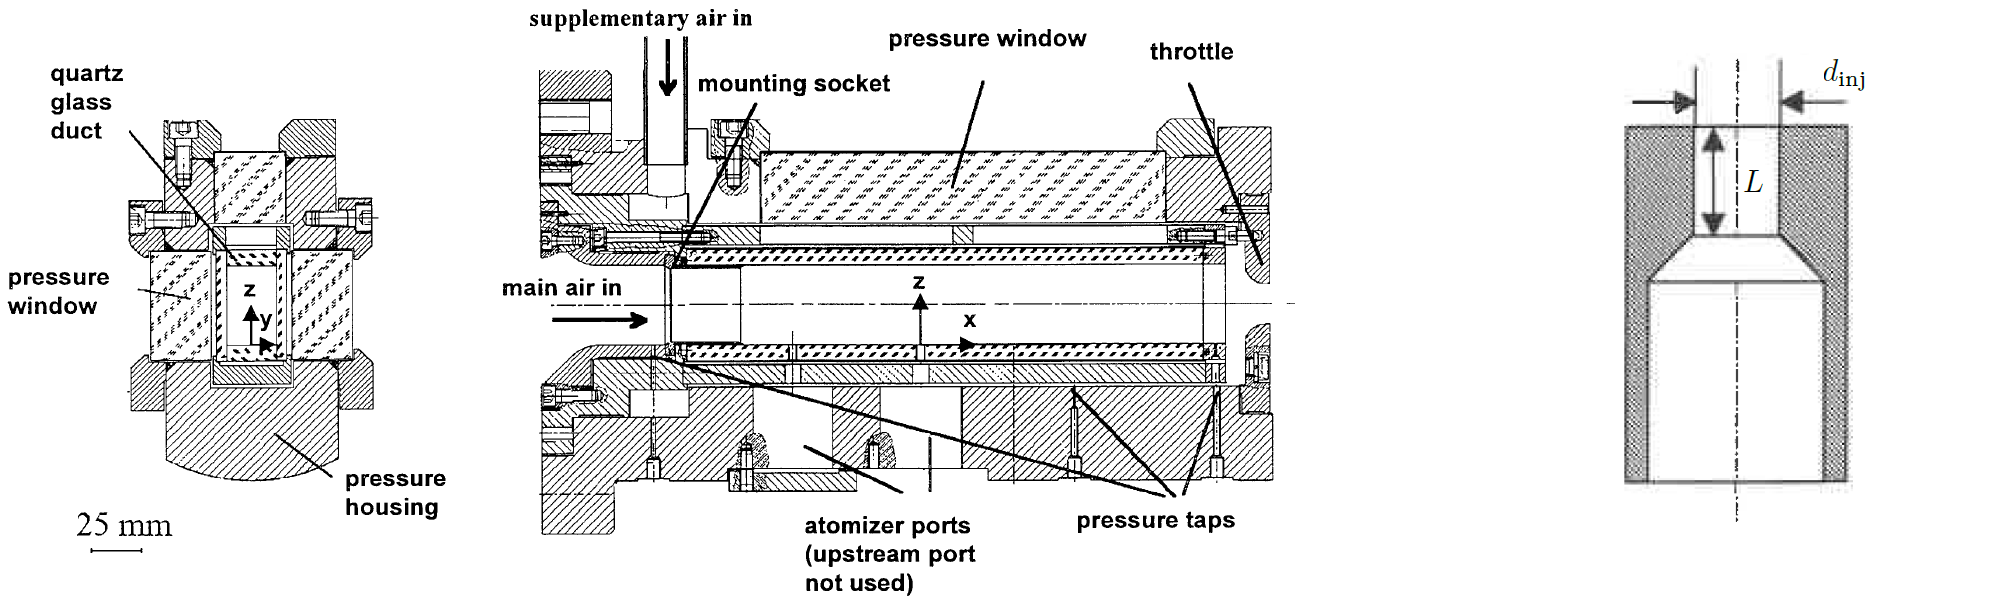
\includegraphics[scale=0.35]{./part2_developments/figures_ch5_resolved_JICF/experiment_JICF_DLR}
	\caption[JICF experimental setup]{JICF experimental setup. \textsl{Left}: Test rig. \textsl{Right}: liquid nozzle geometry employed in the experimental study. Source: \citeColor[becker_breakup_2002]}
	\label{fig:experiment_JICF_DLR}
\end{figure}


A correlation for the trajectory of the jet was obtained experimentally by analysing optically its penetration for the several operating conditions tested. It corresponds to the trajectory of the jet's windward side, and gives a relation between the vertical location $z$ with respect to the axial coordinate $z$ as a function of the nozzle diameter $d_\mathrm{inj}$ and the momentum ratio $q$ defined by Eq. (\ref{eq:q_and_We_JICF_parameters}): % The rorrelation has a standard deviation of 0.81.

\begin{equation}
    \label{eq:jicf_trajectory_becker}
    \frac{z}{d_\mathrm{inj}} = 1.57 \mathrm{q}^{0.36} \ln \left( 1 + 3.81 \frac{x}{d_\mathrm{inj}} \right)
\end{equation}



\section{Computational setup}
	\label{sec:computational_setup}

%\subsection*{Numerical domain and baseline mesh}

Figure \ref{fig:numerical_setup_maquette_JICF_DLR} shows the computational domain developed to replicate the simulations of the test bench shown in Figure \ref{fig:experiment_JICF_DLR}. The duct is modelled as a plenum consisting of a box of dimensions 25x40x270 mm$^3$. The hydraulic diameter of the duct cross section, which is used to calculate the gas Reynolds number, is $D_h = 30.8$ mm. A magnified view of the nozzle is also shown, with diameter $0.45$ mm and straight section length of 0.7 mm prior to injection to keep $L/D = 1.56$ as in the experiments. The boundary conditions are also indicated. The plenum walls use a wall law of logarithmic type except closer to the domain pressure outlet, which have been set to slip walls to avoid backflow. The nozzle walls are rigid walls. For the liquid inlet, a Poiseuille profile has been specified, while in the gaseous inlet a mean velocity profile has been set in order to recover the boundary layer thickness of between 4 and 5 mm upstream the injection nozzle as described in the experiments (see Appendix \ref{app:JICF_BL_setup} for details). Due to the high Reynolds number at the gaseous inlet (see Table \ref{tab:jicf_operating_conditions}), synthetic turbulence is added in the liquid inlet (details given in $\S$\ref{sec:ch5_initial_conditions}).

\begin{figure}[ht]
     \centering
     \includeinkscape[scale=0.35]{./part2_developments/figures_ch5_resolved_JICF/DLR_becker_numerical_config}
      \caption{Numerical domain and boundary conditions of the experimental test bench of \citeColor[becker_breakup_2002]. \textsl{Left}: complete domain. \textsl{Right}: detailed view of the injection nozzle. All dimensions are in mm.}
      \label{fig:numerical_setup_maquette_JICF_DLR}
\end{figure}

%Figure \ref{fig:jicf_dlr_mesh} shows the baseline mesh, where the symmetry plane at $y = 0$ is displayed. It is composed of 66 million tetrahedral cells. The baseline cell size in the channel upstream liquid injection is 0.5 mm, while the cells located in the downstream region have an average size of 3 mm. The element size at the near-field region is 0.7 mm, and within the discharge section of the liquid nozzle it is refined to to $20~\mu m$. The justification of this mesh is done at $\S$\ref{sec:ch5_initial_conditions}, where a mesh independence study of the gaseous field is carried out. This mesh is used at the beginning of all the simulations performed, but then it change dynamically in each simulation as more liquid is introduced in the domain due to the AMR routine that refines the mesh at the liquid-gas interface ($\S$\ref{sec:YALES2}). Simulations are performed with the ACLS methodology describe in $\S$\ref{subsec:ch2_ACLS}.

Figure \ref{fig:jicf_dlr_mesh} shows the baseline mesh, where the symmetry plane at $y = 0$ is displayed. It is composed of 66 million tetrahedral cells. The baseline cell size in the channel upstream liquid injection is 0.5 mm, while the cells located in the downstream region have an average size of 3 mm. The element size within the discharge section of the liquid nozzle it is refined to to $20~\mu m$. The justification for this mesh choice is done at $\S$\ref{sec:ch5_initial_conditions}, where a mesh independence study of the gaseous field is carried out. This mesh is used at the beginning of all the simulations performed, but then it change dynamically in each simulation as more liquid is introduced in the domain due to the AMR routine that refines the mesh at the liquid-gas interface ($\S$\ref{sec:YALES2}). Simulations are performed with the ACLS methodology describe in $\S$\ref{subsec:ch2_ACLS}.

\begin{figure}[h!]
	\centering
	\includeinkscape[inkscapelatex=false,scale=0.7]{./part2_developments/figures_ch5_resolved_JICF/jicf_mesh/jicf_mesh}
	\caption[Baseline JICF mesh, showing magnified views of the near-field and nozzle regions.]{Baseline JICF mesh, showing magnified views of the near-field and nozzle regions. The red rectangle is the region where meshes are shown in the mesh convergence study of $\S$\ref{sec:ch5_initial_conditions}}
	\label{fig:jicf_dlr_mesh}
\end{figure}



\section{Operating conditions}

Two operating conditions tested experimentally in \citeColor[becker_breakup_2002] have been simulated. Both of them have the same momentum ration $q = 6$ but differ in the Weber number: $We_g = 830$ (low Weber) and $We_g = 1470$ (low Weber). According to the values of $q$ and $We_g$, the former condition corresponds to surface breakup dominating regime while the latter is located at the dividing line between column and surface breakup. Figure \ref{fig:location_JICF_ops_in_breakup_map} shows the location of both operating points in the breakup map of \citeColor[wu_breakup_1997]. The physical magnitudes and dimensionless numbers of both operating points are shown in Table \ref{tab:jicf_operating_conditions}. Apart from the values $q$ and $We_g$, the dimensionless numbers in  Eq. (\ref{eq:dimensionless_numbers_jicf}) are also calculated: the liquid and gaseous Reynolds numbers $Re_g$ and $Re_g$ respectively, Ohnesorge number $Oh$, aerodynamic Weber $We_\mathrm{aero}$, relative Weber $We_\mathrm{rel}$ and density ratio $r$. These numbers have been added since they are defined in several experimental studies \citeColor[wu_breakup_1997,becker_breakup_2002,ragucci_trajectory_2007] to characterize the operating points tested. 

For performing the computations of resolved atomization, the ACLS methodology combined with the AMR routine described in $\S$\ref{subsec:ch2_ACLS} is used. For each simulation, two interface mesh sizes have been simulated: $\Delta x_\mathrm{min} = 20 ~\mu m$ (coarse case) and $\Delta x_\mathrm{min} = 10 ~\mu m$ (fine case). Therefore, a total of four simulations have been done. The nomenclature for each simulation, which is used hereafter in this document, is introduced in Table \ref{tab:jicf_resolved_simulations_performed}.

%\begin{subequations}
%\label{eq:dimensionless_numbers_jicf}
%\begin{align}
%Re_l &= \frac{\rho_l u_l d_\mathrm{inj}}{\mu_l}\\
%Re_g &= \frac{\rho_g u_g D_h}{\mu_g}\\
%We_\mathrm{aero} &= \frac{\rho_g u_l^2 d_\mathrm{inj}}{\sigma}  \\
%We_\mathrm{rel} &= \frac{\rho_g \left( u_g - u_l \right)^2 d_\mathrm{inj}}{\sigma} \\
%Oh &=  \frac{\mu_l}{\sqrt{\rho_l \sigma d_\mathrm{inj}}}\\
%r &= \frac{\rho_l}{\rho_g} 
%\end{align}
%\end{subequations}

%\begin{align}
%\label{eq:dimensionless_numbers_jicf}
%Re_l &= \frac{\rho_l u_l d_\mathrm{inj}}{\mu_l}          &  Re_g &= \frac{\rho_g u_g D_h}{\mu_g}              &  Oh &=  \frac{\mu_l}{\sqrt{\rho_l \sigma d_\mathrm{inj}}}\\
%We_\mathrm{aero} &= \frac{\rho_g u_l^2 d_\mathrm{inj}}{\sigma}    &  We_\mathrm{rel} &= \frac{\rho_g \left( u_g - u_l \right)^2 d_\mathrm{inj}}{\sigma}          & r &= \frac{\rho_l}{\rho_g} 
%\end{align}


\begin{equation}
\label{eq:dimensionless_numbers_jicf}
\begin{aligned}
Re_l &= \frac{\rho_l u_l d_\mathrm{inj}}{\mu_l}          &  Re_g &= \frac{\rho_g u_g D_h}{\mu_g}              &  Oh &=  \frac{\mu_l}{\sqrt{\rho_l \sigma d_\mathrm{inj}}}\\
We_\mathrm{aero} &= \frac{\rho_g u_l^2 d_\mathrm{inj}}{\sigma}    &  We_\mathrm{rel} &= \frac{\rho_g \left( u_g - u_l \right)^2 d_\mathrm{inj}}{\sigma}          & r &= \frac{\rho_l}{\rho_g} 
\end{aligned}
\end{equation}

\begin{table}[!h]
\centering
\caption{JICF operating points studied}
\begin{tabular}{lcccc}
\thickhline
\textbf{Parameter} & \textbf{Symbol} & \textbf{Units} &  \textbf{Low Weber} &  \textbf{High Weber} \\ %\textbf{WE\_880} &  \textbf{WE\_1470} \\
\thickhline
Nozzle diameter & $d_\mathrm{inj}$ & mm & 0.45 & 0.45 \\
%\hline
Gas bulk velocity & $u_g$ & m s$^{-1}$ & 75 & 100 \\
%\hline
Gas flow rate & $Q_g$ & m$^3$ s$^{-1}$ & 0.075  & 0.1 \\
%\hline
Liquid bulk velocity & $u_l$ & m s$^{-1}$ & 17.5  & 23.33 \\
%\hline
Liquid flow rate & $Q_l$ & mm$^3$ s$^{-1}$ & 2783  & 3710 \\
%\hline
Ambient pressure & $p_\mathrm{amb}$ & bar &  6 & 6 \\
%\hline
Gas temperature & $T_g$ & K & 290 & 290 \\
%\hline
Liquid temperature & $T_l$ & K & 290 & 290 \\
%\hline
Gas density & $\rho_g$ & kg m$^{-3}$ &  7.21 & 7.21 \\
%\hline
Liquid density & $\rho_l$ & kg m$^{-3}$ &  795 & 795  \\
%\hline
Gas viscosity & $\mu_g$ & kg m$^{-1}$ s$^{-1}$ & $1.8162 \cdot 10^{-5}$ &  $1.8162 \cdot 10^{-5}$  \\
%\hline
Liquid viscosity & $\mu_l$ & kg m$^{-1}$ s$^{-1}$ & $1.5 \cdot 10^{-3}$ & $1.5 \cdot 10^{-3}$  \\
%\hline
Surface tension & $\sigma$ & kg s$^{-2}$ &  0.022 & 0.022  \\
\thickhline
Momentum ratio & $q$ & - & 6 & 6 \\
%\hline
Gas Reynolds number & $Re_g$ & - & $0.92 \cdot 10^6$ & $1.22 \cdot 10^6$ \\
%\hline
Liquid Reynolds number & $Re_l$ & - & 4170 & 5560 \\
%\hline
Gas Weber number & $We_g$ & - & 830 & 1470 \\
%\hline
Liquid Weber number & $We_l$ & - & 5000 & 8850 \\
%\hline
Relative Weber number & $We_\mathrm{rel}$ & - & 490 & 870 \\
%\hline
Aerodynamic Weber number & $We_\mathrm{aero}$ & - & 45 & 80 \\
%\hline
Ohnesorge number & $Oh $ & - & 0.017 & 0.017 \\
%\hline
Density ratio & $r$ & - & 110 & 110 \\
%\hline
%Viscosity ratio & $\mu_l/\mu_g$ & [-] &  \multicolumn{2}{|c|}{1} \\
\thickhline
\end{tabular}
\label{tab:jicf_operating_conditions}
\end{table}

\clearpage


\begin{table}[!h]
\centering
\caption{Nomenclature for resolved atomization simulations}
\begin{tabular}{ccc}
\thickhline
%$\pmb{\Delta} x_\mathrm{min}$ [$\pmb{\mu}$$\textbf{m}])  &  \multicolumn{2}{c}{\textbf{Operating condition}} \\ 
$\Delta x_\mathrm{min}$ [$\mu$m]  &  \multicolumn{2}{c}{\textbf{Operating condition}} \\ 
\cline{2-3}
 &  Low $We_g$ &  High $We_g$ \\ 
\thickhline
\textbf{10} & UG75\_DX10 & UG100\_DX10 \\
\textbf{20} & UG75\_DX20 & UG100\_DX20 \\
\thickhline
\end{tabular}
\label{tab:jicf_resolved_simulations_performed}
\end{table}

\begin{figure}[ht]
     \centering
     \includeinkscape[inkscapelatex=false,scale=0.6]{./part2_developments/figures_ch5_resolved_JICF/jicf_breakup_regime_our_operating_points}
     \caption{Location of simulated operating conditions in the breakup map by \citeColor[wu_breakup_1997]}
	% See: https://stackoverflow.com/questions/35210337/can-i-plot-several-histograms-in-3d/35225919
      \label{fig:location_JICF_ops_in_breakup_map}
\end{figure}



%\section{YALES2 code (??)}

\section{Tools and methodologies}

%\subsection{Spray sampling in resolved simulations}

\subsection{Numerical computation of jet trajectory}
	\label{sec:ch5_tools_jicf_trajectories}

One of the most important characteristics of a jet in crossflow is its trajectory (see $\S$\ref{sec:ch1_fuel_injection_technology}). This feature determines how far the jet penetrates in the domain and has a paramount effect on the latter evaporation and mixing processes, hence affecting the flame dynamics. Experimental studies often provide correlations for the trajectory of the windward side of the jet (see Table \ref{tab:correlations_experimental_JICF}), such as the one from Eq. (\ref{eq:jicf_trajectory_becker}). These correlations depend generally on the momentum flux ratio $q$, the injection diameter $d_\mathrm{inj}$ and, in some case \citepColor[ragucci_trajectory_2007], in the Weber number $We$. The overall dependency of the trajectory on these parameters is still unknown.

Experimentally, researches have used different approaches to obtain trajectories based on the different optical techniques employed. Many works \citemColor[becker_breakup_2002,stenzler_penetration_2003,freitag_spray_2008] obtain instantaneous images of the jet with shadowgraphy techniques and then MIE scattering or emboss-filter operations to obtain binary images where liquid and gas phases can be clearly distinguished. Then, images are averaged and the vertical penetration is obtained by detecting the coordinates where the light intensity gradients are maximum. The image averaging can be performed before or after the filtering operations. These methods, which are based on obtaining the trajectories from mean images, are hereafter denoted as \textbf{mean trajectory methods}. Figure \ref{fig:expe_obtention_of_trajectories} shows an illustration of such experimental methodology from the work by \citeColor[stenzler_penetration_2003]. The filtering operations and way to obtain the light gradients vary among authors. Other works \citepColor[ragucci_trajectory_2007] use the same principles of filtering and binarization, but obtain the trajectories from instantaneous jet images. Then, the instantaneous trajectories are averaged to yield the mean trajectories. These methods are hereafter denoted as \textbf{instantaneous trajectory methods}.

From a computational perspective, similar methodologies can be applied to obtain the jet trajectories from simulations. The same sequence of operations as shown in Figure \ref{fig:expe_obtention_of_trajectories} used to process experimental images could be applied to numerical snapshots of the JICF. Nevertheless, the ACLS methodology presents the advantage that the interface can be clearly defined with the $\psi$ function, and hence it can be used to obtain the trajectory by different methods. In this work, four methodologies to obtain the numerical trajectories from JICF resolved simulations are presented. As in the experimental classification previously suggested to obtain trajectories, these methodologies are also distinguished as \textbf{mean trajectory methods} or \textbf{instantaneous trajectory methods}, depending on whether they use the mean or instantaneous $\psi$ field respectively. Two methods for each category are detailed in this section, while the results obtained are shown in $\S$\ref{subsec:ch5_jet_trajectories_results}.

\begin{figure}[ht]
     \centering
     \includeinkscape[inkscapelatex=false,scale=0.6]{./part2_developments/figures_ch5_resolved_JICF/trajectories_obtention/expe_obtention}
     \caption{Illustration of experimental procedure to obtain trajectories. Figures taken from \citeColor[stenzler_penetration_2003]}
      \label{fig:expe_obtention_of_trajectories}
\end{figure}


\subsubsection{Instantaneous trajectory methods}

The averaged numerical trajectories can be obtained from instantaneous solutions of the jet by obtaining the instantaneous trajectories for every solution obtained and then averaging them. Figure \ref{fig:trajectory_obtention_instantaneous_general} shows the procedure to extract the interface contour that is later used to obtain the trajectories. First, the liquid-gas interface is plotted in the domain as a surface of iso-contour $\Gamma: \psi = 0.5$ (Figure \ref{fig:trajectory_obtention_instantaneous_general} left), and then this contour is extracted at the central plane $y = 0$, as indicated by the black line of Figure \ref{fig:trajectory_obtention_instantaneous_general} right. 

\begin{figure}[ht]
     \centering
     \begin{subfigure}[b]{0.45\textwidth}
         \centering
         \includeinkscape[inkscapelatex=false,scale=0.35]{./part2_developments/figures_ch5_resolved_JICF/trajectories_obtention/instantaneous_interface_3D}
         %\caption{Instantaneous jet interface}
     \end{subfigure}
     %\hfill
     \begin{subfigure}[b]{0.45\textwidth}
         \centering
         \includeinkscape[inkscapelatex=false,scale=0.35]{./part2_developments/figures_ch5_resolved_JICF/trajectories_obtention/instantaneous_interface_y0}
         %\caption{Contour of instantaneous interface at plane y = 0}
     \end{subfigure}
        \caption[Procedure to obtain instantaneous trajectories.]{Procedure to obtain instantaneous trajectories. \textsl{Left}: instantaneous jet interface. \textsl{Right}: contour of instantaneous interface at plane y = 0}
	% See: https://stackoverflow.com/questions/35210337/can-i-plot-several-histograms-in-3d/35225919
        \label{fig:trajectory_obtention_instantaneous_general}
\end{figure}

Once the interface is obtained at $y = 0$, the outer contour of the trajectory must be obtained. This is the one corresponding to the windward side of the jet, and hence the one defining the instantaneous trajectory. For its obtention, the $z$ axis is swept and the points belonging to the trajectory are obtained as follows:

\begin{enumerate}

	\item The $z$ axis is discretized in intervals with thickness $\Delta z$. 
	
	\item For each interval, the contour point with minimum $x$ coordinate is obtained.
	
	\item Points are sorted according to their $x$ coordinate, defining the trajectory.

\end{enumerate}

This procedure is repeated at every instantaneous snapshot of the jet to obtain the instantaneous trajectories. Then, all the trajectories obtained are interpolated to obtain the mean trajectories which can be compared to experimental correlations. This method is similar to the experimental methodology employed by \citeColor[ragucci_trajectory_2007] to obtain mean trajectories, and was used by \citeColor[leparoux_primary_2018] to simulate their experimental configuration and compare numerical trajectories with experiments. However, it differs from the methodology employed by \citeColor[becker_breakup_2002], whose experimental test rig is simulated in this work and who obtain the trajectories with a methodology more similar to the mean trajectory methods (see next point). Still, it is worth to investigate the instantaneous methodologies to obtain the trajectories and to compare them with the mean methods.

The procedure previously described works properly in the dense core, where the interface contour is continuous up to the breakup point $z_b$. After this location, atomization takes place and the detected $\Gamma$ contours belong to ligaments or droplets. In this case, the definition of \textsl{outer trajectory} does not hold as clearly as in the dense core: some contours detected might belong to satellite droplets or to drops originated from surface breakup, and could modify the final average trajectory by lowering it down. With this consideration, two different trajectories are distinguished in the instantaneous methodologies: \textbf{non-monotonic} and \textbf{monotonic} trajectories. These are discussed in the following lines.

%\subsubsection*{Non-monotonic trajectory}

\paragraph*{{Non-monotonic trajectory}} 

Non-monotonic instantaneous trajectories can be obtained by applying the methodology as explained in the previous lines, accounting also for the contours which a priori do not pertain to the outer contour of the instantaneous trajectory. This procedure is illustrated in Figure \ref{fig:trajectory_obtention_instantaneous_method_a}: the different points of the trajectory are obtained when sweeping the $z$ axis, and the instantaneous trajectory is obtained by joining these points. Then, sorting all the sampled points along the $x$ axis creates a non-monotonic trajectory since some contour points belong to liquid structures further downstream, see Figure \ref{fig:trajectory_obtention_instantaneous_method_a} right.

\begin{figure}[ht]
     \centering
     \begin{subfigure}[b]{0.45\textwidth}
         \centering
         \includeinkscape[inkscapelatex=false,scale=0.35]{./part2_developments/figures_ch5_resolved_JICF/trajectories_obtention/method_a_sweep_nonMonotonic}
         %\caption{Instantaneous jet interface}
     \end{subfigure}
     %\hfill
     \begin{subfigure}[b]{0.45\textwidth}
         \centering
         \includeinkscape[inkscapelatex=false,scale=0.34]{./part2_developments/figures_ch5_resolved_JICF/trajectories_obtention/method_a_inst_trajectory}
         %\caption{Contour of instantaneous interface at plane y = 0}
     \end{subfigure}
        \caption[Obtention of non-monotonic instantaneous trajectory]{Obtention of non-monotonic instantaneous trajectory. \textsl{Left}: sweep process along z axis of interface points. \textsl{Right}: instantaneous trajectory.}
	% See: https://stackoverflow.com/questions/35210337/can-i-plot-several-histograms-in-3d/35225919
        \label{fig:trajectory_obtention_instantaneous_method_a}
\end{figure}


\clearpage

%\subsubsection*{Monotonic trajectory}
\paragraph*{Monotonic trajectory} 

The procedure is identical to the obtention of non-monotonic trajectories with one fundamental difference: when sorting along the $x$ axis, only points with increasing $z$ coordinate are considered. In this way, a monotonic trajectory is obtained, see Figure \ref{fig:trajectory_obtention_instantaneous_method_b} right. 


\begin{figure}[ht]
     \centering
     \begin{subfigure}[b]{0.45\textwidth}
         \centering
         \includeinkscape[inkscapelatex=false,scale=0.35]{./part2_developments/figures_ch5_resolved_JICF/trajectories_obtention/method_b_sweep_monotonic}
         %\caption{Instantaneous jet interface}
     \end{subfigure}
     %\hfill
     \begin{subfigure}[b]{0.45\textwidth}
         \centering
         \includeinkscape[inkscapelatex=false,scale=0.33]{./part2_developments/figures_ch5_resolved_JICF/trajectories_obtention/method_b_inst_trajectory}
         %\caption{Contour of instantaneous interface at plane y = 0}
     \end{subfigure}
        \caption[Obtention of monotonic instantaneous trajectory]{Obtention of monotonic instantaneous trajectory. \textsl{Left}: sweep process along z axis of interface points, excluding points whose vertical location is lower than the vertical location of the previous ones. \textsl{Right}: instantaneous trajectory.}
	% See: https://stackoverflow.com/questions/35210337/can-i-plot-several-histograms-in-3d/35225919
        \label{fig:trajectory_obtention_instantaneous_method_b}
\end{figure}

The two instantaneous methodologies described here will provide the same trajectories in the dense core, but will differ after the breakup point. Therefore, the trajectories obtained from this methodology can be compared and used to estimate an average position of the dense core. 


\subsubsection{Mean trajectory methods}

Another possibility to obtain mean trajectories is by using the mean field of the levelset function, $\overline{\psi}$. An example of a converged $\overline{\psi}$ field is shown in Figure \ref{fig:trajectory_obtention_mean_methods_c_d} left.. This requires the accumulation of statistics over a certain time (instantaneous trajectories do not need accumulation statistics as long as the instantaneous $\psi$ field is available), but presents the advantage that the jet trajectory can be obtained with one single $\overline{\psi}$ field once convergence is achieved. In this category, two different methods are used: the \textbf{maximum gradient method} and the \textbf{iso-contour method}.

\begin{figure}[ht]
     \centering
     \includeinkscape[inkscapelatex=false,scale=0.35]{./part2_developments/figures_ch5_resolved_JICF/trajectories_obtention/methods_c_d_and_mean_psi_field}
     \caption[Methods based on mean trajectories]{Methods based on mean trajectories. \textsl{Left}: $\overline{\psi}$ field. \textbf{Center}: $\max \left( \nabla_z | \overline{\psi} | \right)$ contour. \textsl{Right}: contour $\overline{\psi} = 0.01$.}
	% See: https://stackoverflow.com/questions/35210337/can-i-plot-several-histograms-in-3d/35225919
      \label{fig:trajectory_obtention_mean_methods_c_d}
\end{figure}



\paragraph{Maximum gradient method}

This method is more similar to the experimental methods presented in \citeColor[becker_breakup_2002], \citeColor[stenzler_penetration_2003] and \citeColor[freitag_spray_2008]. In these works, the jet trajectory is obtained as the contour of the maximum intensity gradient in the vertical direction of the mean jet (see Figure \ref{fig:expe_obtention_of_trajectories}). In a similar fashion, an equivalent postprocessing can be performed in the computations by obtaining the maximum gradient of $\overline{\psi}$ in the vertical direction for each $x$ coordinate: $\max \left( \nabla_z | \overline{\psi} | \right)$. The absolute value of $\overline{\psi}$ is taken because the interest is to retrieve the outer contour where $\overline{\psi}$ decreases along the vertical direction from $1$ (liquid) to 0 (gas), so the gradient is negative. Figure \ref{fig:trajectory_obtention_mean_methods_c_d} center shows an example of a $\max \left( \nabla_z | \overline{\psi} | \right)$ contour. \\


\paragraph{Trajectory as iso-contour of mean $\overline{\psi}$}

A more intuitive methodology is to obtain the trajectory as an iso-contour of the mean levelset field $\overline{\psi}$. This approach has been used to obtain JICF trajectories with simulations using a VOF methodology \citepColor[desclaux_experimental_2020]. In this works, several values for the iso-contour have been tested, and it has been found that the mean trajectories obtained are very sensitive to this value. Finally, a value of $\overline{\psi} = 0.01$ has been identified as the best contour to compare the resulting trajectories with the ones obtained with the rest of methods. Figure \ref{fig:trajectory_obtention_mean_methods_c_d} right shows an example of a an example of a $\overline{\psi} = 0.01$ contour. \\

Table \ref{tab:jicf_tools_trajectories_obtention} shows a summary of the four methodologies presented, and the names used in $\S$\ref{subsec:ch5_jet_trajectories_results} to display the results.

\begin{table}[!h]
\centering
\caption{Summary of methods for computing JICF trajectories}
\begin{tabular}{ccc}
\thickhline
Group & Method & Name \\
\thickhline
\multirow{2}{*}{Instantaneous} & Non-monotonic & INST\_NM \\
 & Monotonic & INST\_M \\
 \hline
\multirow{2}{*}{Mean} & Maximum gradient & MEAN\_GRAD \\
 & Iso-contour & MEAN\_CONT \\
\thickhline
\end{tabular}
\label{tab:jicf_tools_trajectories_obtention}
\end{table}

\subsection{Direct measurement of liquid fluxes}
\label{subsec:ch5_interior_boundaries}

Droplet sampling procedure, described in $\S$\ref{subsec:SLI_spray_sampling}, is performed by tracking the center of mass of resolved structures and sampling the droplets when they cross the defined sampling planes by lagrangian projection. With this procedure, some droplets are tracked twice and some others might never be tracked. As a consequence, the sampled spray is not actually the \textsl{true} spray that crosses the sampling surfaces in the simulations, but an approximation to it. Therefore, the obtained spray size distributions and sampled mass flow rates are also affected.

In order to check the accuracy of the lagrangian projection procedure for tracking droplets, the mass flow rates are compared to flow rates measured directly in the resolved simulations. The direct measurement of liquid fluxes is performed by defining \textbf{interior boundaries} (IBs) in the sampling surfaces. IBs are formed by all the mesh elements contained in the surface, and liquid flow rates can be calculated by applying directly Eq. (\ref{eq:mass_flow_rate_definition_general}) divided by the density, with $\phi = \psi$ being the levelset function:

\begin{equation}
\label{eq:Q_lIB_general_definition}
Q_{l,\mathrm{IB}} = \int_{\mathrm{IB}} \psi \left( \textbf{u} \cdot \textbf{n} \right) dS
\end{equation}

Figure \ref{fig:jicf_interior_boundaries_surface_measurements} shows an example of IBs located in a JICF simulation. Four IBs are defined in sampling planes perpendicular to the crossflow equally spaced at a distance of 5 mm: $x = 5, 10, 15$ mm. These IBs match the sampling planes where spray is sampled, so that fluxes can be directly compared. Furthermore, four more sampling planes parallel to the wall to quantify the liquid flow rate that impinges the wall, known as filming: $x <5, 10, 15$ mm. Therefore, each combination of sampling and filming IB will conform the outlet surfaces of a control volume enclosing the whole liquid jet (no outlet surfaces are located upstream the injection point as there is no liquid flowing in this direction). The inlet surface corresponds to the liquid nozzle.



In order to apply Eq. (\ref{eq:Q_lIB_general_definition}), the fluxes need to be calculated at each IB element and then be added. Figure \ref{fig:jicf_IBs_sketch_calculation} shows an example of IB composed by the mesh elements, and shows a zoom-in view of a single plane element. $e$ Each element is defined by a normal $n_e$ and by three nodes $N_\mathrm{no} = 3$, since the mesh used is tetrahedral. Simulation data is stored at the nodes, so the instantaneous liquid flux passing through each single element can be calculated as:

\begin{equation}
Q_{l,e} = \frac{1}{N_\mathrm{no}} \sum_{i=1}^{N_\mathrm{no}} \psi_i \textbf{u}_i \textbf{n}_e
\end{equation}

Then, the total flux in the IB is obtained by applying Eq. (\ref{eq:Q_lIB_general_definition}) in its discrete form as the addition of liquid fluxes passing through all the elements conforming the IB, $N_e$:

\begin{equation}
\label{eq:Q_lIB_definition_with_Ne_and_No}
Q_{l,\mathrm{IB}} = \sum_{e}^{N_e} Q_{l,e} = \sum_{e}^{N_e} \frac{1}{N_\mathrm{no}} \sum_{i=1}^{N_\mathrm{no}} \psi_i \textbf{u}_i \textbf{n}_e
\end{equation}

\begin{figure}[ht]
     \centering
     \includeinkscape[inkscapelatex=false,scale=0.4]{./part2_developments/figures_ch5_resolved_JICF/sampling_planes_with_IBs}
     \caption{Snapshot of a JICF simulation showing the sampling planes (in grey) and the different filming regions.}
	% See: https://stackoverflow.com/questions/35210337/can-i-plot-several-histograms-in-3d/35225919
      \label{fig:jicf_interior_boundaries_surface_measurements}
\end{figure}

\begin{figure}[ht]
     \centering
     \includeinkscape[inkscapelatex=false,scale=0.2]{./part2_developments/figures_ch5_resolved_JICF/jicf_IBs_sketch_calculation}
     \caption{Interior boundaries discretization for obtention of bounded flow rates.}
	% Right figure available in C:\Users\d601630\Desktop\Project related\CLOSED\2020\2020-09-30 - IBs flow rate expression obtention -> test_case.pptx
      \label{fig:jicf_IBs_sketch_calculation}
\end{figure}

\subsubsection*{Spatial discretization of IB fluxes}

In the same way as sampled spray can be in-plane discretized to obtain spatial distributions of fluxes and other magnitudes conforming the SLI (see $\S$\ref{subsec:SLI_spatial_discretization}), liquid fluxes measured with IBs can also be spatially discretized to yield a spatial distribution that can be compared to the SLI flow rates. The procedure is shown in Figure \ref{fig:jicf_IBs_sketch_discretization}: a grid composed of rectangular probes can be defined in the IB, so that all elements comprised by the probes are contained. However, it is observed that the rectangular mesh does not fully match the elements distributed in the IB, since the CFD mesh is not uniform and is comprised of tetrahedral elements. Therefore, the requested rectangular probes cannot be obtained in the IB, as it often crosses elements (red line in Figure \ref{fig:jicf_IBs_sketch_discretization} right). Instead, the probes used for calculation of spatially distributed fluxes are adjusted to take into account the elements that are crossed by the requested mesh, as indicated by the green line in Figure \ref{fig:jicf_IBs_sketch_discretization} right. Therefore, the actual probes used for calculation are not rectangular, but fitted to the actual mesh in order to properly calculate the fluxes.

\clearpage

\begin{figure}[ht]
     \centering
     \includeinkscape[inkscapelatex=false,scale=0.2]{./part2_developments/figures_ch5_resolved_JICF/jicf_IBs_sketch_discretization}
     \caption{Interior boundaries discretization for obtention of bounded flow rates.}
	% See: https://stackoverflow.com/questions/35210337/can-i-plot-several-histograms-in-3d/35225919
      \label{fig:jicf_IBs_sketch_discretization}
\end{figure}



%\begin{figure}[ht]
%     \centering
%     \begin{subfigure}[b]{0.45\textwidth}
%         \centering
%         \includeinkscape[inkscapelatex=false,scale=0.35]{./part2_developments/figures_ch5_resolved_JICF/trajectories_obtention/instantaneous_interface_3D}
%         %\caption{Instantaneous jet interface}
%     \end{subfigure}
%     %\hfill
%     \begin{subfigure}[b]{0.45\textwidth}
%         \centering
%         \includeinkscape[inkscapelatex=false,scale=0.35]{./part2_developments/figures_ch5_resolved_JICF/trajectories_obtention/instantaneous_interface_y0}
%         %\caption{Contour of instantaneous interface at plane y = 0}
%     \end{subfigure}
%        \caption[Planes where fluxes are measured with interior boundaries.]{Planes where fluxes are measured with interior boundaries. \textsl{Left}: planes perpendicular to crossflow direction. \textsl{Right}: filming planes.}
%	% See: https://stackoverflow.com/questions/35210337/can-i-plot-several-histograms-in-3d/35225919
%        \label{fig:jicf_interior_boundaries_surface_measurements}
%\end{figure}
%

\subsection{Extraction of dense core breakup point in JICF}
\label{subsec:ch5_jet_dense_core_extraction}

A relevant characteristic of liquid jets is the dense core (DC) region, which is the liquid volume close to the injection nozzle where atomization starts to take place. The DC is an important feature of primary atomization, and it is dependent on the injector and the operating conditions. In the case of a JICF such as the ones studied in this thesis, the DC can be obtained as the liquid structure containing the largest liquid volume of all the present structures. The DC undergoes instabilities that are presented as Kelvin-Helmholtz or Rayleight-Taylor processes that will cause breakup of the liquid column in the form of large ligaments, mechanism known as \textbf{column breakup}. Simultaneously, droplets are being shed along the sides of the DC due to the shear force effected by the air, mechanism known as \textbf{surface breakup}. As stated in $\S$\ref{sec:ch1_fuel_injection_technology}, these phenomena are particular of the jet in crossflow and are not present as such in other configurations such as hollow cone and airblast. Nevertheless, these configurations will present their own DC structures and breakup morphologies \citepColor[rezayat_high-speed_2021].

The DC of a JICF is an important subject of the study since it creates an important blockage effect in the incoming air that propagates turbulent structures further downstream, affecting atomization and spray dispersion (see $\S$\ref{ch3:subsec_lagrangian_liquid_JICF}). Pioneer JICF experimental studies \citepColor[wu_breakup_1997] have focused on obtaining the \textbf{breakup location} of the DC by studying side shadowgraphs from the JICF, obtaining correlations for the \textbf{breakup point}. More recent studies \citepColor[patil_liquid_2021] have tried a better representation of the DC topology by trying to determine also its width and its lateral opening angle. Experimental and numerical studies of the DC topology in liquid JICF are, nevertheless, scarce nowadays, specially at operating conditions where surface breakup predominates (since the visualization of the jet is hindered by a large number of small droplets generated).

In this work, the DC topology is determined and studied from the resolved atomization simulations in order to provide input parameters for the ALM representation of the DC in lagrangian simulations (see $\S$\ref{sec:ch4_dense_core_modelling}). The procedure to extract the DC, depicted in Figure \ref{fig:dense_core_extraction}, is seen as follows:

\begin{enumerate}

	\item \textbf{DC identification and isolation}. The DC is identified at a given time instant as the liquid structure with largest volume in the simulation. This can easily be done with YALES2 since each liquid structure has a unique tag, named droplet number, which helps to identify it from the others. The droplet number with the associated largest volume in the domain is isolated from the others, so the coordinates of the liquid nodes belonging to the dense core are obtained.
	
	\item \textbf{Topology characterization}. Once the DC has been obtained, its topology is studied by analyzing to obtain its \textbf{breakup point} and its \textbf{width}:
	
	\begin{itemize}
	
		\item The breakup point ($x_b, z_b$) is obtained as the point at the symmetry plane $y = 0$ with is located further in the streamwise direction $x$. 
		
		\item The width $w$ is obtained by sweeping the DC along the $x$ axis and discretizing it into segments of size $\Delta x$. For each segment, the maximum and minimum points in the $y$ direction are calculated, i.e. the points which are located further away from the symmetry plane above and below the jet in a $x-y$ plane. The difference between this maximum and minimum denote the local width at each segment: the DC width is obtained as the maximum value of all the local widths obtained.
	
	\end{itemize}
	
\end{enumerate}

The DC is then characterized by its breakup point coordinates ($x_b, z_b$) and its width $w$. These values are time-dependent, and therefore statistics will be obtained from them. It is also important to note that the procedure employed to extract the DC from YALES2 simulations is ad-hoc and is not based on any methodology employed in experimental works to characterize the DC. This is justified by the fact that there are not many experimental studies on the JICF topology and not one single one of them applies to the operating conditions studied in this work. Therefore, no proper experimental validation can be performed for the DC characteristics. Instead, the main purpose of this analysis is to obtain input values for the ALM employed in lagrangian simulations, and this is successfully achieve with the presented methodology.

\begin{figure}[ht]
     \centering
     \includeinkscape[inkscapelatex=false,scale=0.20]{./part2_developments/figures_ch5_resolved_JICF/dense_core_extraction}
     \caption{Extraction of dense core from resolved atomization simulations.}
     % La solucion es UG75_DX10, r21 sol33
      \label{fig:dense_core_extraction}
\end{figure}




\section{Obtention of initial conditions}
\label{sec:ch5_initial_conditions}

Prior to liquid injection, a gaseous field must be initialised in the computations. The objective is to obtain an established velocity profile that reproduces correctly the mean profile with a boundary layer thickness $\delta$ as observed in the experiments, which is reported to be between $4$ and $5$ mm \citepColor[becker_breakup_2002]. For this purpose, a mean profile is injected at the gaseous inlet shown in Figure \ref{fig:numerical_setup_maquette_JICF_DLR} formed by the combination of a boundary layer and a flat outer profile. The details on this mean profile are given in Appendix \ref{app:JICF_BL_setup}. Furthermore, the gaseous flow is turbulent as shown by the high gaseous Reynolds number ($>> 10^4$) in the operating points studied (see Table \ref{tab:jicf_operating_conditions}). Therefore, synthetic turbulence is also injected at the gaseous inlet, hence a random fluctuating component of axial velocity is added to the mean profile. The calculation and effect of synthetic turbulence and the resulting initial solutions are discussed in the following lines.


\subsection{Inflow conditions: injection of synthetic turbulence}

% References for turbulence injection
% https://www.cfd-online.com/Wiki/Turbulence_length_scale
% https://www.cfd-online.com/Wiki/Turbulence_intensity
% https://www.simscale.com/forum/t/defining-turbulent-boundary-conditions/80895

Prescription of inlet velocity profiles should take into account the contribution of large energy-containing eddies. For this, fluctuations can be added to the mean profiles by specifying either their energy spectrum or their characteristic length scales with their magnitude. These fluctuating components can be obtained by several means. One of the first methods developed consisted of using periodic boundary conditions to reintroduce the outlet velocity field at the inlet in DNS simulations of channels \citemColor[spalart_direct_1988,liu_interaction_1996]. Such methods relied on the presence of self-similary in the channels, which does not always occur, or adding a forcing term at the channel outlet that would reconvert the boundary layer thickness to its value upstream for reintroducing into the inlet. To circumvent these issues, the recycling method was proposed by \citeColor[lund_generation_1998]. This technique consists of obtaining the turbulent data at several planes downstream and inlet, compare the velocity fields and correct the inlet conditions accordingly to match the desired data. Recycling methods have been extended and can be distinguished in weak and strong methods. Other families of techniques include the generation of synthetic turbulence by for superposition of sinusoidal waves \citemColor[kraichnan_diffusion_1970,batten_interfacing_2004] or by moments' determination \citepColor[pamies_generation_2009]. A review of these and other turbulence generation methodologies can be found in \citeColor[wu_inflow_2017].

In YALES2, prescription of turbulent fluctuations in the velocity boundary conditions requires two parameters: the integral length scale of the flow $L_T$ and the fluctuating velocity components $u'$. Since experimental data on the fluctuating field for the configuration of \citepColor[becker_breakup_2002] is not available, both magnitudes are estimated with the following formulas \citepColor[ansys_ansys_2018]:
% [1] ANSYS, Inc. (2018), "ANSYS Fluent User's Guide, Release 19.0", Equation (6.68). 

\begin{equation}
u' \approx I u_g  ~~~~ ; ~~~~ L_t \approx 0.07 D_h
\end{equation}

where $I$ is the turbulent intensity can be obtained from the following correlation:

\begin{equation}
I = 0.16 Re_g^{-1/8}
\end{equation}

For each operating point shown in Table \ref{tab:jicf_operating_conditions_turbulent_injection_parameters}, the estimated parameters for specifying turbulent profiles are shown in Table \ref{tab:jicf_operating_conditions_turbulent_injection_parameters}.


\subsection*{Characteristic flow-through time}

With the inlet velocity specified with a mean profile and turbulence fluctuations, gaseous simulations can be run to generate initial conditions for the liquid simulations. The initial solution needs to be an established velocity profile where the mean and rms values of velocity components are converged. To get an idea of the flow establishment, the flow-through time in the channel $\tau_\mathrm{ft}$ is defined:

\begin{equation}
\tau_\mathrm{ft} = \frac{L}{u_g}
\end{equation}

where $L = 120$ mm is the distance from the inlet to the liquid injector (see Figure \ref{fig:numerical_setup_maquette_JICF_DLR}). This quantity represents the time that a gas particle takes, in average, to reach the liquid injector location. The flow-through times for each operating point are shown in Table \ref{tab:jicf_operating_conditions_turbulent_injection_parameters}.

\begin{table}[!h]
\centering
\caption{Parameters characterising inflow turbulent fields and flow-through time $\tau_\mathrm{ft}$ in JICF simulations}
\begin{tabular}{ccccc}
\thickhline
\textbf{Operating point} &  $L_t$ [mm] &  $I$ [\%] & $u'$ [m s$^{-1}$] & $\tau_\mathrm{ft}$ [ms] \\ %
\thickhline
Low Weber & 3 & 2.88 & 2.5 & 1.6 \\
%\hline
High Weber & 3 & 2.78 & 3.0 & 1.2  \\
\thickhline
\end{tabular}
\label{tab:jicf_operating_conditions_turbulent_injection_parameters}
\end{table}

%\begin{table}[!h]
%\centering
%\caption{Parameters characterising inflow turbulent fields and flow-through time $\tau_\mathrm{ft}$ in JICF simulations}
%\begin{tabular}{ccc}
%\thickhline
%\textbf{Parameter} &  \textbf{Low Weber} &  \textbf{High Weber} \\ %
%\thickhline
%$L_t$ [mm] & 3 & 3 \\
%%\hline
%$I$ [\%]& 2.88 & 2.78 \\
%%\hline
%$u'$ [m s$^{-1}$] & 2.5 & 3.0 \\
%%\hline
%$\tau_\mathrm{ft}$ [ms] & 1.6 & 1.2 \\
%\thickhline
%\end{tabular}
%\label{tab:jicf_operating_conditions_turbulent_injection_parameters}
%\end{table}

\subsection{Mesh independence study with high Weber operating point}

In first place, a mesh independence study has been performed to capture correctly the gaseous turbulent features that can affect the liquid field. For this purpose, 3 grids are tested with the high Weber operating condition. The inlet velocity profile includes the mean velocity profile and the turbulence fluctuations as defined in Table \ref{tab:jicf_operating_conditions_turbulent_injection_parameters}. The meshes differ in the baseline cell size at the region upstream the liquid injection nozzle, which measures $120$ mm (see Figure \ref{fig:numerical_setup_maquette_JICF_DLR}). This is the region of interest for turbulence development, since it is the gaseous field upstream the injection nozzle the one that will affect the liquid jet. Three meshes are used with baseline mesh sizes of values $\Delta x_\mathrm{ups} = 1, ~0.5, ~0.3$ mm, summarized in Table \ref{tab:jicf_mesh_independence_gaseous_study}. The three refinement levels tested in this section are shown in Figure \ref{fig:ics_mesh_independency_study_up_meshes}, where a magnified view of the red rectangle from Figure \ref{fig:jicf_dlr_mesh} is displayed. The mesh elsewhere is not refined and maintained to the values given previously in $\S$\ref{sec:computational_setup}. %The mesh shown in Figure \ref{fig:jicf_dlr_mesh} is the chosen grid with baseline cell size upstream the injector $\Delta x_\mathrm{ups} = 0.5$ mm.

\begin{table}[!h]
\centering
\caption{Configurations tested for the mesh independence study}
\begin{tabular}{cccccc}
\thickhline
Mesh & $\Delta x_\mathrm{ups}$ [mm] &  $\#$ elements & $\#$ nodes \\ %& Minimum cell size $\Delta x$ [$\mu$m]\\ %
\thickhline
Coarse & 1.0 & 59,664,589 & 10,510,540 \\
%\hline
Fine & 0.5 & 66,264,433 & 11,641,585 \\
%\hline
Very fine & 0.3 & 94,192,955 & 17,155,591 \\
\thickhline
\end{tabular}
\label{tab:jicf_mesh_independence_gaseous_study}
\end{table}

\begin{figure}[ht]
\centering
\includeinkscape[inkscapelatex=false,scale=0.75]{./part2_developments/figures_ch5_resolved_JICF/results_ics_mesh_convergence_mesh_and_up/meshes}
\caption[Baseline meshes in the region spanning from the inlet to the nozzle injector]{Baseline meshes in the region spanning from the inlet to the nozzle injector. Zoom-in the red rectangle of Figure \ref{fig:numerical_setup_maquette_JICF_DLR}. From left to right: $\Delta x_\mathrm{ups} = 1, 0.5, 0.3$ mm.}
\label{fig:ics_mesh_independency_study_up_meshes}
\end{figure}


A total of four simulations have been performed: one simulation per each mesh with the imposed turbulent fluctuations at the inlet, and one without injecting synthetic turbulence for the resolution $\Delta x_\mathrm{ups} = 0.5$ mm. For flow establishment, the simulations are firstly run for a total physical time of 6 times the flow-through time, i.e. 7.2 ms. From this stage on, statistics are collected. To check the convergence of the simulations, the mean axial velocity $u$ and mean Turbulent Kinetic Energy (TKE) have been integrated along a vertical line upstream the injection point in the middle plane of the domain, shown in Figure \ref{fig:ics_mesh_independency_study_up_fields} right. These line-integrated magnitudes can be defined as follows:

\begin{subequations}
\label{eq:line_averaged_u_and_TKE}
\begin{empheq}{align}
\langle u \rangle &= \frac{1}{h} \int_0^h \overline{u \left( z \right)} dz  \\
\langle \mathrm{TKE} \rangle &= \frac{1}{h} \int_0^h \frac{1}{2} \left( \overline{u'\left( z \right)^2} + \overline{v'\left( z \right)^2} + \overline{w'\left( z \right)^2} \right) dz 
\end{empheq}
\end{subequations}

where $\overline{u \left( z \right)}$ is the time-averaged, or mean, velocity at each $z$ location; $h$ is the line length, which corresponds to the height of the channel; and $u'$, $v'$ and $w'$ are the fluctuating components of the velocity in the $x$, $y$ and $z$ directions respectively. The chosen line is of interest since it is located right before the liquid injector, so the velocity and TKE profiles in this section will be the ones seen by the liquid jet and which will affect its deviation. The integrated values for the deviation are shown in Figure \ref{fig:mesh_convergence_line_averages}, where time is expressed with respect to the flow-through time. As shown, profiles of both $\langle u \rangle$ and $\langle TKE \rangle$ reach a steady state in all simulations after a simulation time of $30$ time the flow-through time, so statistics are considered to be converged after this value. Therefore, all the statistics shown hereafter will refer to statistically-converged results obtained after $t / \tau_\mathrm{fl} = 30$. Regarding the mesh effect (considering turbulence injection), $\langle u \rangle$ shows a change for the coarse mesh $\Delta x_\mathrm{ups} = 1~\mathrm{mm}$ with respect to $\Delta x_\mathrm{ups} = 0.5, 0.3~\mathrm{mm}$, which show the same value, indicating proper mesh convergence for $\langle u \rangle$ at the selected integration line. Surprisingly, $\langle TKE \rangle$ shows the same value for the three mesh resolutions employed: the mesh seems to have no effect in $\langle TKE \rangle$. Regarding the influence of turbulence injection (with $\Delta x_\mathrm{ups} = 0.5~\mathrm{mm}$), both magnitudes show statistically-converged values lower than the case with turbulence. This is coherent with TKE, since it means that injecting turbulent fluctuations at the inlet increase the turbulent state further downstream. However, no explanation is found of why adding turbulence with the selected methodology changes the value of $\langle u \rangle$. Nevertheless, it is to be noted that these line-integrated values are used only to obtain an idea of the time the flows take to establish, and do not represent magnitudes that can be used for a proper assessment of the mesh independence. As it will later be shown, the TKE profiles represented along here-called integration line are very dependent on the mesh resolution employed.

 %Each simulation has run for a total time of \textbf{??}, which corresponds to $\textbf{??}$ flow through times. This physical time ensures that the parameters of interest, such as mean and RMS velocities are converged. % To illustrate the flow establishment, we are going to look at the evolution of the mean axial velocity $\langle u \rangle$ and mean Turbulent Kinetic Energy (TKE) averaged along the line shown in Figure \ref{fig:mesh_convergence_line_averages}. At this point,  located right upstream the injection nozzle. 

%\textbf{These integrals can be numerically solved by applying the regla del trapecio as follows (example with TKE):}
%
%\begin{equation}
%\langle TKE \rangle \approx \frac{1}{L} \sum_{i=1}^{N-1} \left( z_{i+1} - z_{i+1} \right) \frac{TKE_{i+1} + TKE_{i+1}}{2}
%\end{equation}

%In the same fashion, we can perform a surface averaged at the plane:
%
%
%\begin{subequations}
%\label{eq:plane_averaged_u_and_TKE}
%\begin{empheq}{align}
%\langle u \rangle &= \frac{1}{A} \int_{\partial \Omega} u \left( y, z \right) dS  \\
%\langle \mathrm{TKE} \rangle &= \frac{1}{A} \int_{\partial \Omega}  \frac{1}{2} \left( \overline{u'\left( y, z \right)^2} + \overline{v'\left( y, z \right)^2} + \overline{w'\left( y, z \right)^2} \right) dS
%\end{empheq}
%\end{subequations}
%
%\textbf{These integrals can be numerically solved by applying the regla del trapecio as follows (example with TKE):}
%
%\begin{equation}
%\langle TKE \rangle \approx \frac{1}{A} \sum_{i=1}^{N-1} TKE_{j,k} \Delta y_j \Delta z_k 
%\end{equation}
%
%\begin{equation}
%\langle TKE \rangle \approx \frac{1}{A} \sum_{i=1}^{N-1} \frac{TKE_{j-0.5,k-0.5} + TKE_{j+0.5,k-0.5} + TKE_{j-0.5,k+0.5} + TKE_{j+0.5,k+0.5}}{4} \left( y_{k-0.5} - y_{k+0.5} \right) \left( z_{k-0.5} - z_{k+0.5} \right) 
%\end{equation}




%To illustrate the flow establishment, one can look at the evolution of the volume averaged TKE in the whole domain, defined as follows:
%
%\begin{equation}
%\langle TKE \rangle = \frac{1}{V} \int_\Omega \frac{1}{2} \left( \overline{u'^2} + \overline{v'^2} + \overline{w'^2} \right) dV
%\end{equation}
%
%where $V$ is the volume of the computational domain. Figure \textbf{??} shows the results, where the dimensionless time is expressed with respect to the flow-through time: $t* = t / \tau_\mathrm{ft}$. As shown ...
%
%Based on RMS:
%
%\begin{equation}
%\langle TKE \rangle_{RMS} = \frac{1}{V} \int_\Omega \frac{1}{2} \left( u_{RMS} + v_{RMS} + w_{RMS} \right) dV
%\end{equation}

\begin{figure}[ht]
\centering
\begin{subfigure}[b]{0.45\textwidth}
	\centering
   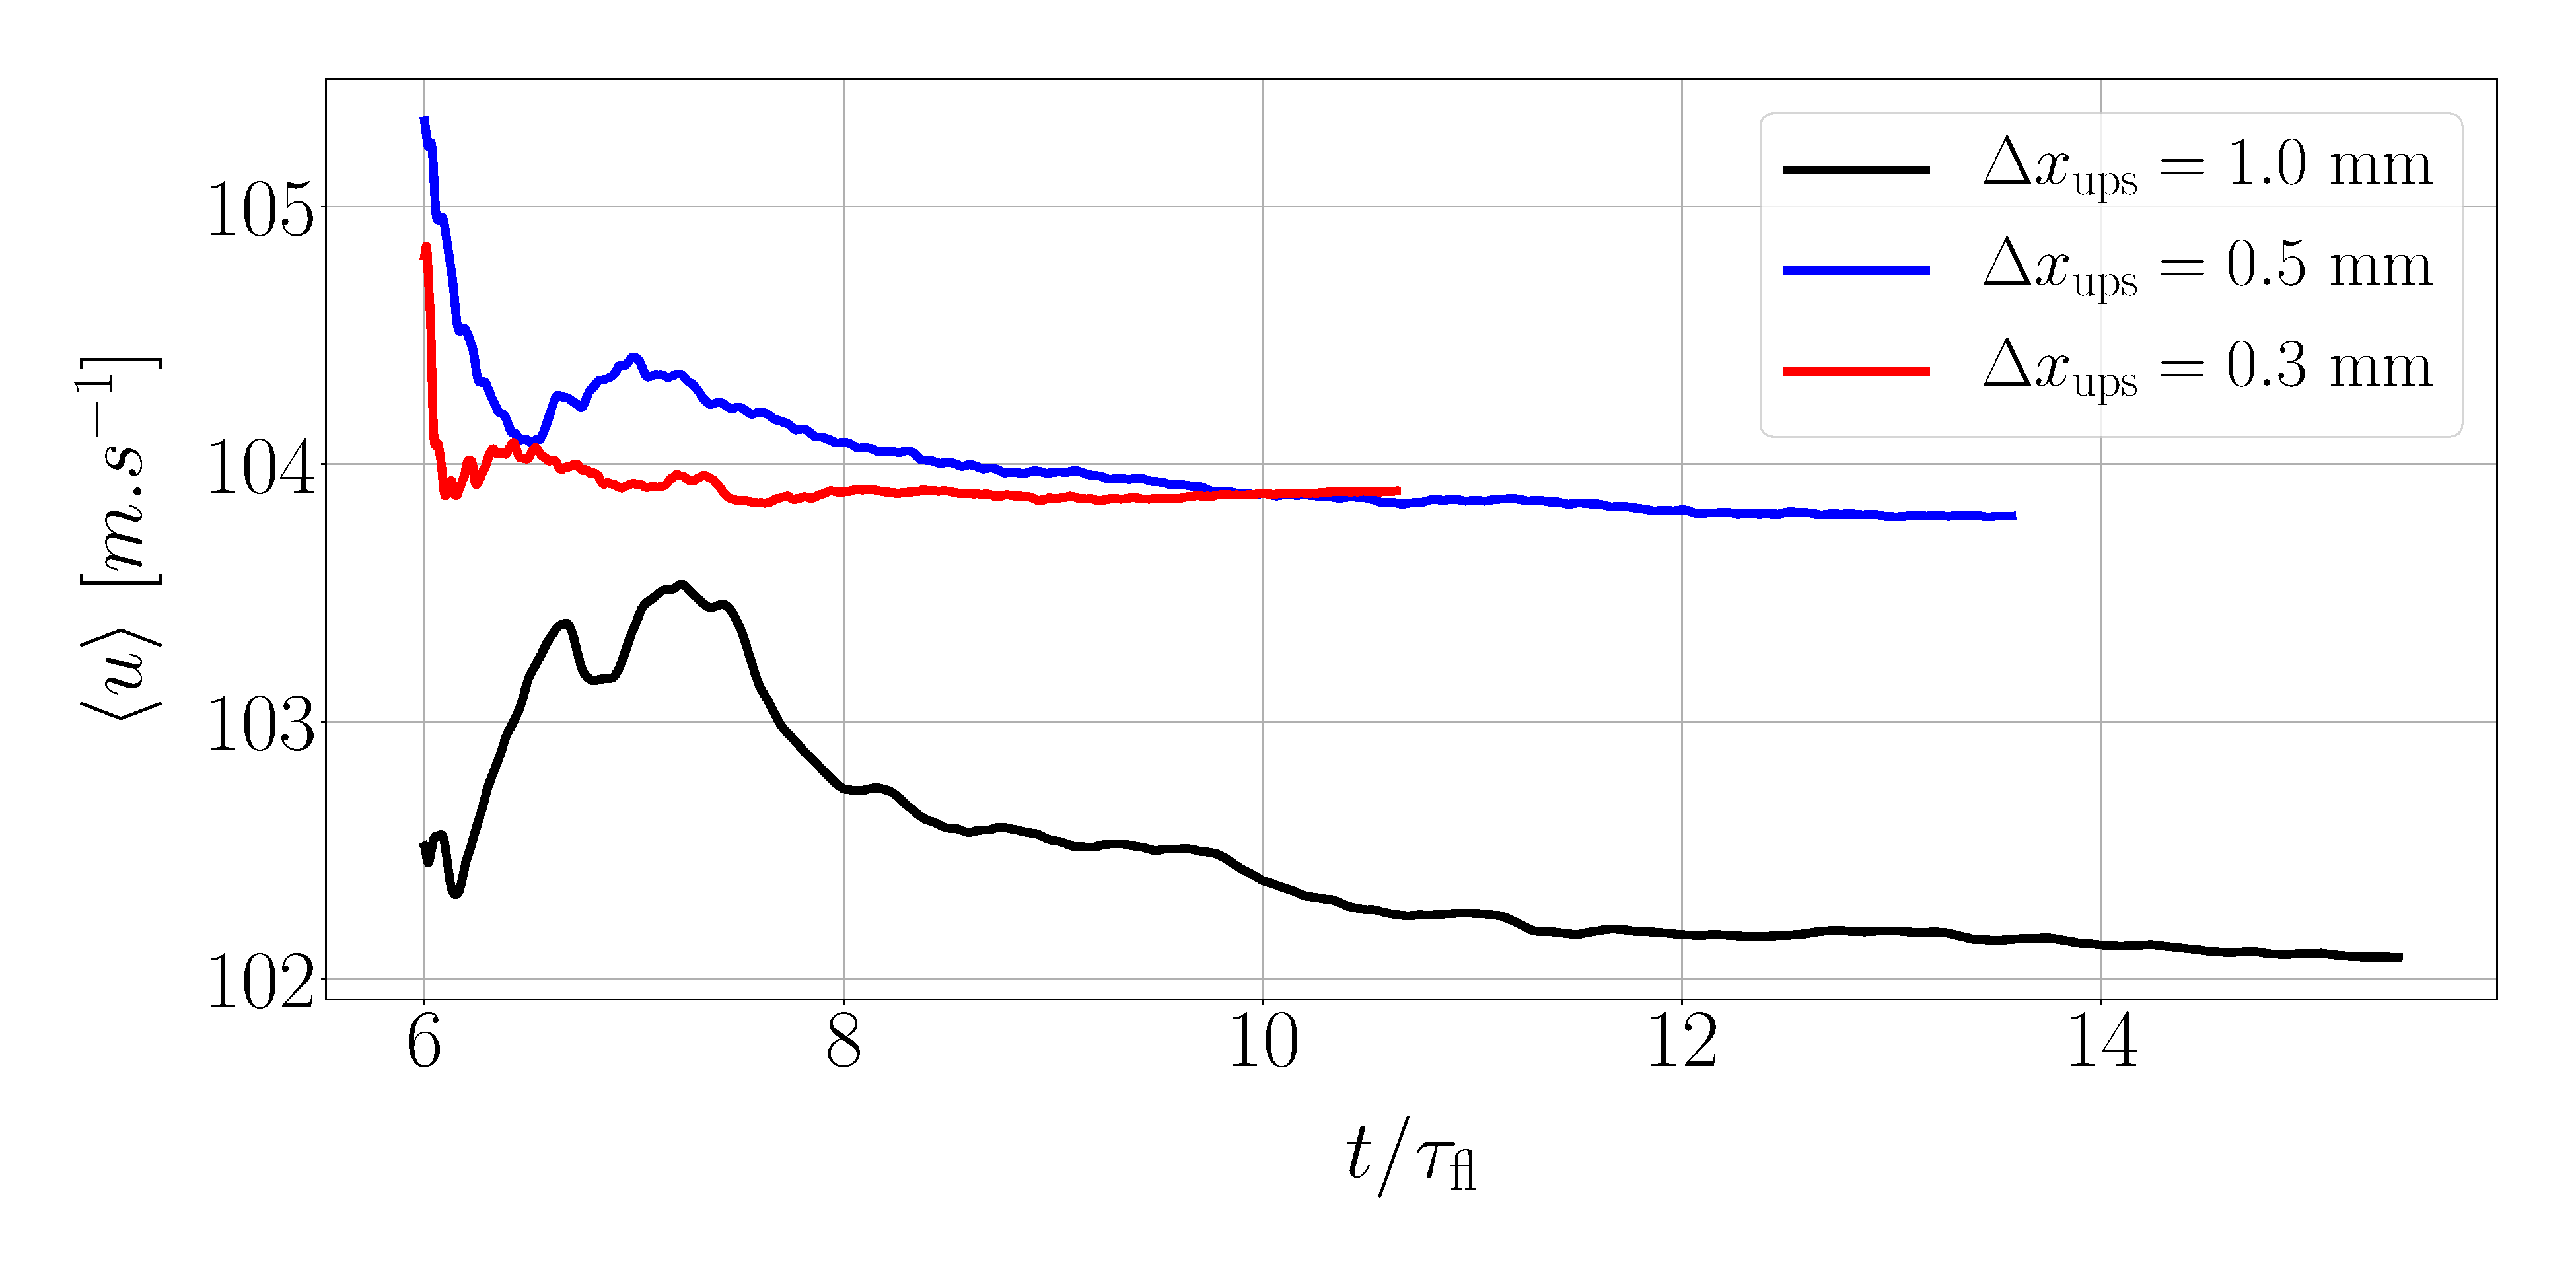
\includegraphics[scale=0.125]{./part2_developments/figures_ch5_resolved_JICF/results_ics_mesh_convergence_line_averages/U_MEAN.pdf}
   \caption{Mean axial velocity}
   %\label{} 
\end{subfigure}
\hfill
\begin{subfigure}[b]{0.45\textwidth}
	\centering
   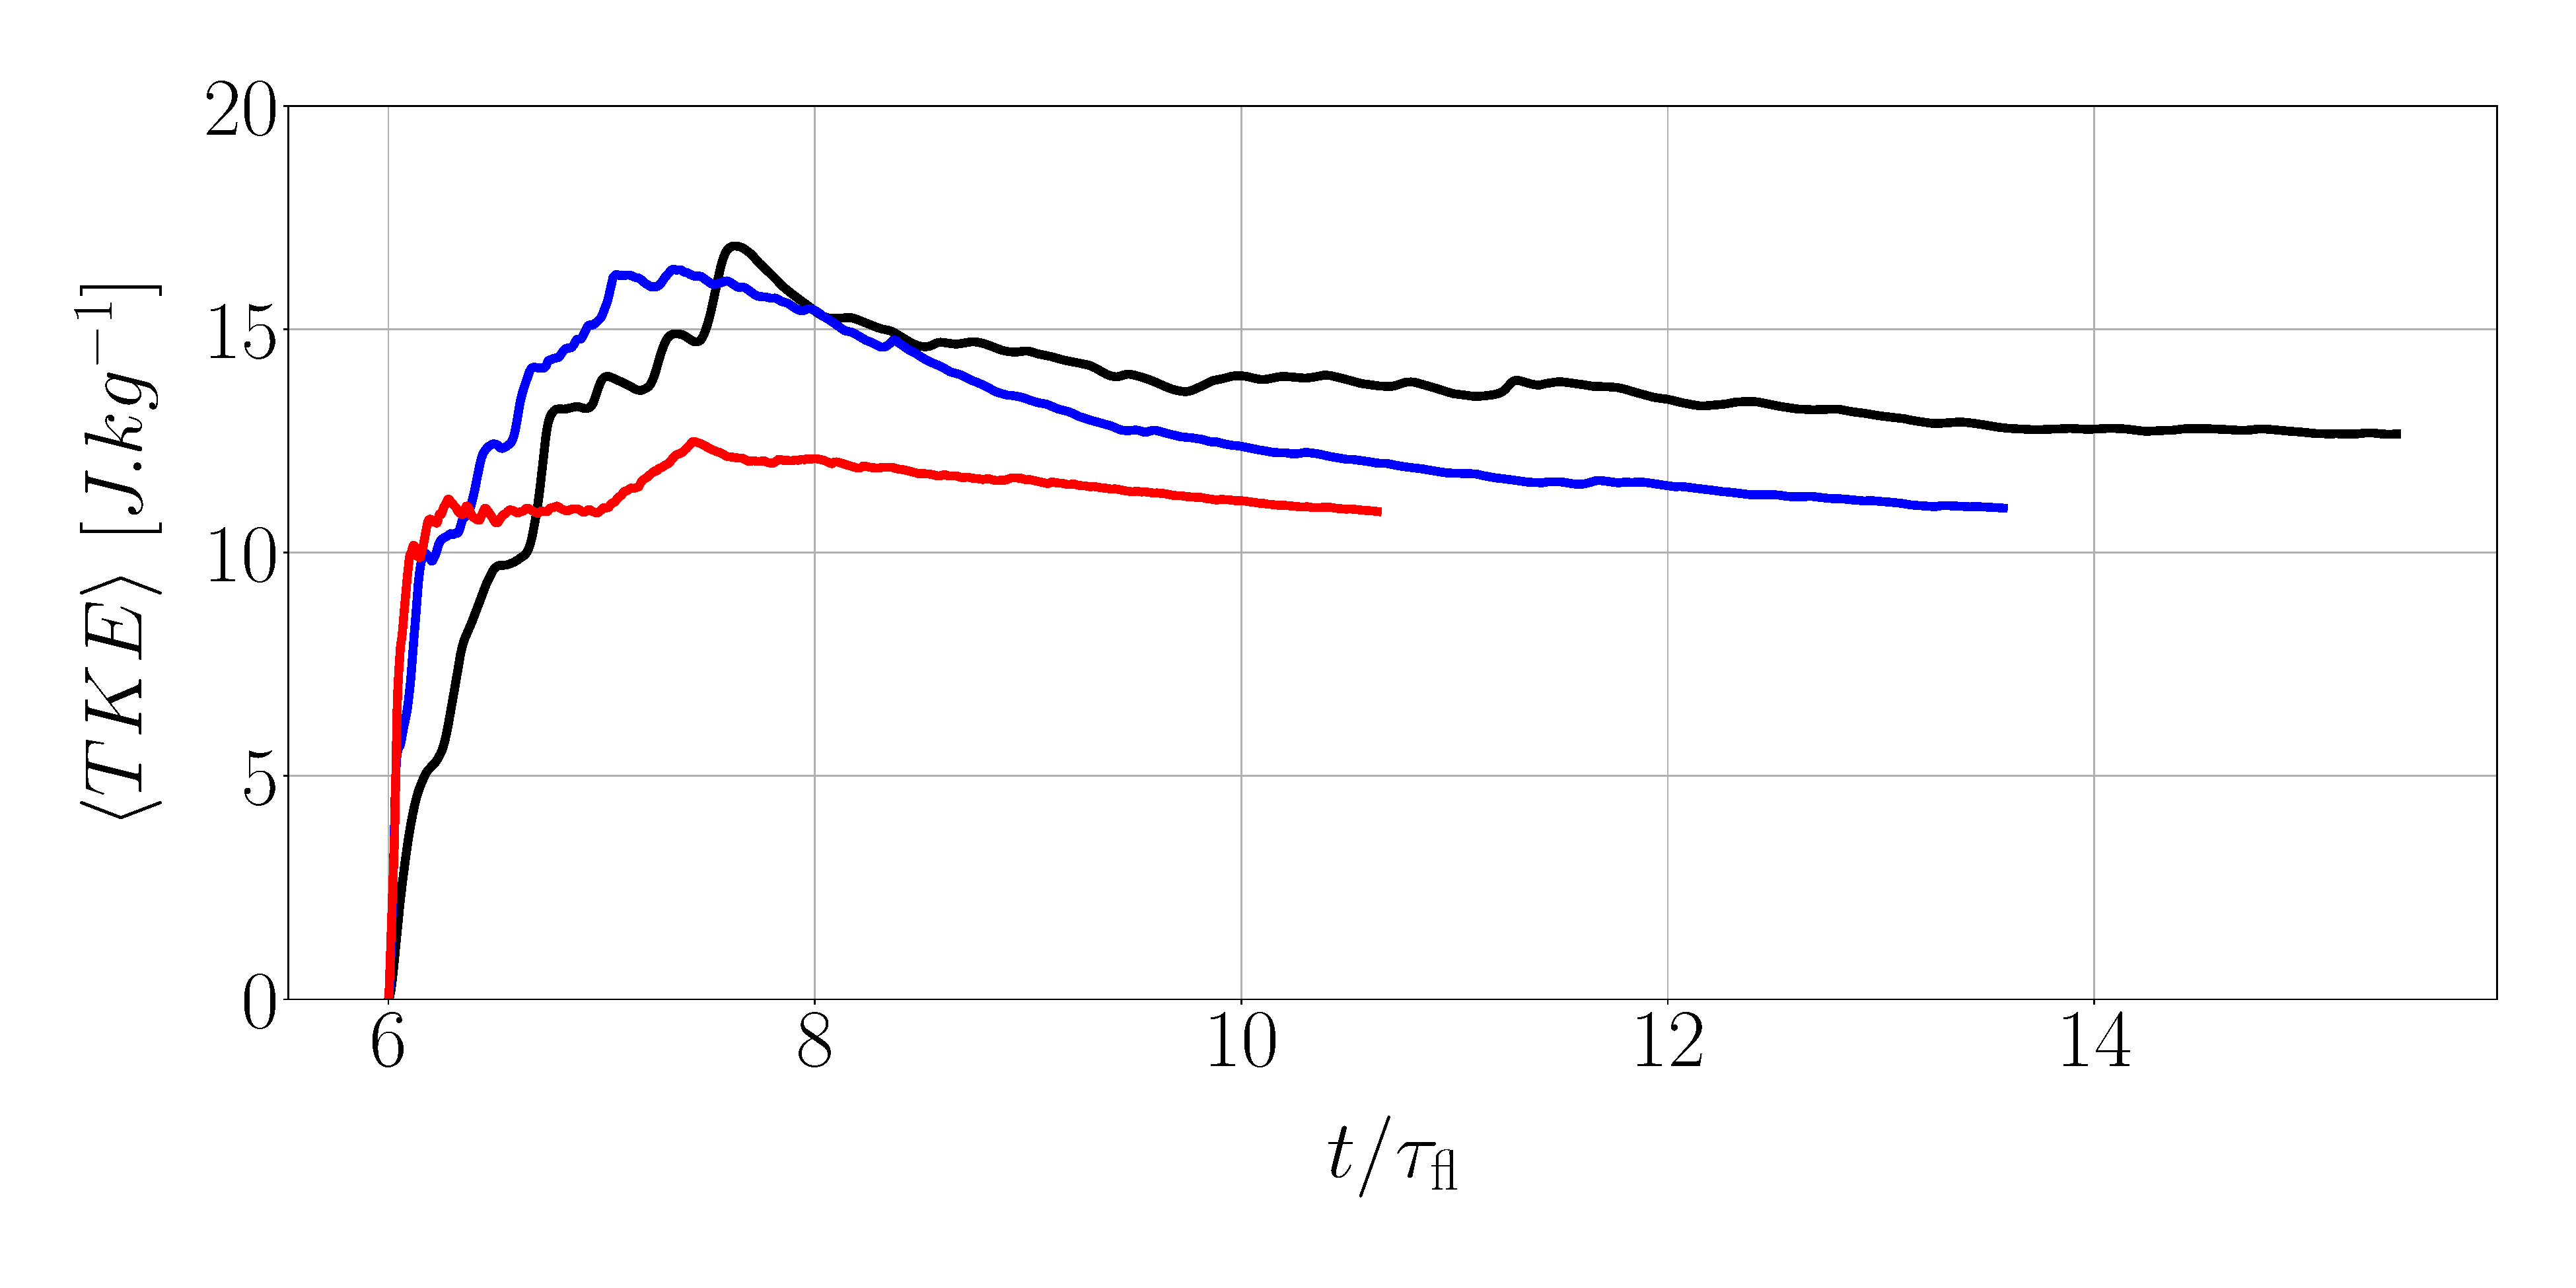
\includegraphics[scale=0.125]{./part2_developments/figures_ch5_resolved_JICF/results_ics_mesh_convergence_line_averages/TKE.pdf}
   \caption{Turbulent Kinetic Energy}
   %\label{}
\end{subfigure}
\caption{Convergence of line-integrated mean axial velocity and TKE with mesh resolution}
\label{fig:mesh_convergence_line_averages}
\end{figure}



Instantaneous snapshots of the fluctuating axial component $u'$ in the middle plane are shown in Figure \ref{fig:ics_mesh_independency_study_up_fields}. The black contours denote the lines with $u' = 0$. As shown, adding turbulence at the inlet introduces fluctuations that are transported downstream the domain. When no turbulence is added, fluctuations are not present (the black contours at the inlet are due to small numerical fluctuations of $u'$) except close to the walls, since they are created inside the boundary layer where flow is intrinsically turbulent. It is also observed that the characteristic length of the eddies changes when refining the mesh: for the coarsest mesh ($\Delta x_\mathrm{ups} = 1$ mm), these structures are generally large, while refining the mesh to $\Delta x_\mathrm{ups} = 0.5$ and $0.3$ mm reduced their size. 

%% OJO: Pope criterion
%
%To assess the quality of the meshes, it is useful to introduce a criterion for measuring the turbulent resolution. For such purpose, the Pope's criterion $M$ is employed \textbf{ref-pope-criterion}, which is calculated from the ratio between the resolved and sub-grid Turbulent Kinetic Energies,  $\mathrm{TKE}$ and $k_\mathrm{sgs}$ respectively:
%
%\begin{equation}
%M \left( \textbf{x}, t \right) = \frac{k_\mathrm{sgs} \left( \textbf{x}, t \right)}{k_\mathrm{sgs}  \left( \textbf{x}, t \right) + TKE \left( \textbf{x}, t \right)}
%\end{equation}
%
%$M$ represents therefore the ratio between the sub-grid (unresolved) and total TKEs in the domain, and depends on time and space. From its definition it follows that $M = 0$ corresponds to full resolution (i.e. DNS) and $M = 1$ to full modelling (i.e. RANS) of the turbulent flow field. The sub-grid TKE can be obtained from the following expression:
%
%
%\begin{equation}
%k_\mathrm{sgs} = \left( \frac{\nu_t}{0.18 \Delta x} \right)^2
%\end{equation}
%
%where $\nu_t$ is the turbulent kinematic viscosity as given by the dynamic Smagorinsky model \citepColor[germano_dynamic_1991]. 
%
%Figure \ref{fig:ics_mesh_independency_study_POPE_M_fields} shows instantenous fields of Pope's criterion for the four simulations performed. As observed, by reducing the element size more regions with values of $M$ closer to $0$ are present. For $\Delta x = 1$ mm there several zones where $M$ has high values. These ones are overall reduced when reducing the cell size to $0.5$ mm and further to $0.3$ mm. Between these last two cell sizes there are also differences in the $M$ field specially far from the walls. For all cases, the $M$ values close to the walls are higher than in the far-field, indicating that a finer resolution would be needed in the walls to properly capture the turbulent features of the boundary layer. Nevertheless, these ones remain around $M \approx 0.5$ for the meshes with $\Delta x = 0.5$ and $0.3$ mm, indicating enough resolution for LES simulations. Regarding the case without turbulence injection for $\Delta x = 0.5$ mm, the $M$ field shows higher values with respect to the case where turbulence is added, specially closer to the inlet and in the regions outside the boundary layer. 

In order to compare quantitatively the difference between meshes, the signals of $u'$ have been monitored with time at the probes shown by the white crosses in the top of Figure \ref{fig:ics_mesh_independency_study_up_fields}. Two probes have been located: one at 50 mm upstream the liquid inlet (x = 70 mm, probe A) and another one 1 mm upstream the liquid injection nozzle (x = 119 mm, probe B), both at a height of 8 mm from the bottom wall. The capability of the meshes to transport the resolved turbulent scales, which is of the order of the turbulent fluctuations displayed in Table \ref{tab:jicf_operating_conditions_turbulent_injection_parameters}, is then verified by comparing the fluctuations and spectra obtained with Fast Fourier Transform (FFT) at both probes in Figure \ref{fig:ics_mesh_independency_study_probes}. Time has been normalised with the flow-through time $\tau_\mathrm{fl}$, and the signals are shown for one passage of $\tau_\mathrm{fl}$ for easiness of visualization. For the coarsest mesh $\Delta x_\mathrm{ups} = 1$ mm (Figure \ref{fig:ics_mesh_independency_study_probes_dx1p0}), the $u'$ signal sampled closer to the nozzle (Probe B) shows similar magnitudes and frequencies to the signal sampled upstream (Probe A). Despite the characteristic peaks at frequencies of 8, 17 and 25 $\mathrm{kHz}$ with decreasing intensity for both probes, low frequencies below 10 $\mathrm{kHz}$ are excited. The spectrum at Probe B shows a higher relative intensity at these low frequencies with at 3 $\mathrm{kHz}$ not observed at probe A. This indicates that for this resolution, turbulent energy is not properly transported to the liquid injector. Furthermore, characteristic frequencies larger than 25 $\mathrm{kHz}$ cannot be capture, which is not the case for the rest of resolutions. When the mesh is refined to $\Delta x_\mathrm{ups} = 0.5$ mm (Figure \ref{fig:ics_mesh_independency_study_probes_dx0p5}), the small dominant frequencies are no longer relevant and the dominant frequencies are properly captured, as the match in the peaks of the spectra indicate. In this case, the frequencies 8 and 25 $\mathrm{kHz}$ have larger intensity than 17 $\mathrm{kHz}$. Refining the mesh to $\Delta x_\mathrm{ups} = 0.3$ mm (Figure \ref{fig:ics_mesh_independency_study_probes_dx0p3}) has no longer effect neither in the magnitude of the fluctuations nor in the spectrum. 

The fluctuations and FFT of the simulation performed without turbulence injection for the resolution $\Delta x_\mathrm{ups} = 0.5$ mm are shown Figure \ref{fig:ics_mesh_independency_study_probes_dx0p5_no_turb}. As expected, the magnitude of the fluctuations is lower than in the cases with synthetic turbulence. The spectrum shows that the energy content at low frequencies is high and that no clear dominant frequencies are found. \\

A final check on the mesh capability to transport turbulent can be done by calculating the Turbulent Kinetic Energy (TKE) at the probes A and B for simulation where turbulence is transported. TKE can be defined by the following formula:

\begin{equation}
TKE = \frac{1}{2} \left( \overline{u'^2} + \overline{v'^2} + \overline{w'^2} \right)
\end{equation}

Note that, unlike in Eq. (\ref{eq:line_averaged_u_and_TKE}), the TKE is not averaged along a line but represents the resolved energy contained in the eddies at probes A and B. 
Results are shown in Figure \ref{fig:TKE_vs_dx_in_probes}. As observed ... \\

Finally, the profiles of mean axial velocity $\overline{u}$ and TKE are plotting along the vertical line shown in Figure \ref{fig:ics_mesh_independency_study_up_fields} right for the half-width of the channel. The results are shown in Figure \ref{fig:ics_mesh_independency_study_mean_profiles}. The mean velocity profile is properly captured for all meshes, despite slight variations within the boundary layer where the mean velocity evolves from 0 to the velocity in the outer layer, which is constant and equal in all cases (despite some fluctuations due to numerical noise). The boundary layer thickness (observed in the evolution of both $\overline{u}$ and $TKE$) is around 5 mm, which is consistent with the experimental values reported in \citeColor[becker_breakup_2002]. Part of the liquid jet is comprised within the boundary layer, as it is illustrated in Figure \ref{fig:Umean_profile_with_jet} where the velocity profile is displayed with a snapshot of one of the liquid simulations discussed later in this report. The $TKE$ profiles for the turbulent cases show that the turbulent energy in the outer layer (z > 5 $mm$) is similar for the resolutions $\Delta x_\mathrm{ups} = 0.5$ and $0.3$ mm, but lower for the thicker resolution of 1 mm. For $\Delta x_\mathrm{ups} = 0.5$ mm, the profile with turbulence shows larger values of TKE than the case without turbulence injected, as expected. Within the boundary layer, however, convergence in terms of resolution is never achieved, since the profile always changes when the mesh is refined in the inner layer (up to z = 2 mm). The smallest scales of for this region are assumed to be of the order of \textbf{XX??} (see Appendix \textbf{XX??}), which cannot be captured not even with the finest cell size of $\Delta x_\mathrm{ups} = 0.3$ mm. A proper resolution at this region would require cell sizes corresponding to DNS, which is unfeasible for the case studied. Nevertheless, the values of TKE for z > 2 mm, including the energy decrease from this point up to the freestream, is converged for the resolution $\Delta x_\mathrm{ups} = 0.5$ mm. \\

From these results, the simulation with the mesh resolution $\Delta x_\mathrm{ups} = 0.5$ mm was chosen as initial solution for performing the two-phase simulations. As shown, this mesh size allows for a proper turbulent transport (frequencies and energy content) with a moderable cost: Table \ref{tab:jicf_mesh_independence_gaseous_study} shows that decreasing the resolution from 1 to 0.5 mm supposed an increase of 5 million of elements, while further refining from 0.5 to 0.3 mm adds up to 28 million. The turbulent content in the inner part of the turbulent layer is not properly resolved, which could have an effect on the jet atomization and has not been check in this work (\textbf{XX Maybe NOT ?? CHECK atomization characteristics and SLI in turbulence vs no-turbulence simulations XX}). It, however, does not have an effect on the trajectory, as it is shown in $\S$\ref{subsec:ch5_jet_trajectories_results}. A local refinement on the boundary layer (inflation layer) could help to converge the TKE profiles without a large increase in the cost of the simulations.



\begin{figure}[ht]
\centering
\includeinkscape[inkscapelatex=false,scale=0.75]{./part2_developments/figures_ch5_resolved_JICF/results_ics_mesh_convergence_mesh_and_up/up_field_instantaneous_both}
\caption[Instantaneous $u'$ fields from gaseous simulation for the high Weber case]{Instantaneous $u'$ fields from gaseous simulation for the high Weber case. The right column shows a zoomed-in view of the dashed rectangle from the left column. The black contours indicate the lines with zero instantaneous fluctuation $u' = 0$. From top to bottom $\Delta x_\mathrm{ups} = 1, 0.5, 0.3$ mm.}
\label{fig:ics_mesh_independency_study_up_fields}
\end{figure}

%\begin{figure}[ht]
%\centering
%\includeinkscape[inkscapelatex=false,scale=0.75]{./part2_developments/figures_ch5_resolved_JICF/results_ics_mesh_convergence_POPE/pope_instantaneous_all}
%\caption[]{Views of Pope criterion}
%\label{fig:ics_mesh_independency_study_POPE_M_fields}
%\end{figure}

\clearpage

\begin{figure}[ht]
\centering
\begin{subfigure}[b]{1.0\textwidth}
	\centering   
	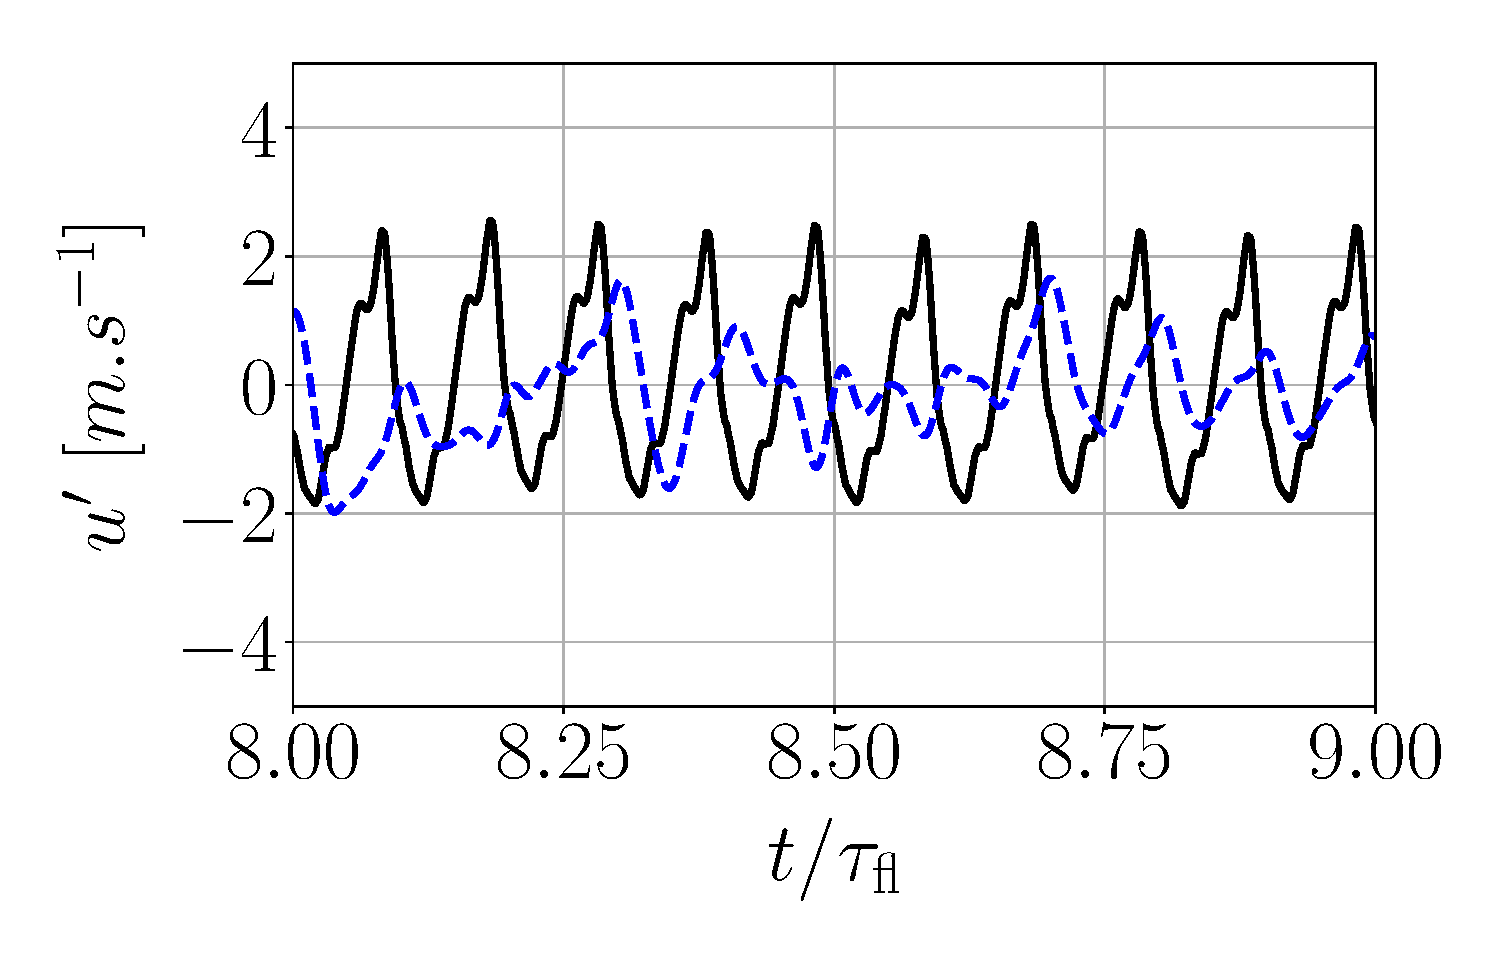
\includegraphics[scale=0.28]{./part2_developments/figures_ch5_resolved_JICF/results_ics_mesh_convergence_probes/up_dx1p0.pdf}
	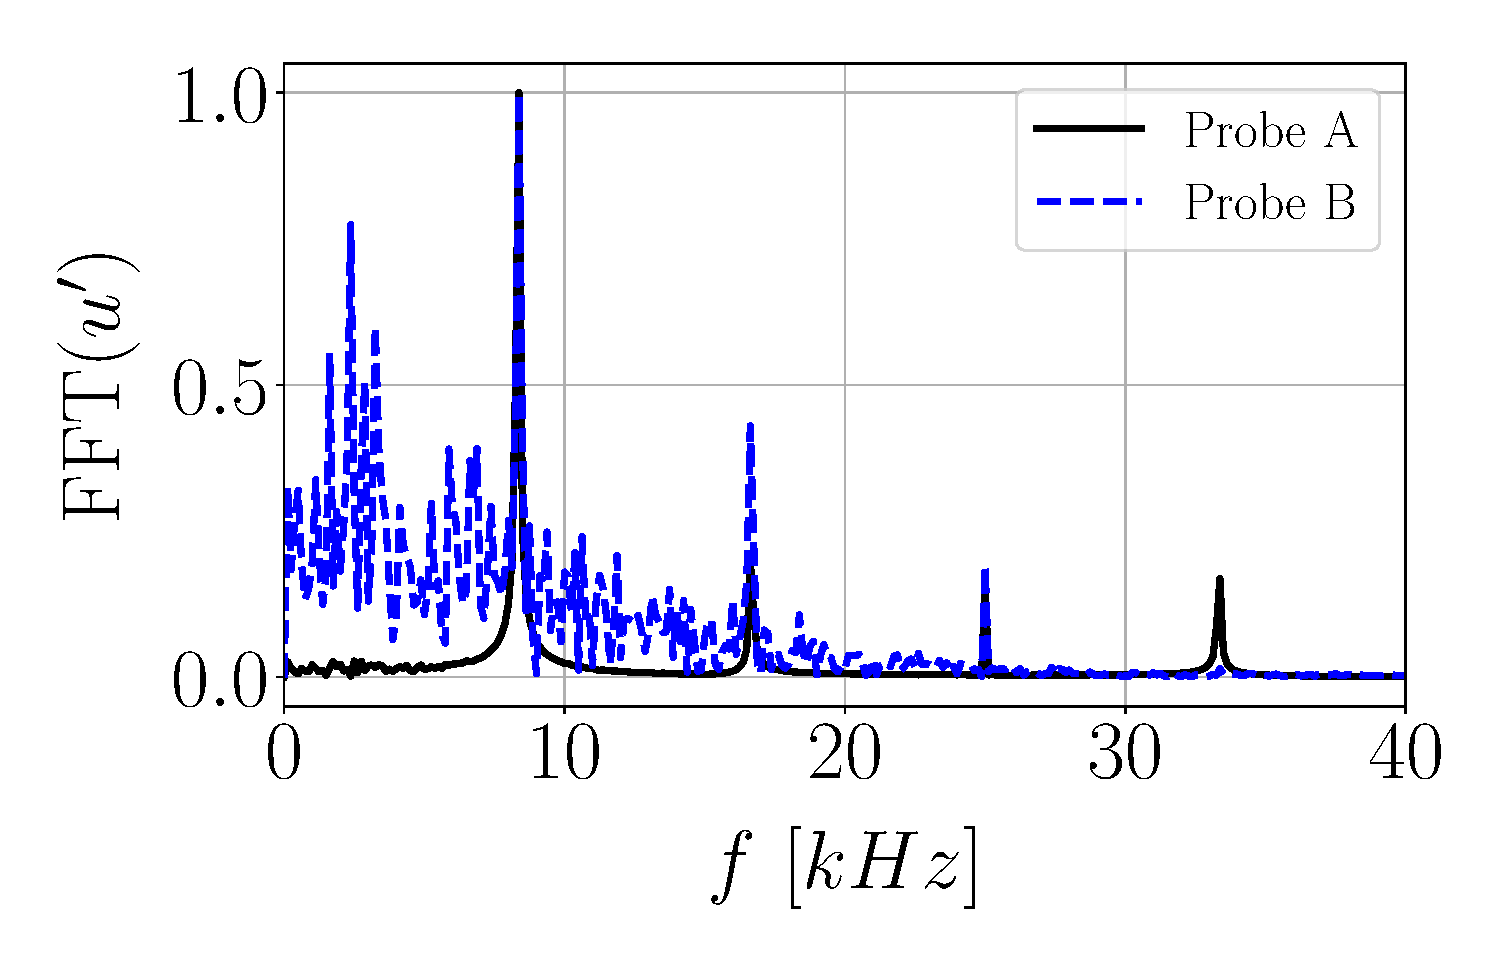
\includegraphics[scale=0.28]{./part2_developments/figures_ch5_resolved_JICF/results_ics_mesh_convergence_probes/spectra_linear_scale_dx1p0.pdf}
%	\subfloat[\centering]{{\includegraphics[scale=0.20]{./part2_developments/figures_ch5_resolved_JICF/results_ics_mesh_convergence_probes/up_dx1p0.eps} }}%
%    \qquad
%    \subfloat[\centering]{{ \includegraphics[scale=0.20]{./part2_developments/figures_ch5_resolved_JICF/results_ics_mesh_convergence_probes/spectra_linear_scale_dx1p0.eps} }}%
   \caption{Mesh $\Delta x_\mathrm{ups} = 1$ mm}
   \label{fig:ics_mesh_independency_study_probes_dx1p0}
\end{subfigure}


\vskip\baselineskip

\begin{subfigure}[b]{1.0\textwidth}
	\centering
   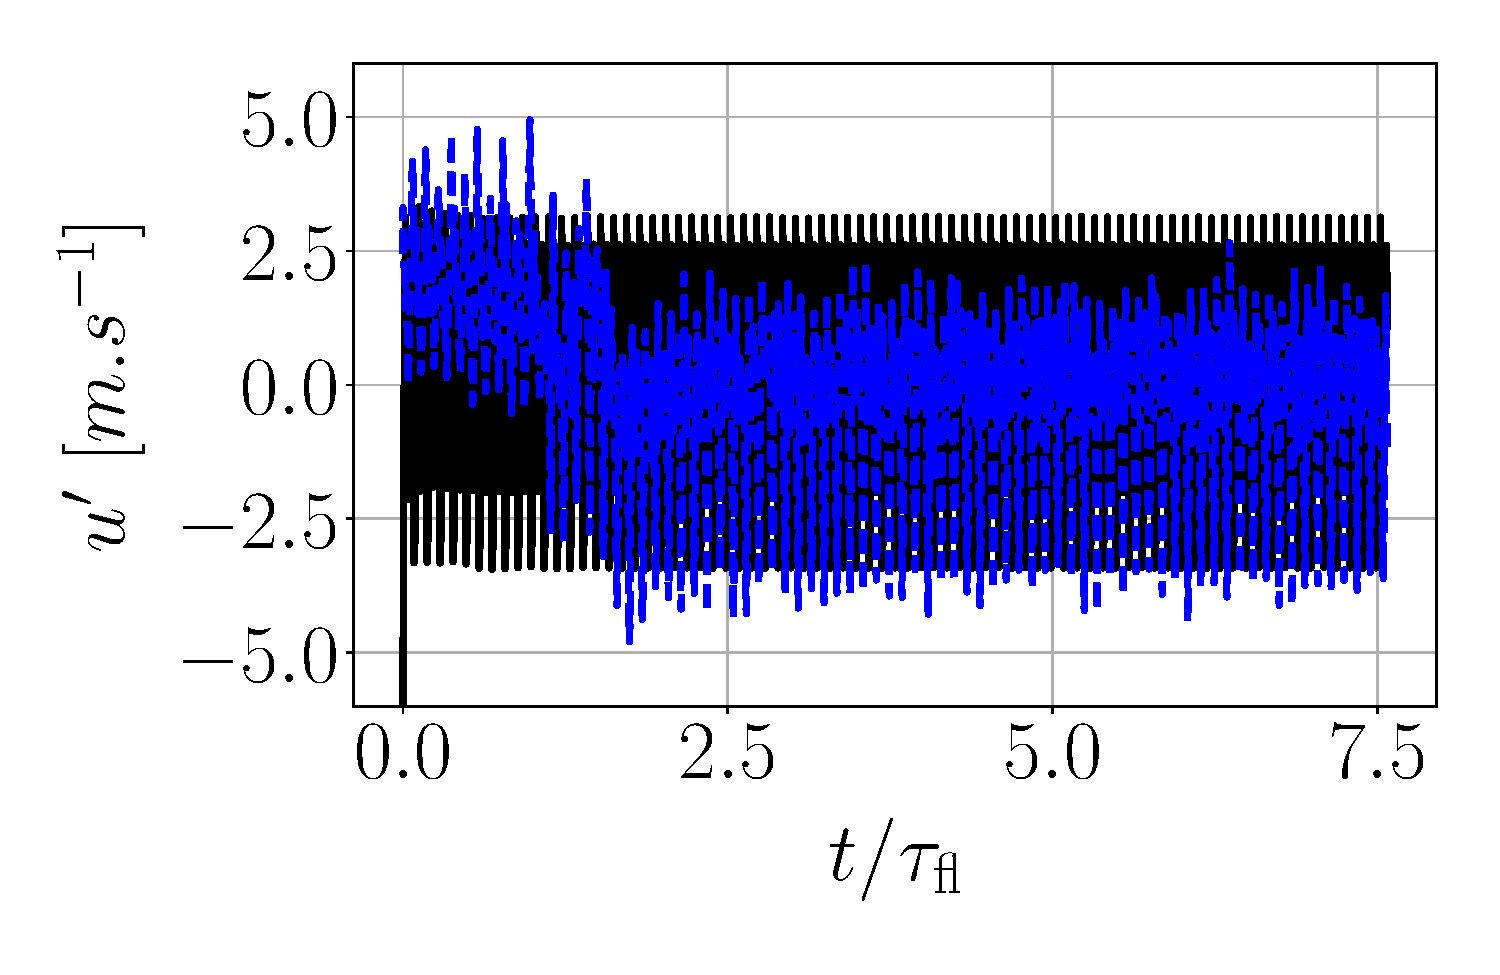
\includegraphics[scale=0.28]{./part2_developments/figures_ch5_resolved_JICF/results_ics_mesh_convergence_probes/up_dx0p5.pdf}
   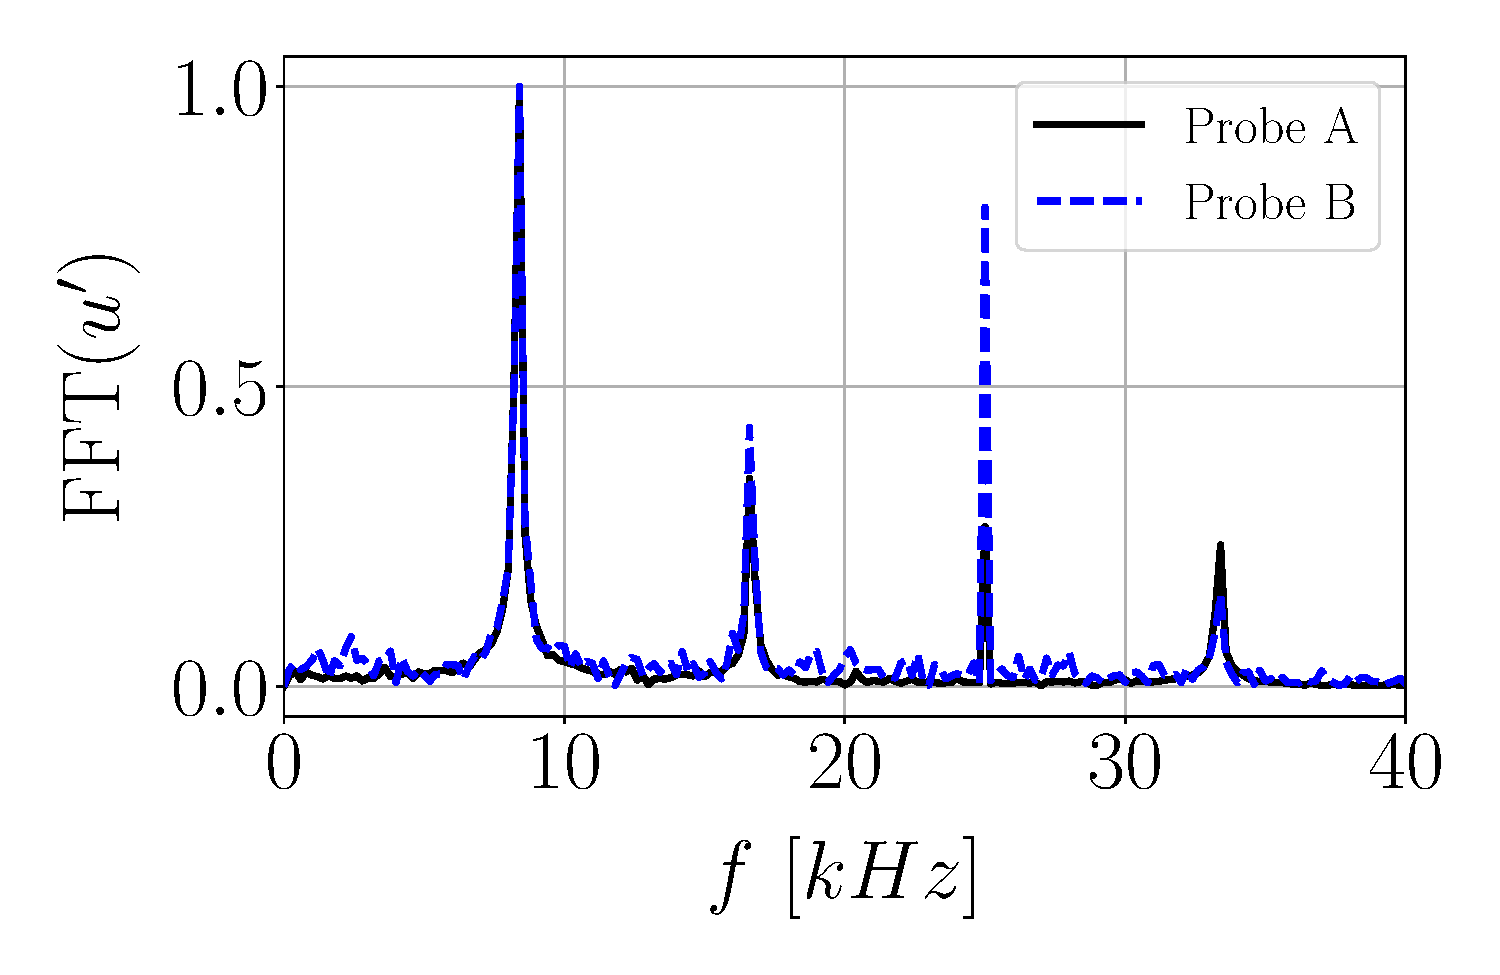
\includegraphics[scale=0.28]{./part2_developments/figures_ch5_resolved_JICF/results_ics_mesh_convergence_probes/spectra_linear_scale_dx0p5.pdf}
   \caption{Mesh $\Delta x_\mathrm{ups} = 0.5$ mm}
   \label{fig:ics_mesh_independency_study_probes_dx0p5}
\end{subfigure}

\vskip\baselineskip

\begin{subfigure}[b]{1.0\textwidth}
	\centering
   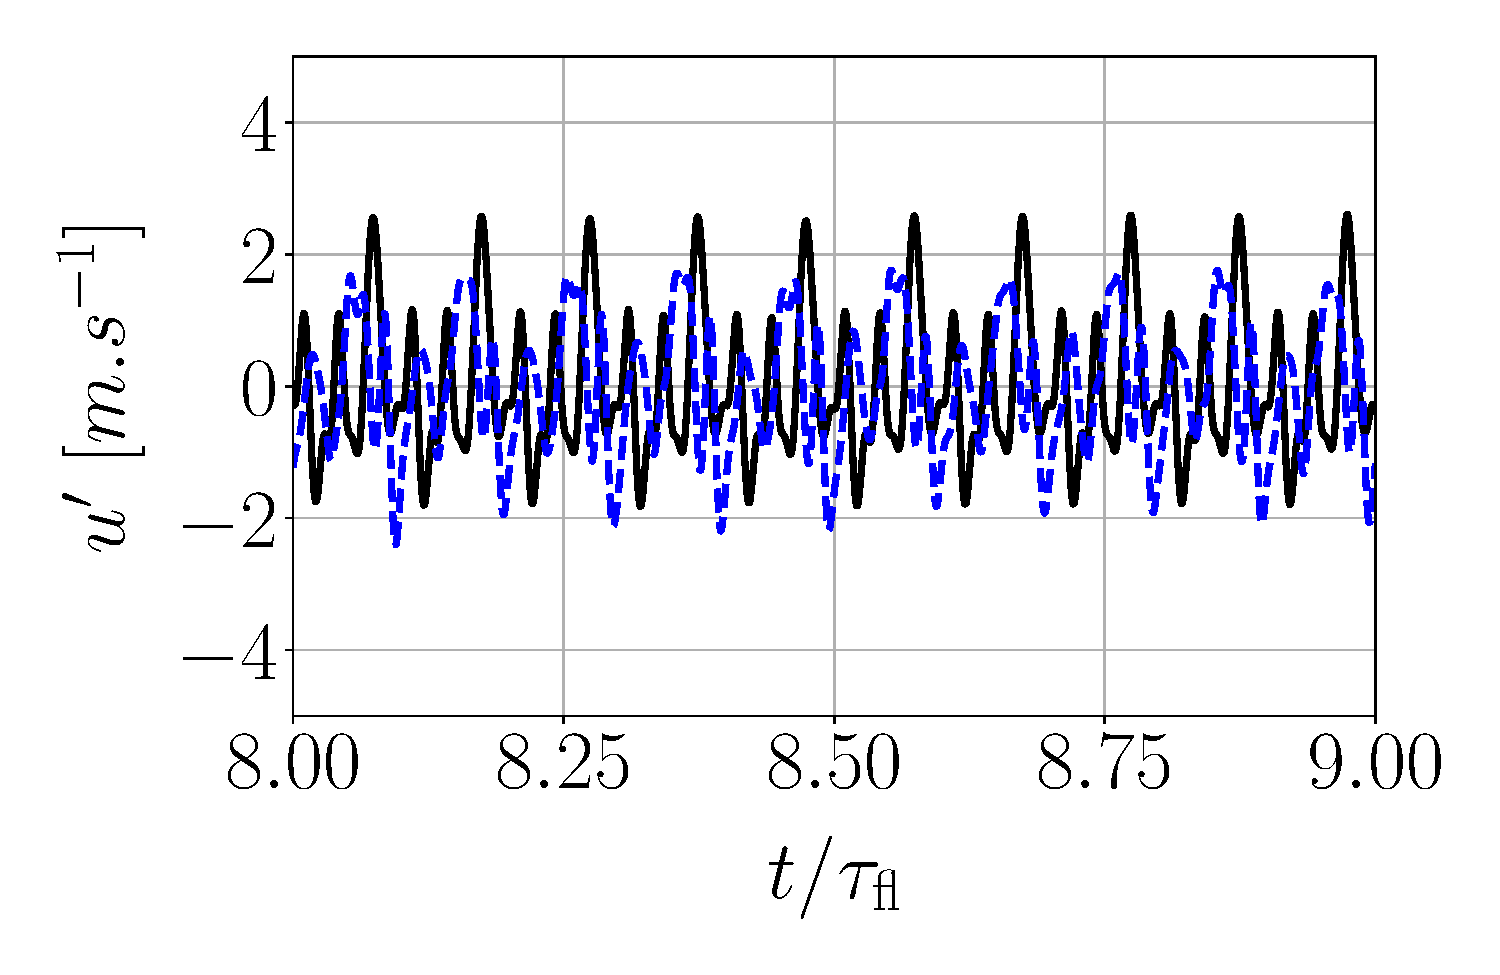
\includegraphics[scale=0.28]{./part2_developments/figures_ch5_resolved_JICF/results_ics_mesh_convergence_probes/up_dx0p3.pdf}
   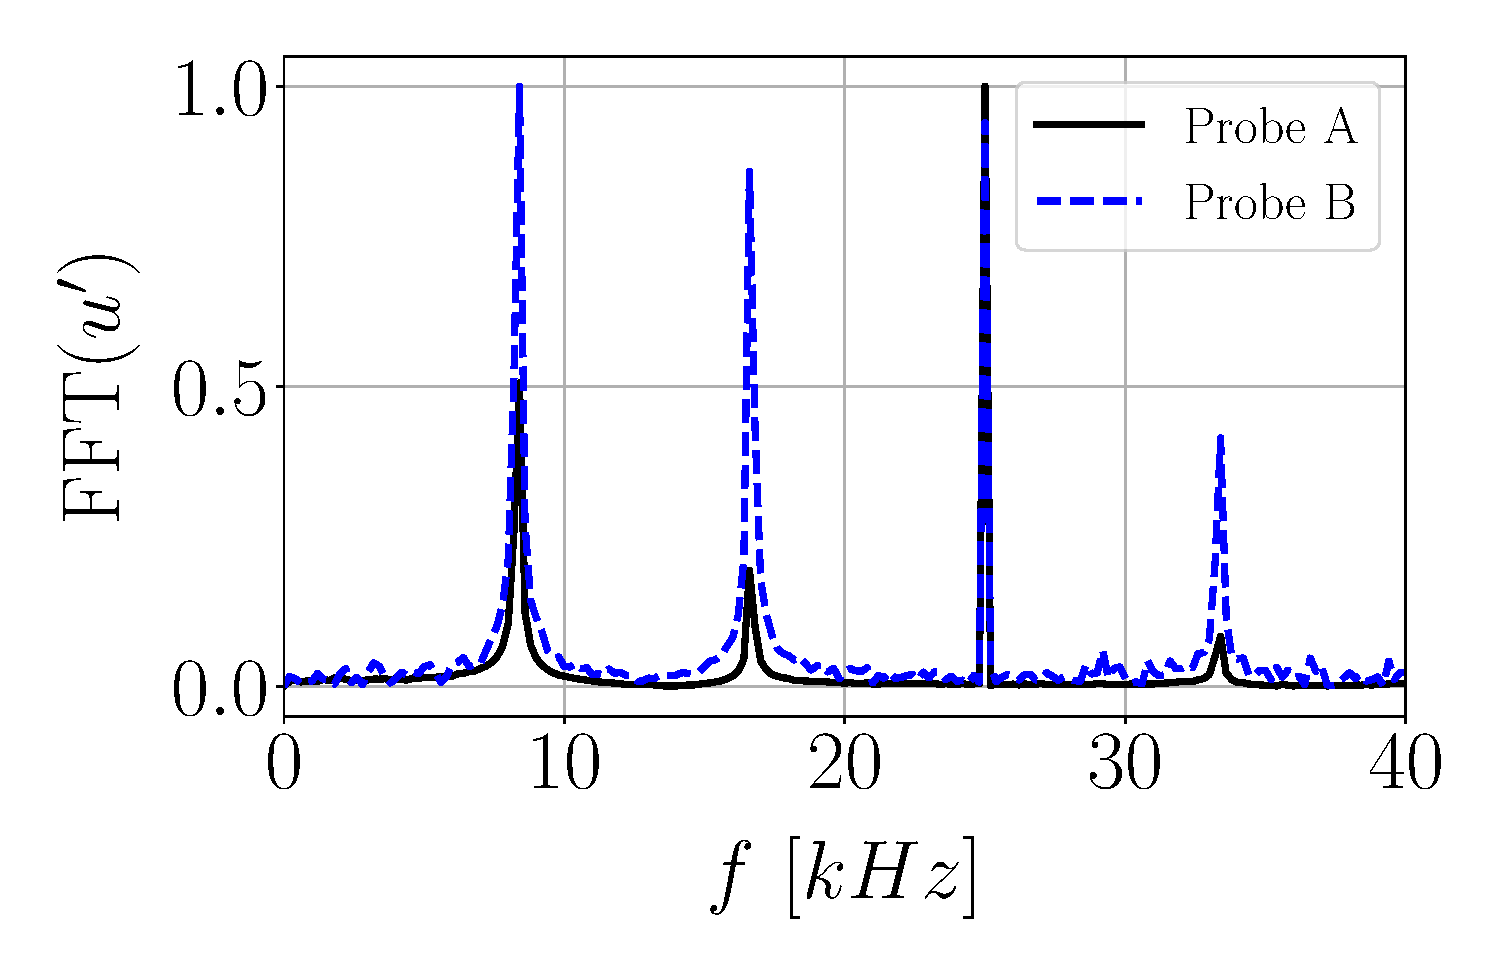
\includegraphics[scale=0.28]{./part2_developments/figures_ch5_resolved_JICF/results_ics_mesh_convergence_probes/spectra_linear_scale_dx0p3.pdf}
   \caption{{Mesh $\Delta x_\mathrm{ups} = 0.3$ mm}}
   \label{fig:ics_mesh_independency_study_probes_dx0p3}
\end{subfigure}


\vskip\baselineskip

\begin{subfigure}[b]{1.0\textwidth}
	\centering
   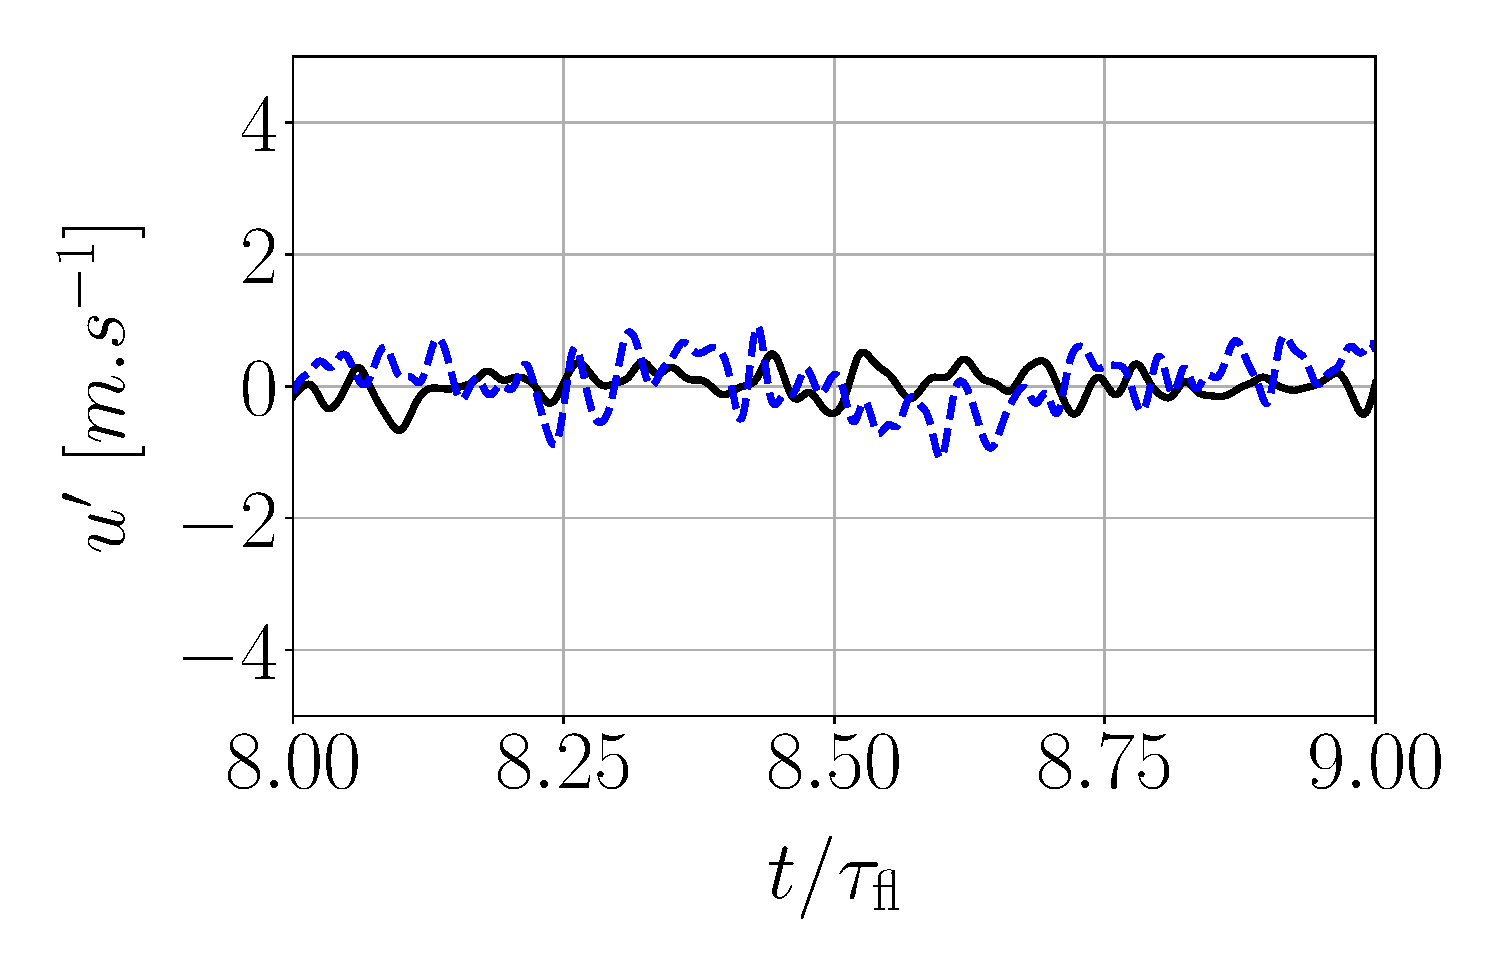
\includegraphics[scale=0.28]{./part2_developments/figures_ch5_resolved_JICF/results_ics_mesh_convergence_probes/up_dx0p5_no_turb.pdf}
   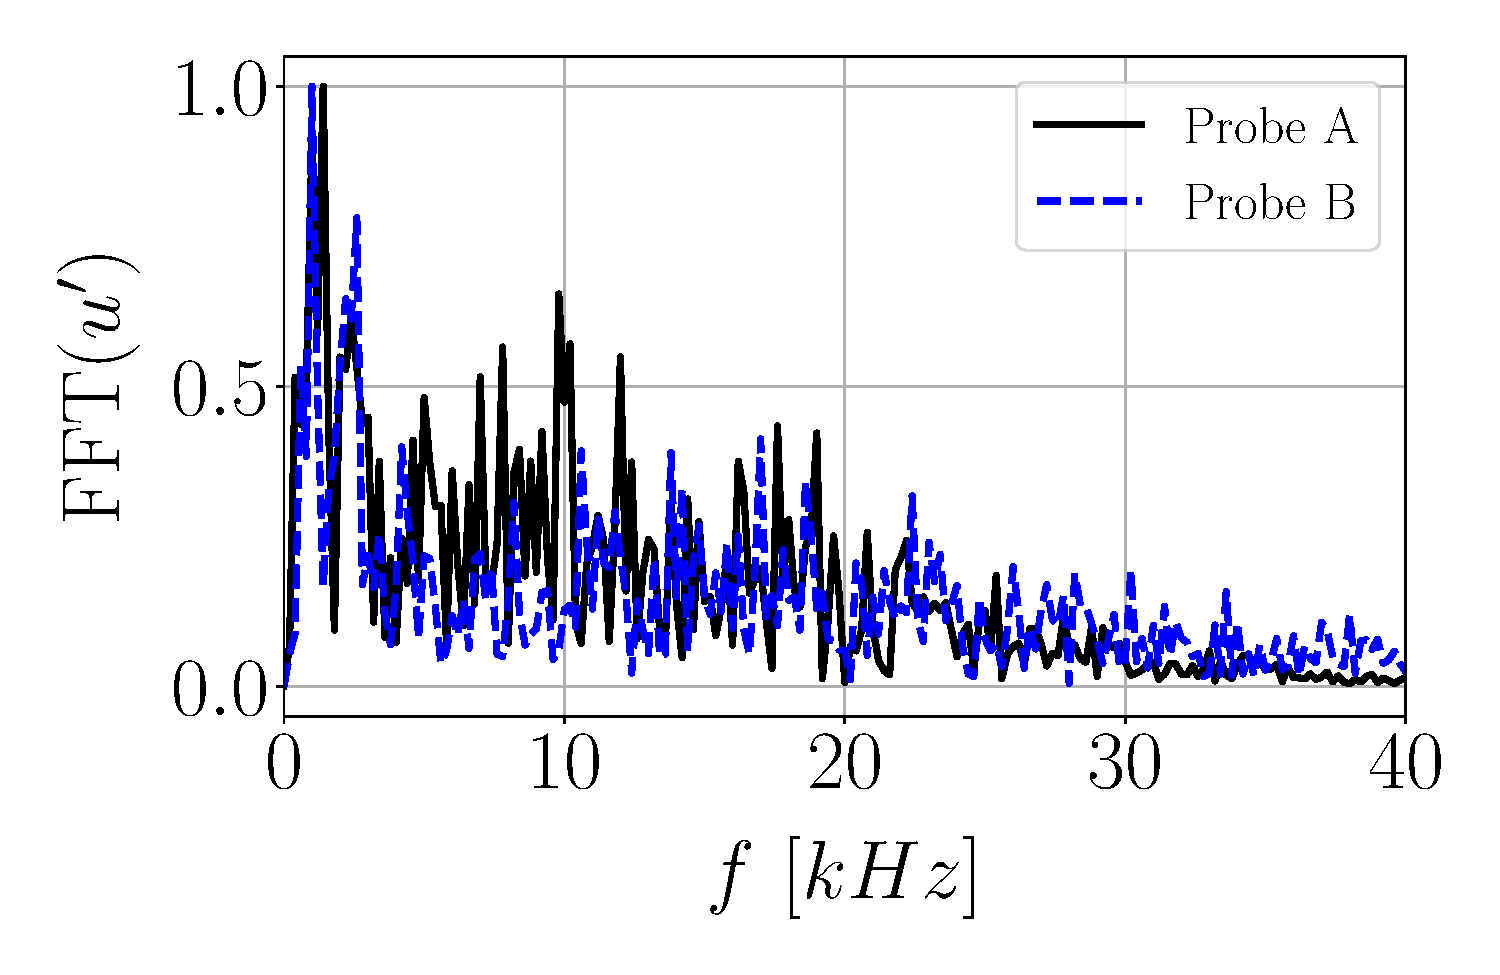
\includegraphics[scale=0.28]{./part2_developments/figures_ch5_resolved_JICF/results_ics_mesh_convergence_probes/spectra_linear_scale_dx0p5_no_turb.pdf}
   \caption{Mesh $\Delta x_\mathrm{ups} = 0.5$ mm without turbulence injection}
   \label{fig:ics_mesh_independency_study_probes_dx0p5_no_turb}
\end{subfigure}

\caption[Axial velocity fluctuations and associated frequencies at the sampling probes for the simulations at high Weber number.]{
Axial velocity fluctuations and associated frequencies at the sampling probes for the simulations at high Weber number. \textsl{Left}: $u'$ fluctuations. \textsl{Right}: spectra of the fluctuations obtained through FFT.}
\label{fig:ics_mesh_independency_study_probes}
\end{figure}




\clearpage


%\begin{figure}[ht]
%\centering
%\begin{subfigure}[b]{0.3\textwidth}
%	\centering
%   \includegraphics[scale=0.20]{./part2_developments/figures_ch5_resolved_JICF/results_ics_mesh_convergence_probes/up_dx1p0.eps}
%   %\caption{}
%   %\label{} 
%\end{subfigure}
%\hfill
%\begin{subfigure}[b]{0.3\textwidth}
%	\centering
%   \includegraphics[scale=0.20]{./part2_developments/figures_ch5_resolved_JICF/results_ics_mesh_convergence_probes/up_dx0p5.eps}
%   %\caption{}
%   %\label{} 
%\end{subfigure}
%\hfill
%\begin{subfigure}[b]{0.3\textwidth}
%	\centering
%   \includegraphics[scale=0.20]{./part2_developments/figures_ch5_resolved_JICF/results_ics_mesh_convergence_probes/up_dx0p3.eps}
%   %\caption{}
%   %\label{} 
%\end{subfigure}
%
%\vskip\baselineskip
%
%\begin{subfigure}[b]{0.3\textwidth}
%	\centering
%   \includegraphics[scale=0.20]{./part2_developments/figures_ch5_resolved_JICF/results_ics_mesh_convergence_probes/spectra_linear_scale_dx1p0.eps}
%   \caption{}
%   %\label{}
%\end{subfigure}
%\hfill
%\begin{subfigure}[b]{0.3\textwidth}
%	\centering
%   \includegraphics[scale=0.20]{./part2_developments/figures_ch5_resolved_JICF/results_ics_mesh_convergence_probes/spectra_linear_scale_dx0p5.eps}
%   \caption{}
%   %\label{}
%\end{subfigure}
%\hfill
%\begin{subfigure}[b]{0.3\textwidth}
%	\centering
%   \includegraphics[scale=0.20]{./part2_developments/figures_ch5_resolved_JICF/results_ics_mesh_convergence_probes/spectra_linear_scale_dx0p3.eps}
%   \caption{}
%   %\label{}
%\end{subfigure}
%
%\caption[YAP]{Probes}
%\label{fig:ics_mesh_independency_study_probes}
%\end{figure}






\begin{figure}[ht]
	\centering
	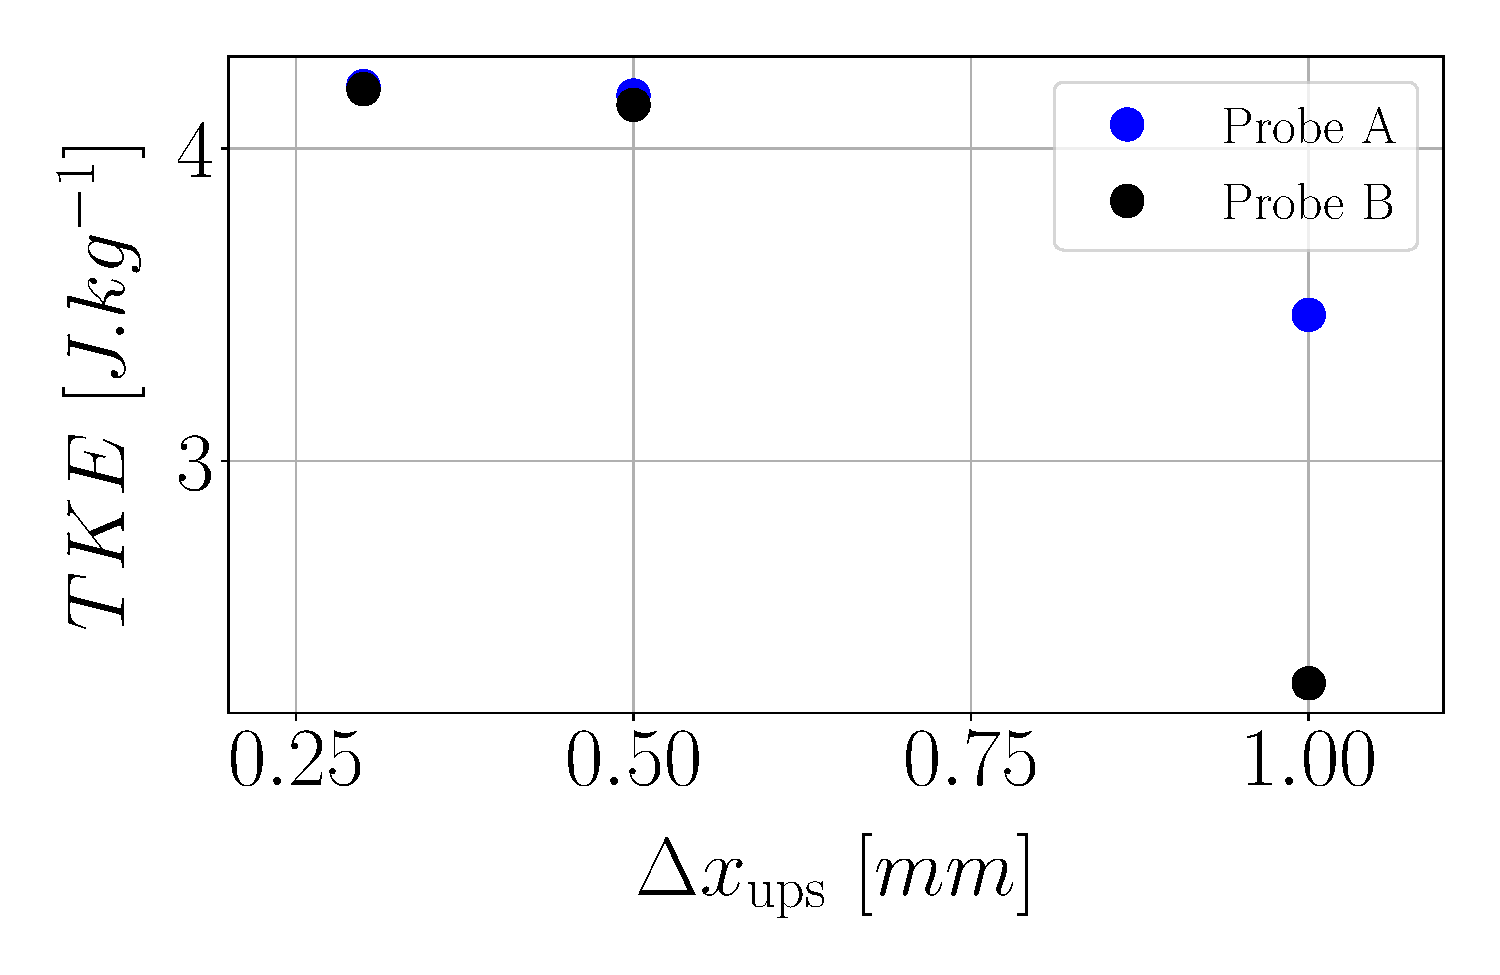
\includegraphics[scale=0.28]{./part2_developments/figures_ch5_resolved_JICF/results_ics_mesh_convergence_probes/TKE_vs_dx_in_probes.pdf}
   \caption{Variation in Turbulent Kinetic Energy in probes A and B with upstream mesh resolution.}
   \label{fig:TKE_vs_dx_in_probes}
\end{figure}


\begin{figure}[ht]
\centering
\begin{subfigure}[b]{0.45\textwidth}
	\centering
   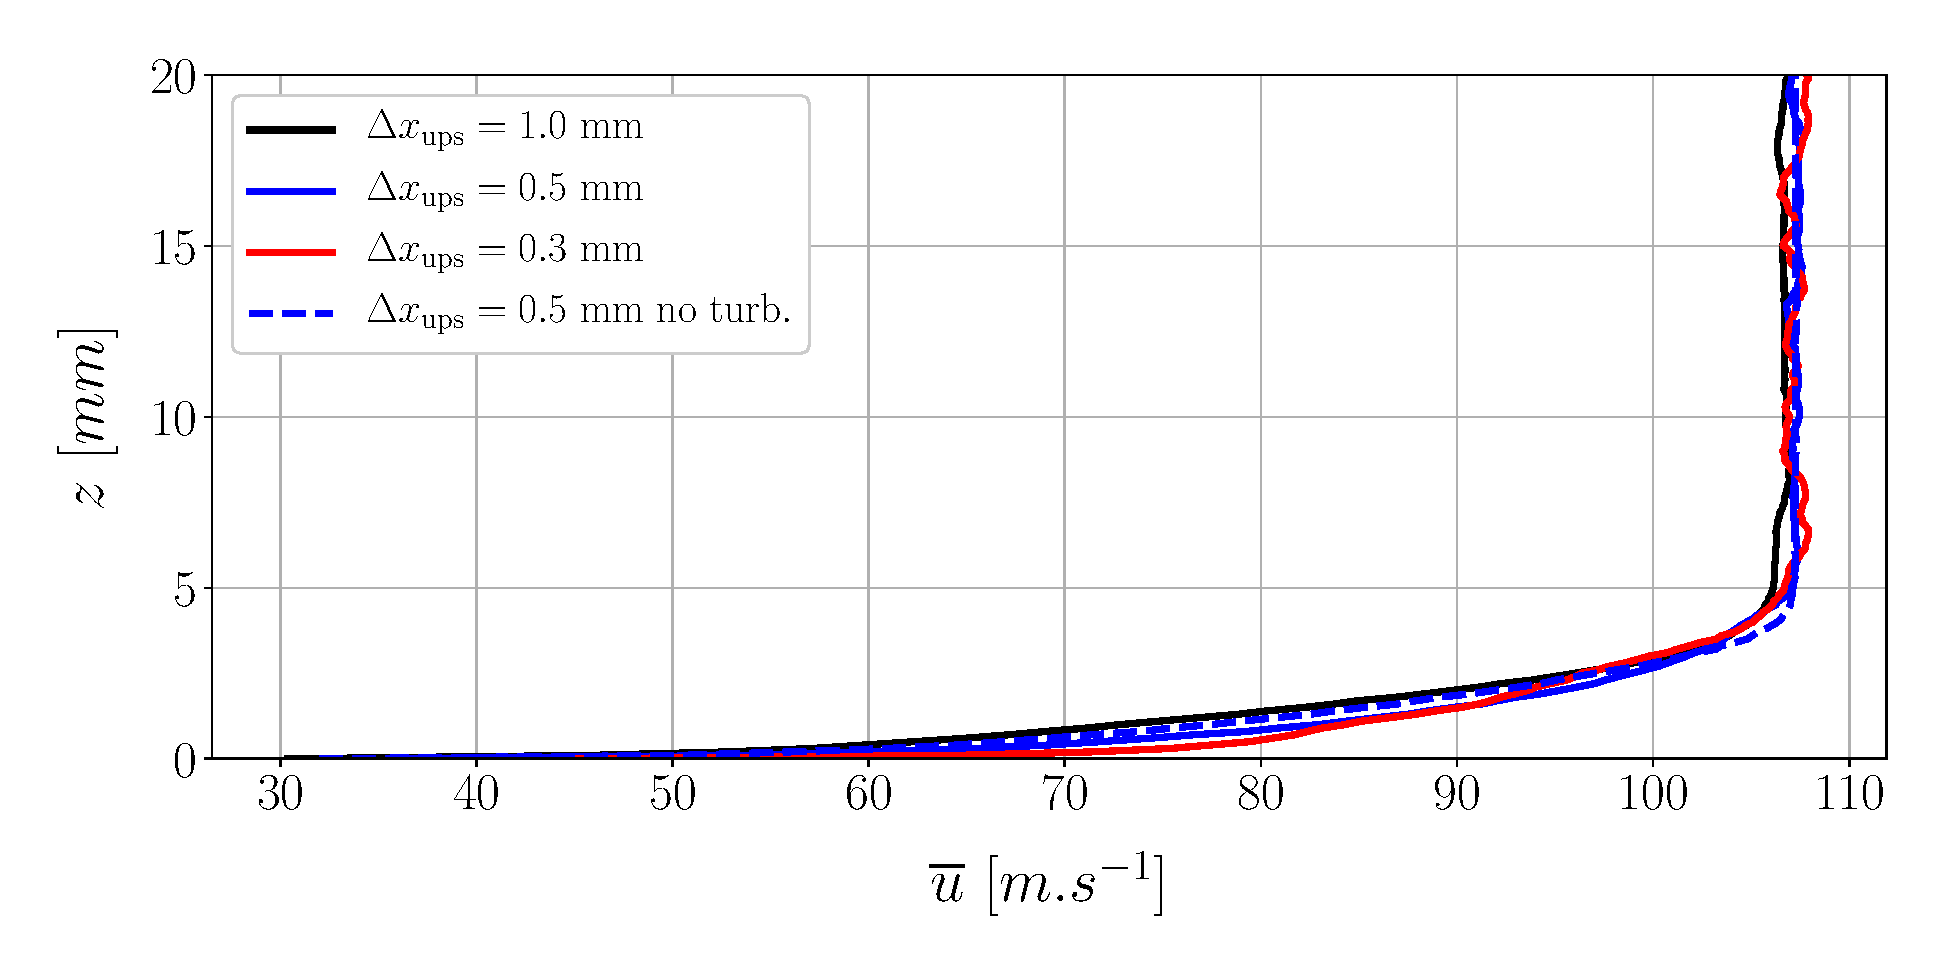
\includegraphics[scale=0.25]{./part2_developments/figures_ch5_resolved_JICF/results_ics_mesh_convergence_mean_profiles/U_MEAN_profiles.pdf}
   \caption{Mean axial velocity}
   %\label{} 
\end{subfigure}
\hfill
\begin{subfigure}[b]{0.45\textwidth}
	\centering
   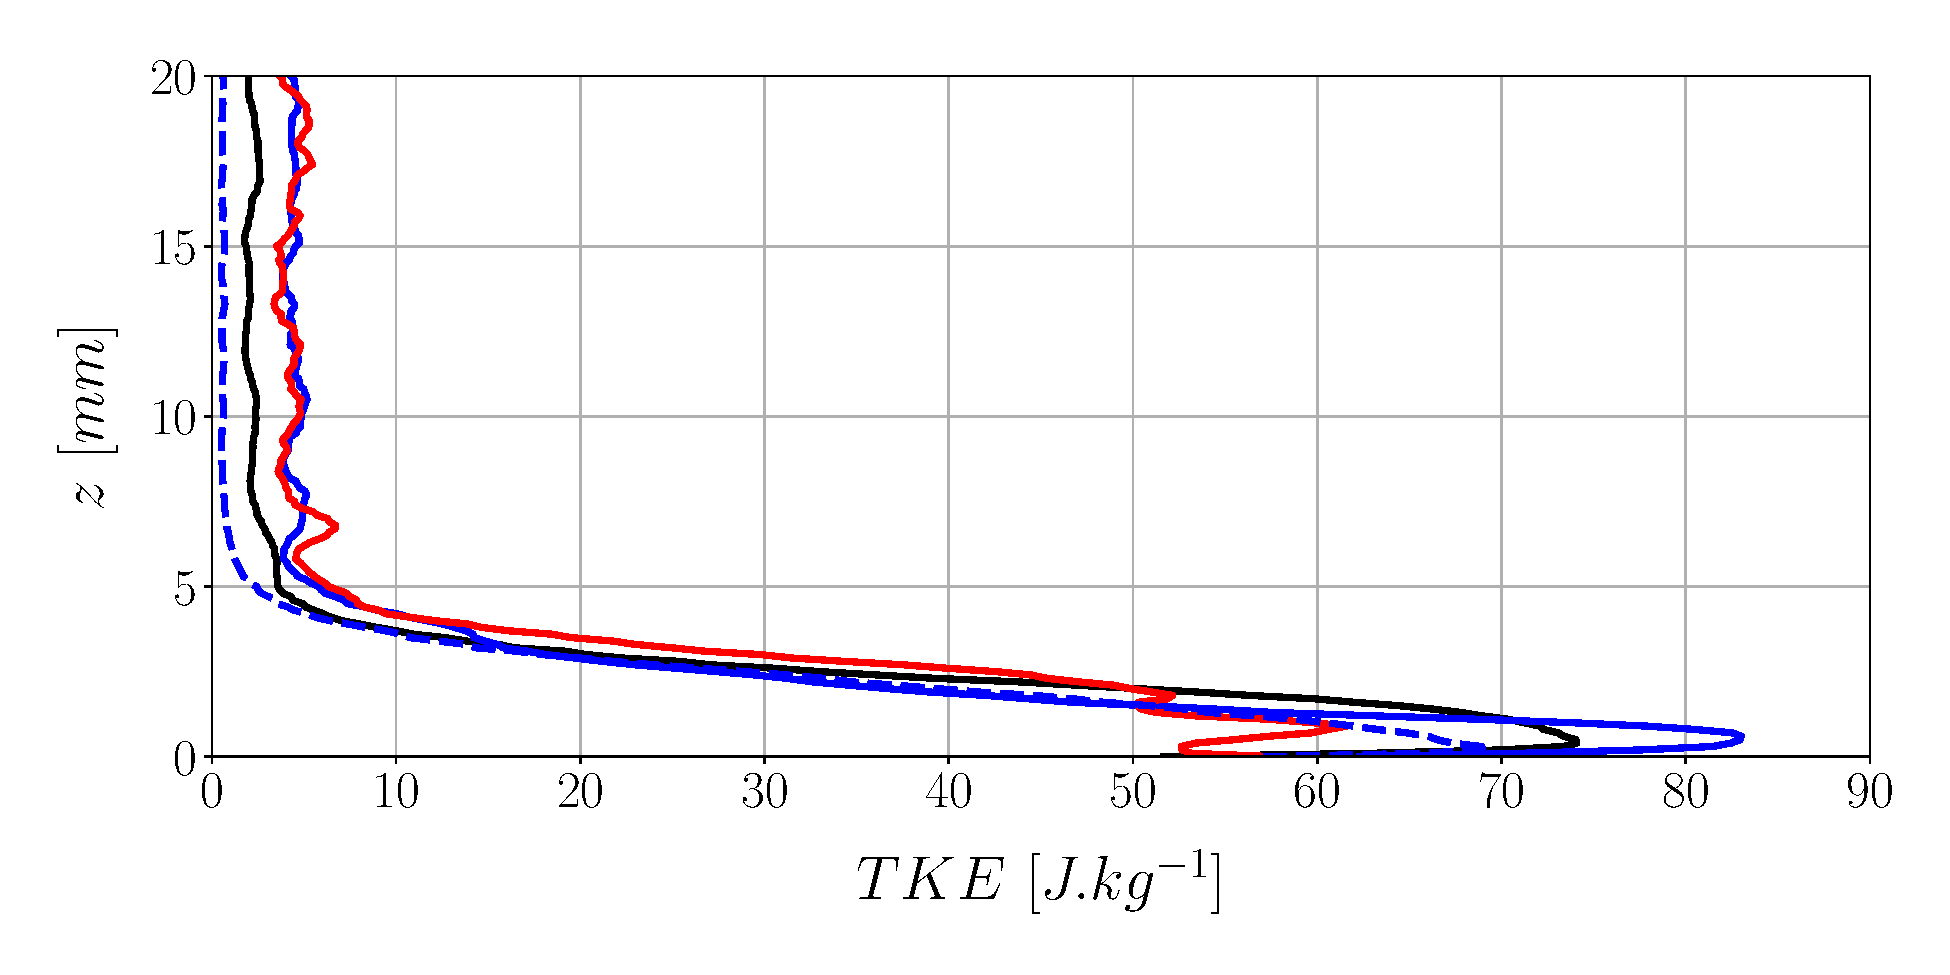
\includegraphics[scale=0.25]{./part2_developments/figures_ch5_resolved_JICF/results_ics_mesh_convergence_mean_profiles/TKE_profiles.pdf}
   \caption{Turbulent Kinetic Energy}
   %\label{}
\end{subfigure}
\caption{Profiles of $\overline{u}$ and $TKE$ along the line right upstream the injector.}
\label{fig:ics_mesh_independency_study_mean_profiles} 
\end{figure}





\begin{figure}[ht]
\centering
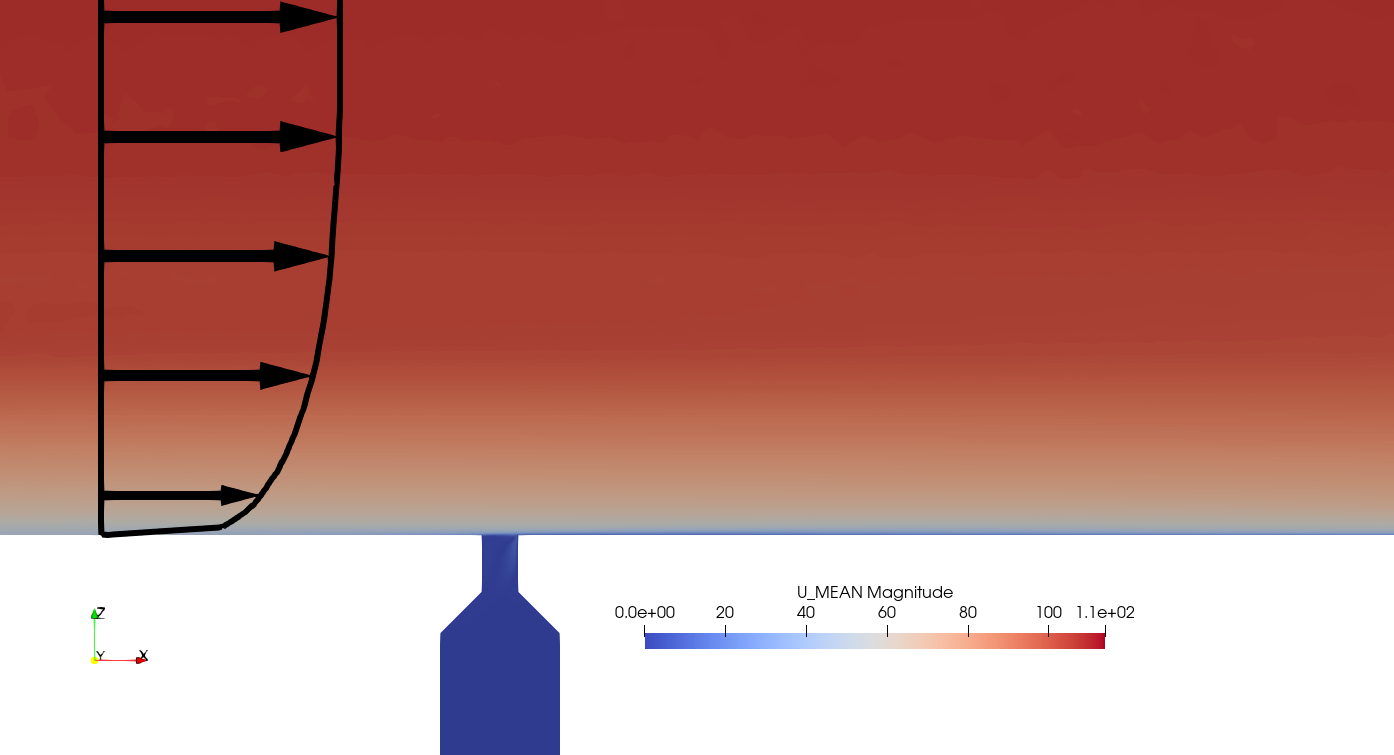
\includegraphics[scale=0.2]{./part2_developments/figures_ch5_resolved_JICF/Umean_profile_with_jet}
\caption{reza}
% OJO: ficheros generados para el perfil de velocidades estan en Ongoing\ICS_study\u_mean_profiles\cases_probes\mesh_refined_DX0p5_ics_no_actuator_flat_BL_with_turbulence_L3p00_up2p7
\label{fig:Umean_profile_with_jet}
\end{figure}




\subsection{Initial conditions for low Weber operating point}

Initial conditions have also obtained for the operating point at lower Weber number ($We_g = 830$) with the mesh resolution $\Delta x_\mathrm{ups} = 0.5$ mm. For establishment of the gaseous phase, the simulation has been run for 40 times the flow-through time shown in Table \ref{tab:jicf_operating_conditions_turbulent_injection_parameters}. This time, which has been checked to profiled converged solutions, has been chosen from the results obtained with the operating point at high We, as shown in Figure \ref{fig:mesh_convergence_line_averages}. Converged profiles for mean axial velocity and $TKE$ are shown in Figure \ref{fig:ics_mean_profiles_op2}, the profiles for the high We operating point are also shown for comparison. As expected, both $\overline{u}$ and $TKE$ values are lower along the $z$ coordinates for the lower We point, consistent with the lower bulk values of $u_\infty$ and $u'$ imposed at the gaseous inletfor this case.

\begin{figure}[ht]
\centering
\begin{subfigure}[b]{0.45\textwidth}
	\centering
   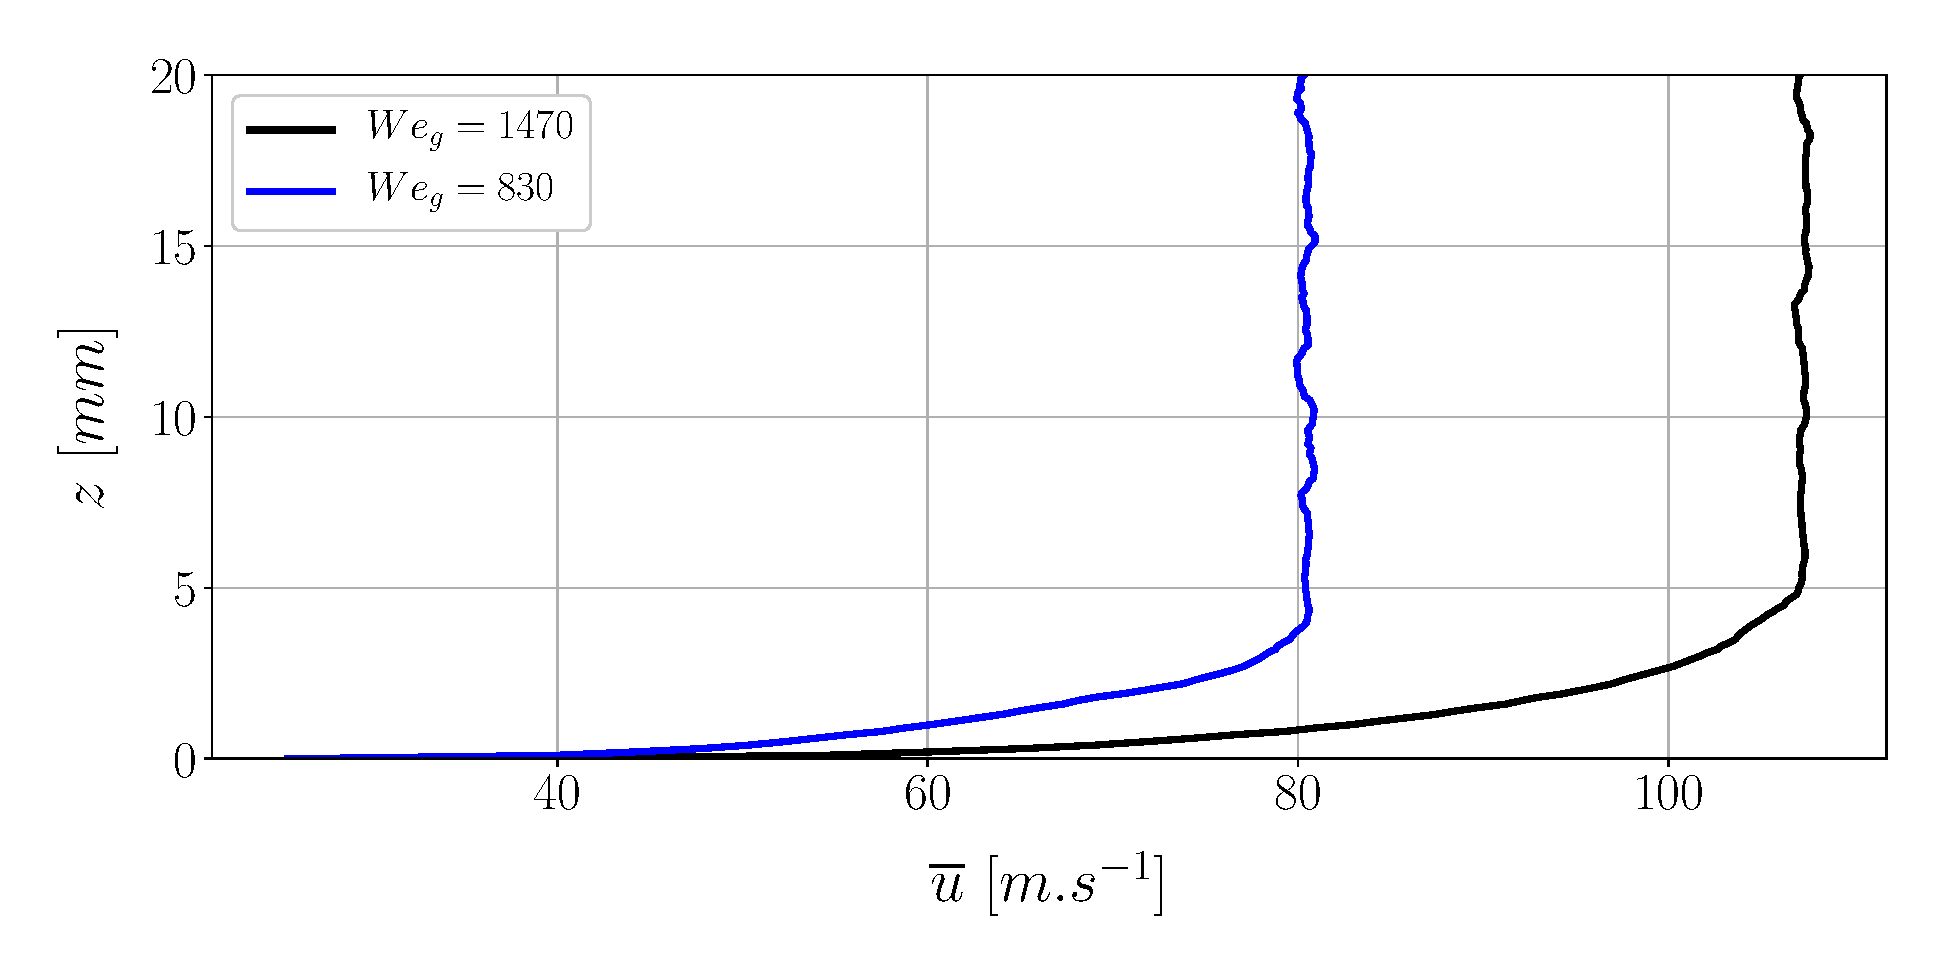
\includegraphics[scale=0.25]{./part2_developments/figures_ch5_resolved_JICF/results_ics_mesh_convergence_mean_profiles/U_MEAN_profiles_op2.pdf}
   \caption{Mean axial velocity}
   %\label{} 
\end{subfigure}
\hfill
\begin{subfigure}[b]{0.45\textwidth}
	\centering
   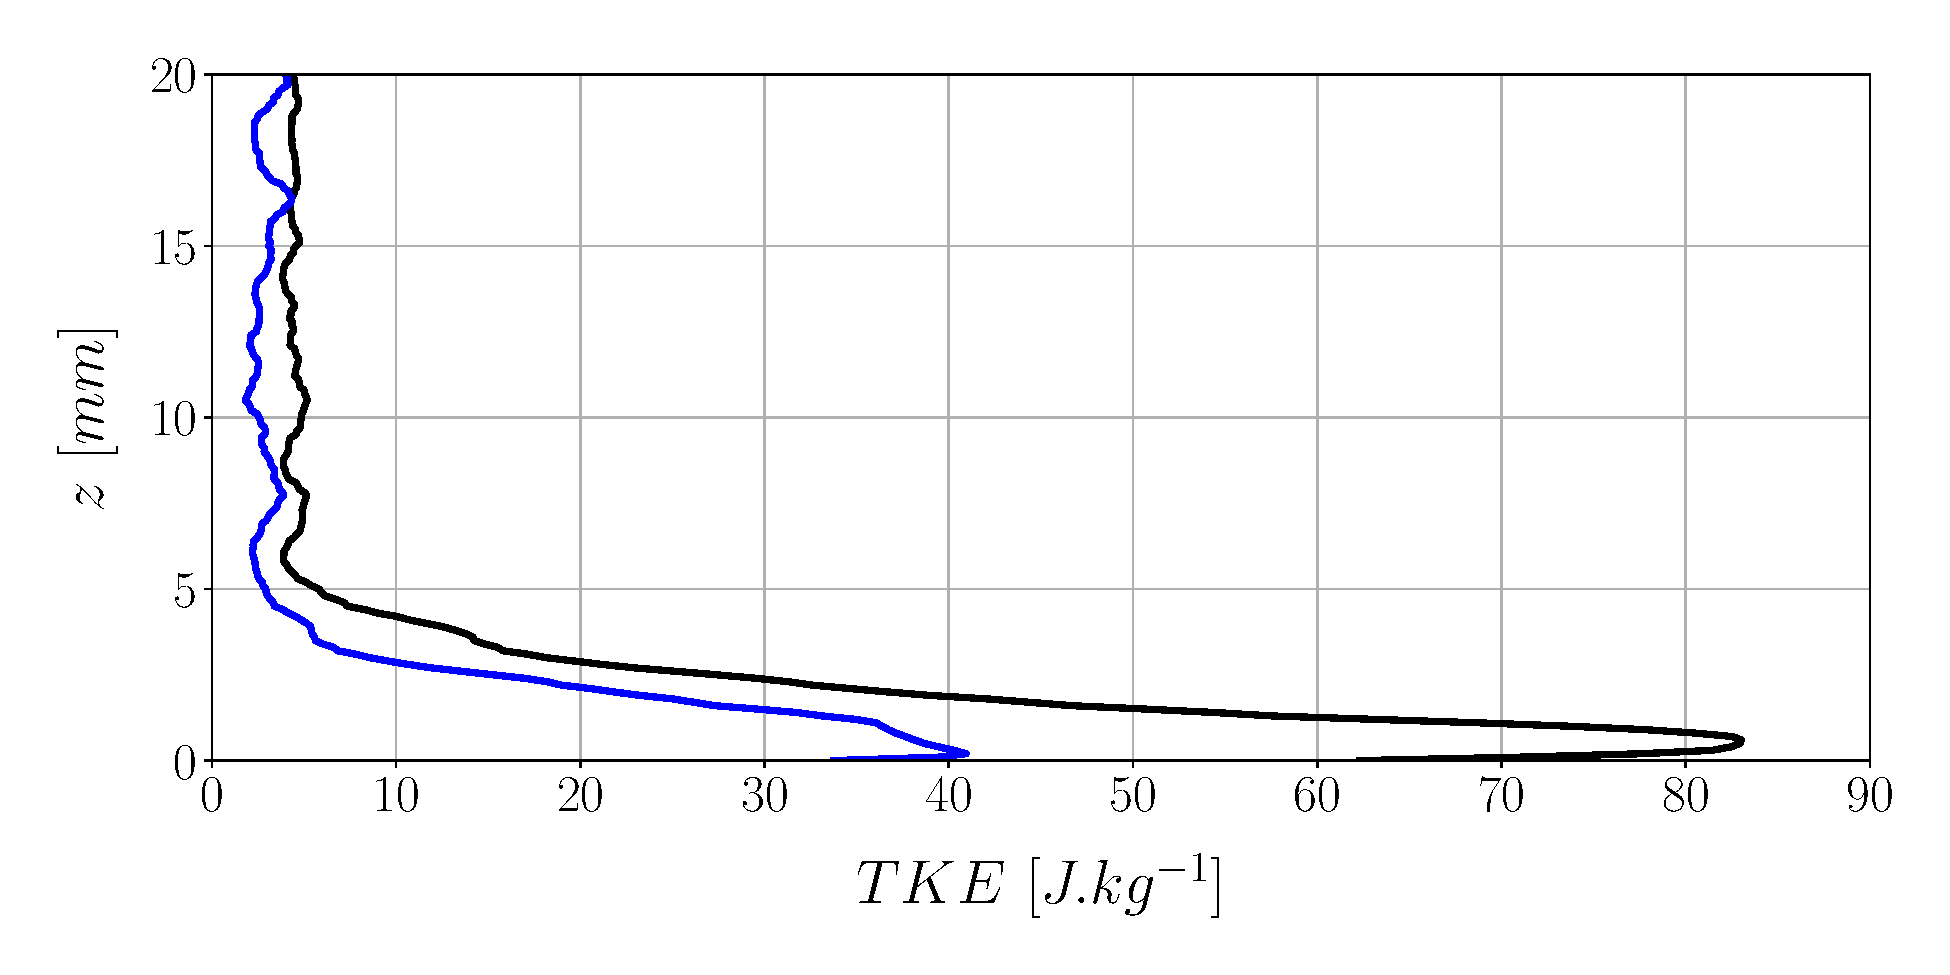
\includegraphics[scale=0.25]{./part2_developments/figures_ch5_resolved_JICF/results_ics_mesh_convergence_mean_profiles/TKE_profiles_op2.pdf}
   \caption{Turbulent Kinetic Energy}
   %\label{}
\end{subfigure}
\caption{Profiles of $\overline{u}$ and $TKE$ along the line right upstream the injector for both operating points for mesh resolution $\Delta x_\mathrm{ups} = 0.5$ mm.}
\label{fig:ics_mean_profiles_op2}
\end{figure}




%\begin{figure}[ht]
%	\centering
%   \includegraphics[scale=0.28]{./part2_developments/figures_ch5_resolved_JICF/results_ics_mesh_convergence_probes/up_OP2.eps}
%   \includegraphics[scale=0.28]{./part2_developments/figures_ch5_resolved_JICF/results_ics_mesh_convergence_probes/spectra_linear_scale_OP2.eps}
%   \caption{Mesh $\Delta x_\mathrm{ups} = 0.5$ mm, low-We operating point}
%   \label{fig:ics_probes_OP2}
%\end{figure}
%



\section{Definition of liquid characteristic times}
\label{sec:ch5_liquid_characteristic_times}

In the previous section, convergence of statistics in gaseous simulations were monitored in time with respect to a characteristic time name flow-through ($\tau_\mathrm{ft}$). Characteristic times are useful since they represent appropriate temporal scales of the physical processes involved in a given problem. The fastest physical mechanisms, given by the smallest characteristic times, will be ones governing each particular case. Also, evolution of statistical quantities can then be monitored by comparing the running times of the simulations with the characteristic times relevant to the magnitudes of interest. 

In the same fashion as in the gaseous simulations, characteristic times can be defined for the liquid phase. Firstly, several characteristic physical times can be mathematically defined for the liquid phase from the physical characteristics of the flow:

\begin{itemize}

	\item Characteristic time related to the \textbf{ inertia of the liquid phase}, $\tau_\mathrm{in}$. This timescale is used in literature to express the establishment of liquid jets in crossflow \citepColor[herrmann_impact_2011].

	\item Characteristic time of \textbf{breakup procresses}. Reference times relating to liquid breakup were firstly introduced by \citeColor[ranger_aerodynamics_1968] to provide an order of magnitude of droplet disintegration in high-velocity gaseous flows. It was later applied to liquid jets in crossflow by \citeColor[fuller_effects_2000], who distinguished two breakup times: an \textbf{aerodynamic breakup timescale} $\tau_\mathrm{ab}$ as defined in \citeColor[ranger_aerodynamics_1968] for droplets since the breakup mechanisms for droplets and jets are similar when aerodynamic forces are significant; and a \textbf{non-aerodynamic timescale} $\tau_\mathrm{nb}$ which is representative of the breakup process when aerodynamic forces are weak.
	
	\item \textbf{Capillary timescale} $\tau_\mathrm{cap}$ \citepColor[eggers_physics_2008].
	
%	\item \textbf{Viscous timescale} $\tau_\mathrm{visc}$ \citepColor[mckinley_dimensionless_2005].
	


\end{itemize}

\begin{table}[!h]
\centering
\caption{Characteristic physical timescales [$\mu$s] in JICF simulations}
\begin{tabular}{cccc}
\thickhline
\textbf{Time scale} & \textbf{Expression} & \textbf{Low Weber} & \textbf{High Weber} \\
\thickhline
Inertia & $\tau_\mathrm{in} = \frac{d_\mathrm{inj}}{u_l}$ & 25.72 & 19.29 \\
Aerodynamic breakup  &  $\tau_\mathrm{ab} =  \frac{d_\mathrm{inj}}{u_g - u_l} \sqrt{\frac{\rho_l}{\rho_g}} $ & 82.17 & 61.63 \\
Non-aerodynamic breakup  &  $\tau_\mathrm{nb} = \frac{d_\mathrm{inj}}{u_l} We_l^{1/3} $ &  439.16 & 339.00 \\
Capillary & $\tau_\mathrm{cap} = \sqrt{\frac{\rho_l d_\mathrm{inj}^3}{8 \sigma}}$ & 1814.64 & 1814.64 \\
%Viscous & $\tau_\mathrm{visc} = \frac{\mu_l d_\mathrm{inj}}{\sigma}$ & & \\
\thickhline
\end{tabular}
\label{tab:jicf_characteristic times}
\end{table}


These characteristic times are defined and calculated for each simulation in Table \ref{tab:jicf_characteristic times}. As observed, all timescales are lower for the high Weber operating point due to the higher velocities involved in this case (except for the capillary one, which does not depend on the flow conditions). The capillary timescale is larger than the other ones due to the strong aerodynamic conditions found in both operating points: capillary events are slow and do not contribute to the jet development and breakup, which are governed by inertia. Regarding breakup timescales, aerodynamic breakup is faster relative to non-aerodynamic in both cases, indicating that aerodynamic effect prevails: effectively, the main primary atomization mechanism governing both operating points is surface breakup, as indicated in Figure \ref{fig:location_JICF_ops_in_breakup_map}. In this work, the only reference time that will be further used is the inertia timescale $\tau_\mathrm{in}$ to express the jet establishment in a dimensionless timescale and allow a qualitative comparison of both operating points. 

Secondly, characteristic times can also be obtained directly from the simulations performed. These ones cannot be directly estimated through expressions, but are obtained by postprocessing results of interest in the simulations. They are useful for expressing the evolution and convergence of statistical quantities studied. Contrarily to the first set of timescales defined previously, which are obtained through expressions and therefore do not depend on the mesh resolution, \hl{the characteristic times obtained from the simulations are dependent on both the operating point and the mesh resolution}. In this work, two timescales are used: 

\begin{itemize}

	\item  Characteristic times of the \textbf{ligaments stripping from the dense core} in resolved simulations, $\tau_\mathrm{str}$. This value is obtained by counting the number of liquid structures that emanate from the liquid column in a given time period.

	
	\item \textbf{Characteristic droplet arrival times} to the sampling planes in the simulations. They are obtained as the elapsed time from the initialisation of the two-phase simulation to the arrival of the first droplet to each sampling plane. As several sampling planes are defined in each simulation (see for example Figure \ref{fig:jicf_interior_boundaries_surface_measurements}), several sampling timescales are obtained. Results are shown in Table \ref{tab:jicf_characteristic_droplet_sampling_times}. The justification for the choice of sampling planes is done in $\S$\ref{ref:ch5_sec_spray_characterization}.


\end{itemize}



\begin{table}[!h]
\centering
\caption{Characteristic droplet arrival times to sampling planes $\tau_\mathrm{dr_x}$ [$\mu$s] in JICF simulations}
\begin{tabular}{ccccc}
\thickhline
\textbf{Case} & $x = 5$ mm & $x = 10$ mm & $x = 15$ mm  \\
\thickhline 
UG75\_DX10  & 192.7 & 295.2 & -  \\
UG75\_DX20  & 234.7 & 355.8 & 456.7 \\
UG100\_DX10 & 143.7 & 218.7 & - \\
UG100\_DX20 & 176.8 & 258.4 & 362.8 \\
\thickhline
\end{tabular}
\label{tab:jicf_characteristic_droplet_sampling_times}
\end{table}


%\section{Results}
%\label{sec:results_JICF_resolved}

\section{Jet evolution}


\subsection{Flow establishment}
\label{subsec:ch5_JICF_flow_establishment}

Figures \ref{fig:JICF_establishment_UG100_lateral} to \ref{fig:JICF_establishment_UG75_top} shows the evolution of the jet for all the simulations in three different view: lateral, front and top. The left column shows the thicker resolution, while the right column shows the finer one. The interface is represented by the iso-value $\Psi = 0.5$. The snapshots are represented for the same time instants in all cases, which are expressed in dimensionless units with respect to the characteristic liquid inertia timescale introduced in Table \ref{tab:jicf_characteristic times}:

\begin{equation}
t^* = \frac{t}{\tau_\mathrm{in}}
\end{equation}

Note that $\tau_\mathrm{in}$ is, due to its definition, higher for the low-We operating point than for the high-We one. Therefore, the absolute times from injection are not the same for both operating points: for the same time instant $t^*$, the low-We point represents a more advanced physical time than the high-We case. This allows to compare the jets at equivalent times: since the low-We operating point involves lower gas and liquid velocities, the jet has advanced in a lesser extent than the high-We case for the same absolute time instant. Therefore, expressing a dimensionless time with respect to a reference time that takes into account the difference in velocity between both cases (in this case, the one of the liquid phase) allows for a more representative comparison of both jets.

The lateral view of the jets (Figures \ref{fig:JICF_establishment_UG100_lateral} and \ref{fig:JICF_establishment_UG75_lateral}) show 

No difference in penetration can be observed \ref{subsec:ch5_jet_trajectories_results}.


\clearpage

\begin{figure}[ht]
\centering
\includeinkscape[inkscapelatex=false,scale=0.8]{./part2_developments/figures_ch5_resolved_JICF/JICF_establishment_UG100_lateral}
\caption[Lateral view of high We jet at several time instants. ]{Lateral view of high We jet at several time instants. \textsl{Left}: UG100\_DX20. \textsl{Right}: UG100\_DX10.}
\label{fig:JICF_establishment_UG100_lateral}
\end{figure}

\clearpage

\begin{figure}[ht]
\centering
\includeinkscape[inkscapelatex=false,scale=0.8]{./part2_developments/figures_ch5_resolved_JICF/JICF_establishment_UG100_front}
\caption[Front view of high We jet at several time instants. ]{Front view of high We jet at several time instants. \textsl{Left}: UG100\_DX20. \textsl{Right}: UG100\_DX10.}
\label{fig:JICF_establishment_UG100_front}
\end{figure}
\clearpage

\clearpage

\begin{figure}[ht]
\centering
\includeinkscape[inkscapelatex=false,scale=0.8]{./part2_developments/figures_ch5_resolved_JICF/JICF_establishment_UG100_top}
\caption[Top view of high We jet at several time instants. ]{Top view of high We jet at several time instants. \textsl{Left}: UG100\_DX20. \textsl{Right}: UG100\_DX10.}
\label{fig:JICF_establishment_UG100_top}
\end{figure}




\clearpage

\begin{figure}[ht]
\centering
\includeinkscape[inkscapelatex=false,scale=0.8]{./part2_developments/figures_ch5_resolved_JICF/JICF_establishment_UG75_lateral}
\caption[Lateral view of low We jet at several time instants. ]{Lateral view of low We jet at several time instants. \textsl{Left}: UG75\_DX20. \textsl{Right}: UG75\_DX10.}
\label{fig:JICF_establishment_UG75_lateral}
\end{figure}

\clearpage

\begin{figure}[ht]
\centering
\includeinkscape[inkscapelatex=false,scale=0.8]{./part2_developments/figures_ch5_resolved_JICF/JICF_establishment_UG75_front}
\caption[Front view of low We jet at several time instants. ]{Front view of low We jet at several time instants. \textsl{Left}: UG75\_DX20. \textsl{Right}: UG75\_DX10.}
\label{fig:JICF_establishment_UG75_front}
\end{figure}

\clearpage

\begin{figure}[ht]
\centering
\includeinkscape[inkscapelatex=false,scale=0.8]{./part2_developments/figures_ch5_resolved_JICF/JICF_establishment_UG75_top}
\caption[Top view of low We jet at several time instants. ]{Top view of low We jet at several time instants. \textsl{Left}: UG75\_DX20. \textsl{Right}: UG75\_DX10.}
\label{fig:JICF_establishment_UG75_top}
\end{figure}

\clearpage

\subsection{Breakup topology}

Things break yes.

\subsection{Presence of instabilities / instabilities resolution}
\label{subsec:ch5_instabilities_presence}

Instabilities present for the fine resolution but not for the coarse one.

We can look at the \textbf{vorticity}. We can also look within the \textbf{liquid injector}.

As observed in Figure \textbf{XX}, ligaments generated due to instabilities in the fine resolution simulations \hl{contain a higher inertia and are stripped-off the dense core with larger velocities than those produced in the coarse resolution, where instabilities are not generated}. Such ligaments and the subsequent droplets produced from their breakup will penetrate further away in the vertical direction.

We can see in Figure \textbf{XX} that the wavelengths $\lambda$ of the generated instabilities are ...

When instabilities are present, primary atomization is affected and the generated ligaments \hl{contain more inertia}. As


\subsection{Evolution of mesh size}

At the early instants of the injection process, the quantity of liquid in the domain increases with time until the jet is established. Since dynamic mesh adaptation is used to locate the smallest mesh elements in the liquid-gas interface (as explained in $\S$\ref{subsec:ch2_ACLS}), the mesh size increases with time as the interface surface within the domain is larger. 

\begin{figure}[ht]
\centering
	\centering
   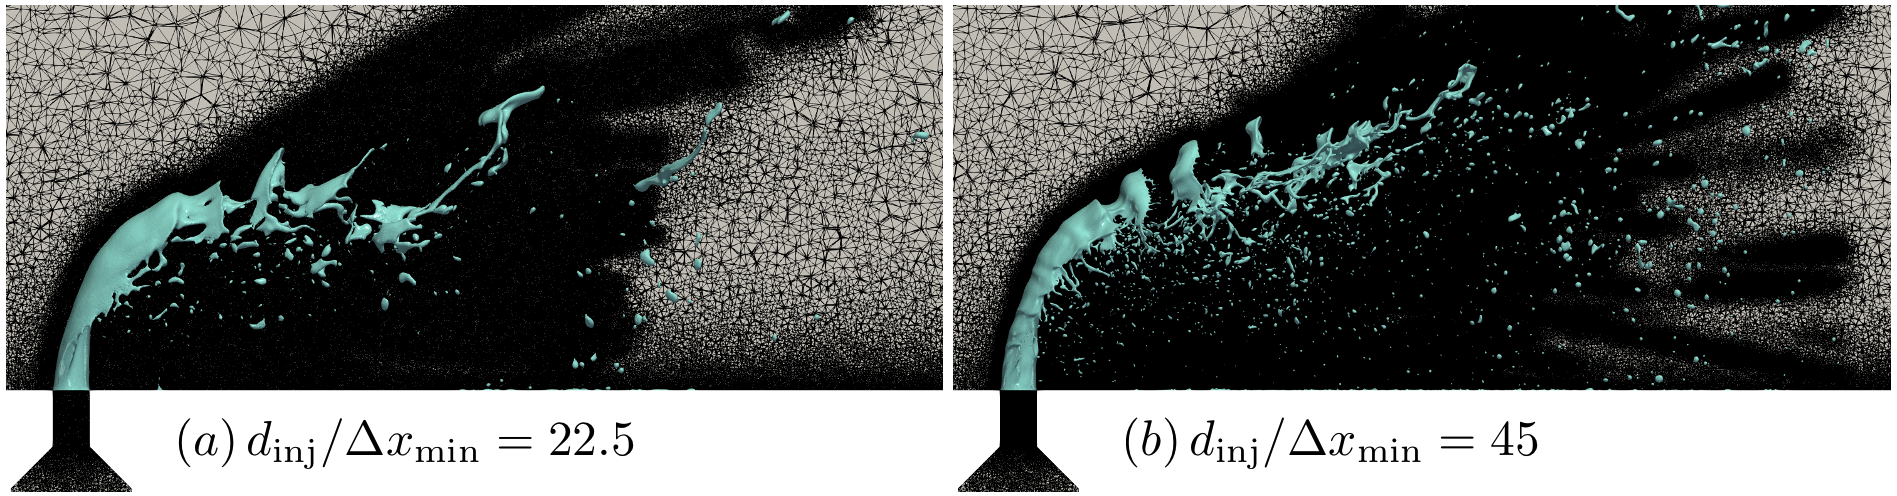
\includegraphics[scale=0.25]{./part2_developments/figures_ch5_resolved_JICF/JICF_nelem_evolution/JICF_w_mesh}
   %\label{} 
\caption{Lateral view of meshes and interface contours near the injector at time instant t = 0.3 ms, high Weber point}
\label{fig:JICF_w_mesh}
\end{figure}

The evolution of the number of mesh elements ($N_\mathrm{elements}$) with time in all simulations is shown in Figure \ref{fig:JICF_nelem_increase}. In this case, the physical time has been expressed with respect to the arrival time of the first droplet to the last sampling plane before liquid is removed, $\tau_\mathrm{dr_{xLast}}$, which are shown in Table \ref{tab:jicf_characteristic_droplet_sampling_times}:

\begin{equation}
t^{\prime} = \frac{t}{\tau_\mathrm{dr_{xLast}}}
\end{equation}

Note that the last sampling plane differs on the mesh resolution: for $\Delta x_\mathrm{min} = 20~\mu m$ is at $x = 15$ mm, while for $\Delta x_\mathrm{min} = 10~\mu m$ is at $x = 10$ mm. For the fine resolution liquid is artificially removed before than in the coarse one because the cost of the simulations was shown to be too expensive if droplets are present up to $15$ mm downstream the injection nozzle. Therefore, the final values of the number of elements (i.e. once the jet is established) are not directly comparable between resolutions, but only between operating point. However, a quick glance to Figure \ref{fig:JICF_nelem_increase_all_t} shows that, despite liquid being suppressed upstream than in the fine resolution, the final number of elements is larger in the former than in the later: \textsl{(add numbers when simulations are stable)}. By looking at Figure \ref{fig:JICF_nelem_increase_all_t}, one can see that the number of elements increases slowly at the beginning and then rises exponentially (linearly in the semi-logarithmic plot) \hl{until there's enough liquid in the domain} and steady-state is reached. The number of elements is much larger for the fine resolution tan for the coarse one: \hl{the steady-state values are ...}. \\

\textbf{ALTERNATIVE} The evolution of the number of mesh elements ($N_\mathrm{elements}$) with time in all simulations is shown in Figure \ref{fig:JICF_nelem_increase}. In this case, the physical time has been expressed with respect to the arrival time of the first droplet to the sampling plane at $x = 10$ mm, $\tau_\mathrm{dr_{x=10}}$ , which are shown in Table \ref{tab:jicf_characteristic_droplet_sampling_times}:



\begin{equation}
\label{eq:t_prime_with_tau_drx10}
t^{\prime} = \frac{t}{\tau_\mathrm{dr_{x=10}}}
\end{equation}

The plane $x = 10$ mm has been chosen because it is the last plane where liquid is sampled before being artificially removed in the fine simulations with $\Delta x_\mathrm{min} = 10 ~\mu m$. For the coarse resolution $20 ~\mu m$, liquid is removed after $x = 15$ mm. Yet, dimensionless time is expressed with respect to the time corresponding to plane $x = 10$ mm in order to compare between cases. Figure \ref{fig:JICF_nelem_increase}a shows the increase in number of elements with respect to dimensionless simulation time. It is shown that, despite liquid being suppressed upstream in the fine resolution, the final number of elements is larger in the former than in the later: (add numbers when simulations are stable). By looking at Figure \ref{fig:JICF_nelem_increase}a, one can see that the number of elements increases slowly at the beginning and then rises exponentially (linearly in the semi-logarithmic plot) until there’s \hl{enough liquid in the domain} and steady-state is reached. The number of elements is much larger for the fine resolution than for the coarse one: \hl{the steady-state values are ... }

The dashed line in Figures \ref{fig:JICF_nelem_increase_all_t} and  \ref{fig:JICF_nelem_increase_t_0_to_2} corresponds  to $t^{\prime} = 1$, which is the instant at which the last sampling plane in each simulation detects the first droplet. Figure \ref{fig:JICF_nelem_increase_t_0_to_2} shows that this instant is located in the linear region. Previously, there is no liquid being artificially removed in the simulations, so the curves increase monotonically (except for some minor decreases due to small droplets that reach the size of mesh resolution and disappear due to the unability of being further propagated in the simulations, which is discussed in $\S$\ref{subsec:ch5_mass_conservation_ACLS_set_levelset_band}). After this point, the number of elements continues to increase exponentially up to a time $t^{\prime} \sim 1.5$ when the derivative starts to decrease and, finally, the number of elements  stabilizes. Right after $t^{\prime} \sim 1.5$ liquid droplets reaching the articifial sponge layer are removed; nevertheless, at this stage there are more droplets being generated in the near-nozzle region due to the disturbance effect of the liquid dense core in the air, which creates turbulence in the gaseous phase that will break ligaments ejected from the dense core into more droplets. This explains the monotonic increase in the number of elements for $t^{\prime} > 1$ until an instant from which the number of elements remains constant, which depends on each simulation. The only noticeable difference at $t^{\prime} = 1$ is for the simulation UG75$\_$DX10, which shows a considerable decrease. \hl{Two reasons might explain this decrease. First, there are not one, but several reaching the last sampling plane, hence these droplets are all removed at the same time from the simulation. Since the mean diameter of the droplets generated in a liquid JICF is larger when the air dynamic pressure is lower} \citepColor[becker_breakup_2002] \hl{, which is the case for the low Weber operating point, the droplets generated in this case are in general lower than for the high Weber case (this is later shown in }$\S$\ref{sec:ch5_sec_spray_characterization}, \hl{, so all these droplets contain more elements than one single droplet from the case } UG75*\_*DX10 \hl{and the removed amount liquid is larger, hence the abrupt decrease in the number of mesh elements. The second explanation could be that at this time instant there are several droplets in the whole domain of the simulation (i.e. from the injection nozzle to the sponge layer location) which disappear at the same time, causing an overall decrease in the number of elements. The combination of both could also occur, which combined would suppose a larger decrease in the number of elements than if every single one acts separately.}

Figure \ref{fig:JICF_nelem_increase_t_0_to_0p5} shows the evolution of number of elements in the black rectangle of Figure \ref{fig:JICF_nelem_increase_t_0_to_2}, which correspond to the early instants of injection. It is seen that for $t^{\prime} \in [0, 0.3]$ the increase in mesh size is slow, but yet the simulations with fine resolutions start to generate more elements than the coarse ones. In this regions, there is no significant difference between operating points. For $t^{\prime} > [0, 0.3]$ the curves start to further differ due to the beginning of atomization: generation of ligaments due to column breakup and of droplets due to surface breakup increase greatly the amount of liquid-gas interface, hence pronouncing the differences in number of mesh elements between resolutions. At this point the effect of the operating points can be noticed: the high Weber case presents a slighly larger number of elements than the low Weber case for both resolutions, as expected since for the former case the aerodynamic forces are stronger and the number of generated droplets is larger (verified in $\S$\ref{subsec:ch5_mass_conservation_ACLS_set_levelset_band})).

The exponential region is observed by looking at the blue rectangle from Figure \ref{fig:JICF_nelem_increase_t_0_to_2}, shown in Figure \ref{fig:JICF_nelem_increase_t_0p5_to_0p7}. This is only a portion of the exponential region, but a representative one since no abrupt decreases in the number of elements due to liquid disappearance are observed. In this graph, it can first be observed that the evolution of element number is not literally monotically increasing, but presents a stepped signal. This is due to the dynamic mesh adaptation routine explained in $\S$\ref{subsec:ch2_ACLS}, which modifies the mesh after a given simulation iterations have passed and not at each iteration: therefore, for some iterations of the simulation $N_\mathrm{elements}$ stay constant. The exponential increase in $N_\mathrm{elements}$ in this region, which is depicted as a linear curve in Figure \ref{fig:JICF_nelem_increase_t_0p5_to_0p7} since the $y$ axis is in logarithmic units, can be fit to an expression relating both magnitudes as follows:

\begin{equation}
N_\mathrm{elements} = n \exp \left( m t^{\prime} \right)
\end{equation}

where $n$ is the $y$-axis intercept and $m$ is the slope. The intercept will be different in all cases; however, the slopes have been found to be different between resolutions but equal between operating points. Therefore two slopes are calculated: $m_{\Delta x10}$ for the fine resolution and $m_{\Delta x20}$ for the coarse one, displayed by the dash-dotted lines in Figure \ref{fig:JICF_nelem_increase_t_0p5_to_0p7}. These slopes have been found to be $m_{\Delta x10} = 3.15$ and $m_{\Delta x20} = 1.6$. \hl{What else ?}

 

\begin{figure}[ht]
\flushleft
\begin{subfigure}[b]{0.45\textwidth}
	\centering
   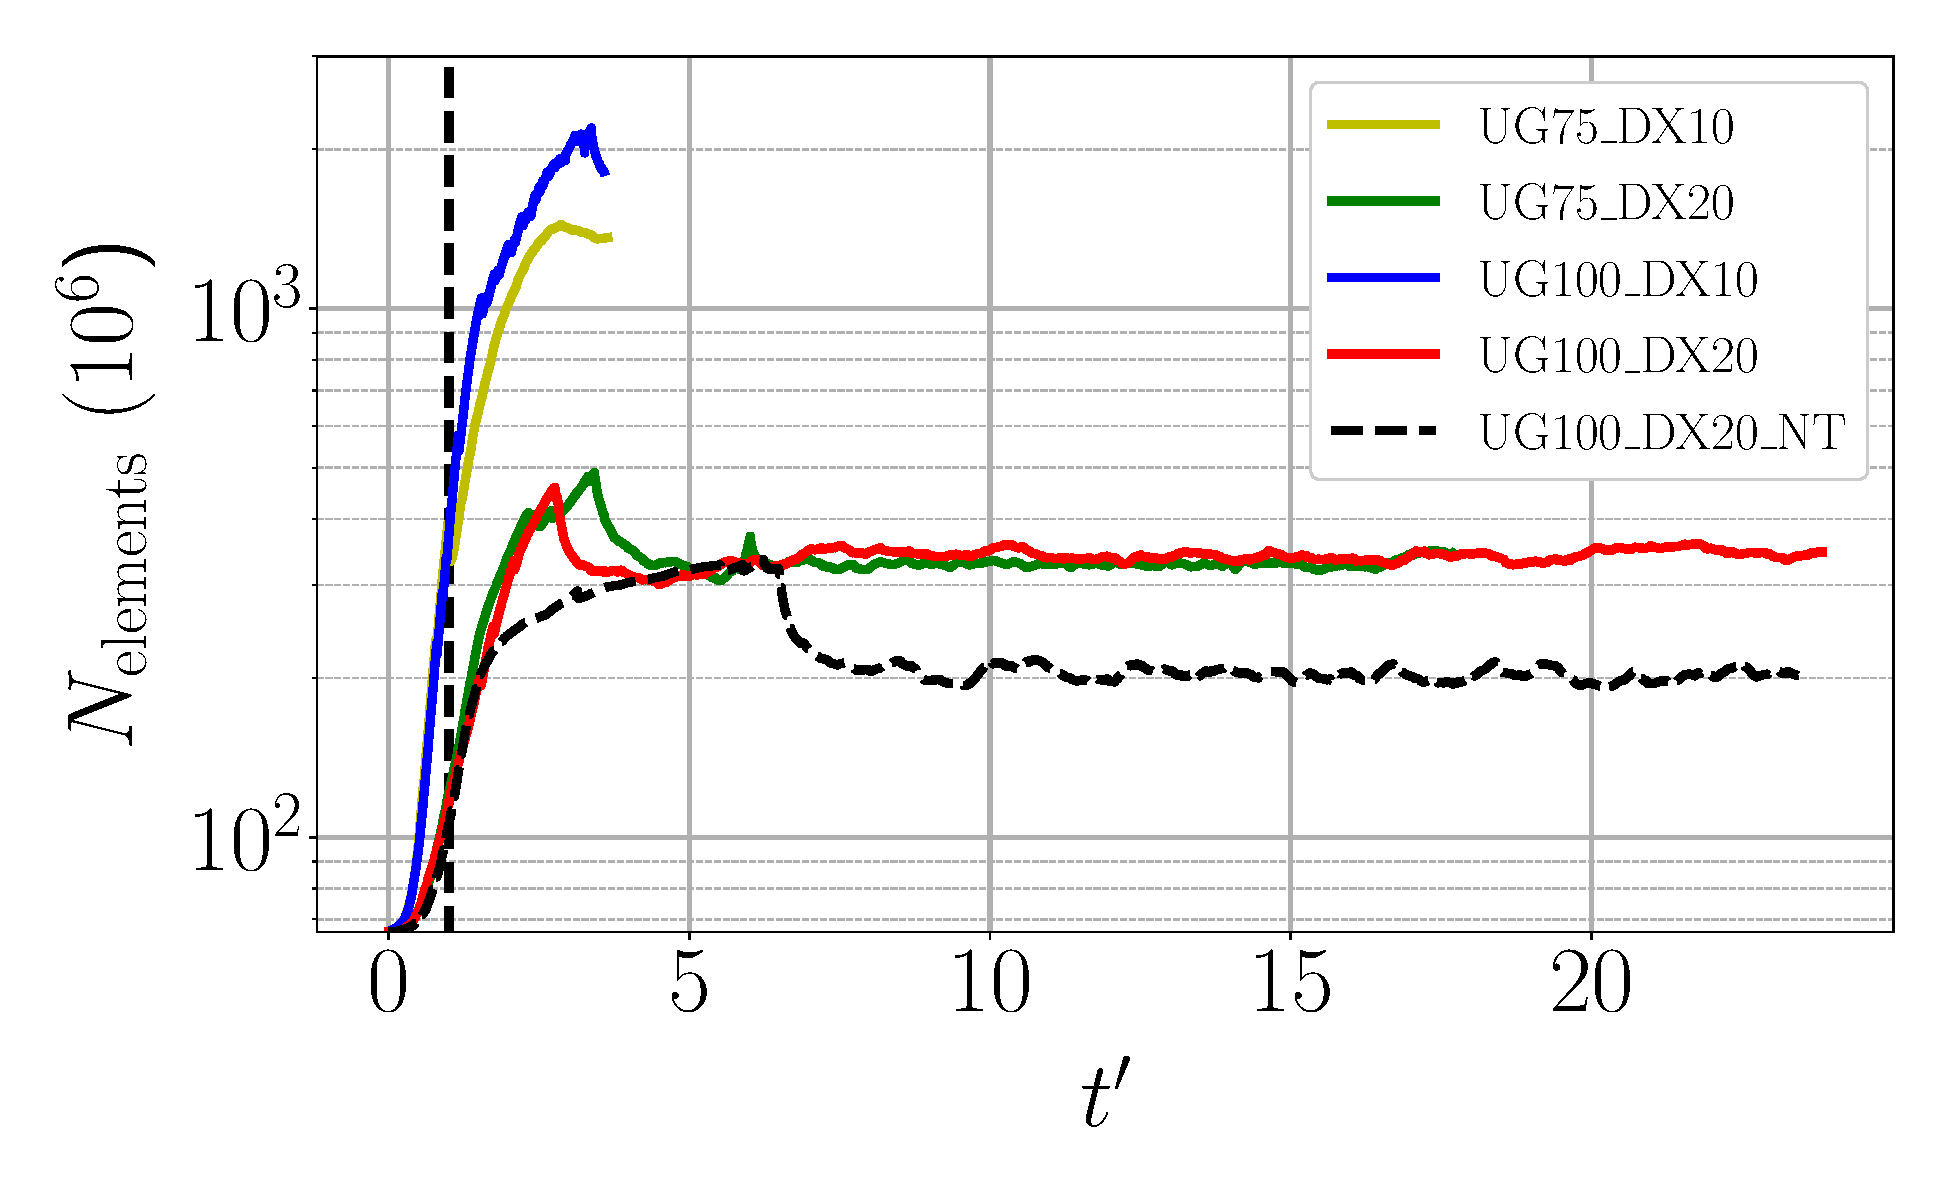
\includegraphics[scale=0.25]{./part2_developments/figures_ch5_resolved_JICF/JICF_nelem_evolution/JICF_nelem_increase}
   \caption{Evolution in simulations}
   \label{fig:JICF_nelem_increase_all_t} 
\end{subfigure}
\hfill
\begin{subfigure}[b]{0.45\textwidth}
	\centering
   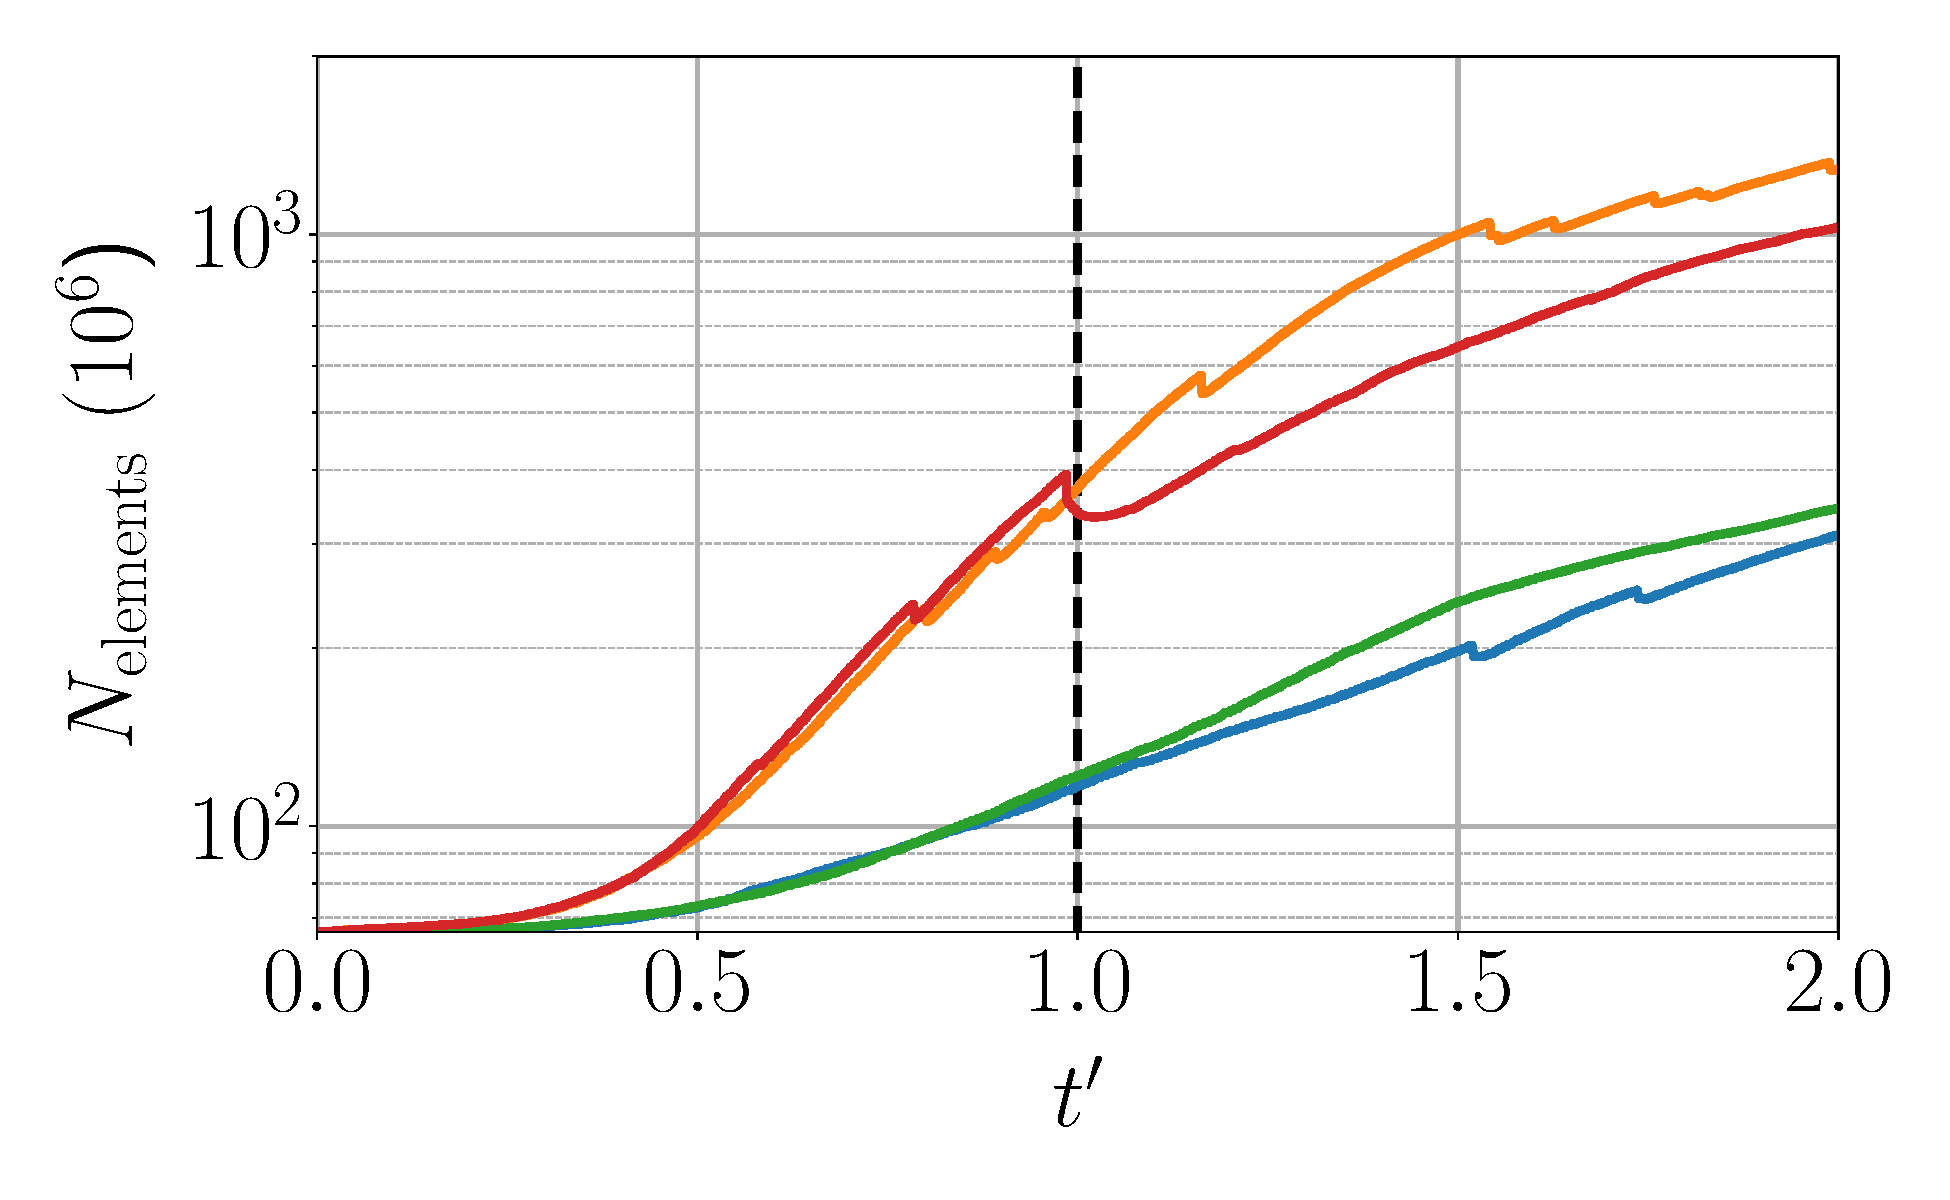
\includegraphics[scale=0.25]{./part2_developments/figures_ch5_resolved_JICF/JICF_nelem_evolution/JICF_nelem_increase_t_in_0_2}
   \caption{Zoomed-in view of Figure \ref{fig:JICF_nelem_increase_all_t} in range $t^{\prime} \in [0, 2]$}
   \label{fig:JICF_nelem_increase_t_0_to_2}
\end{subfigure}

\vskip\baselineskip

\begin{subfigure}[b]{0.45\textwidth}
	\centering
   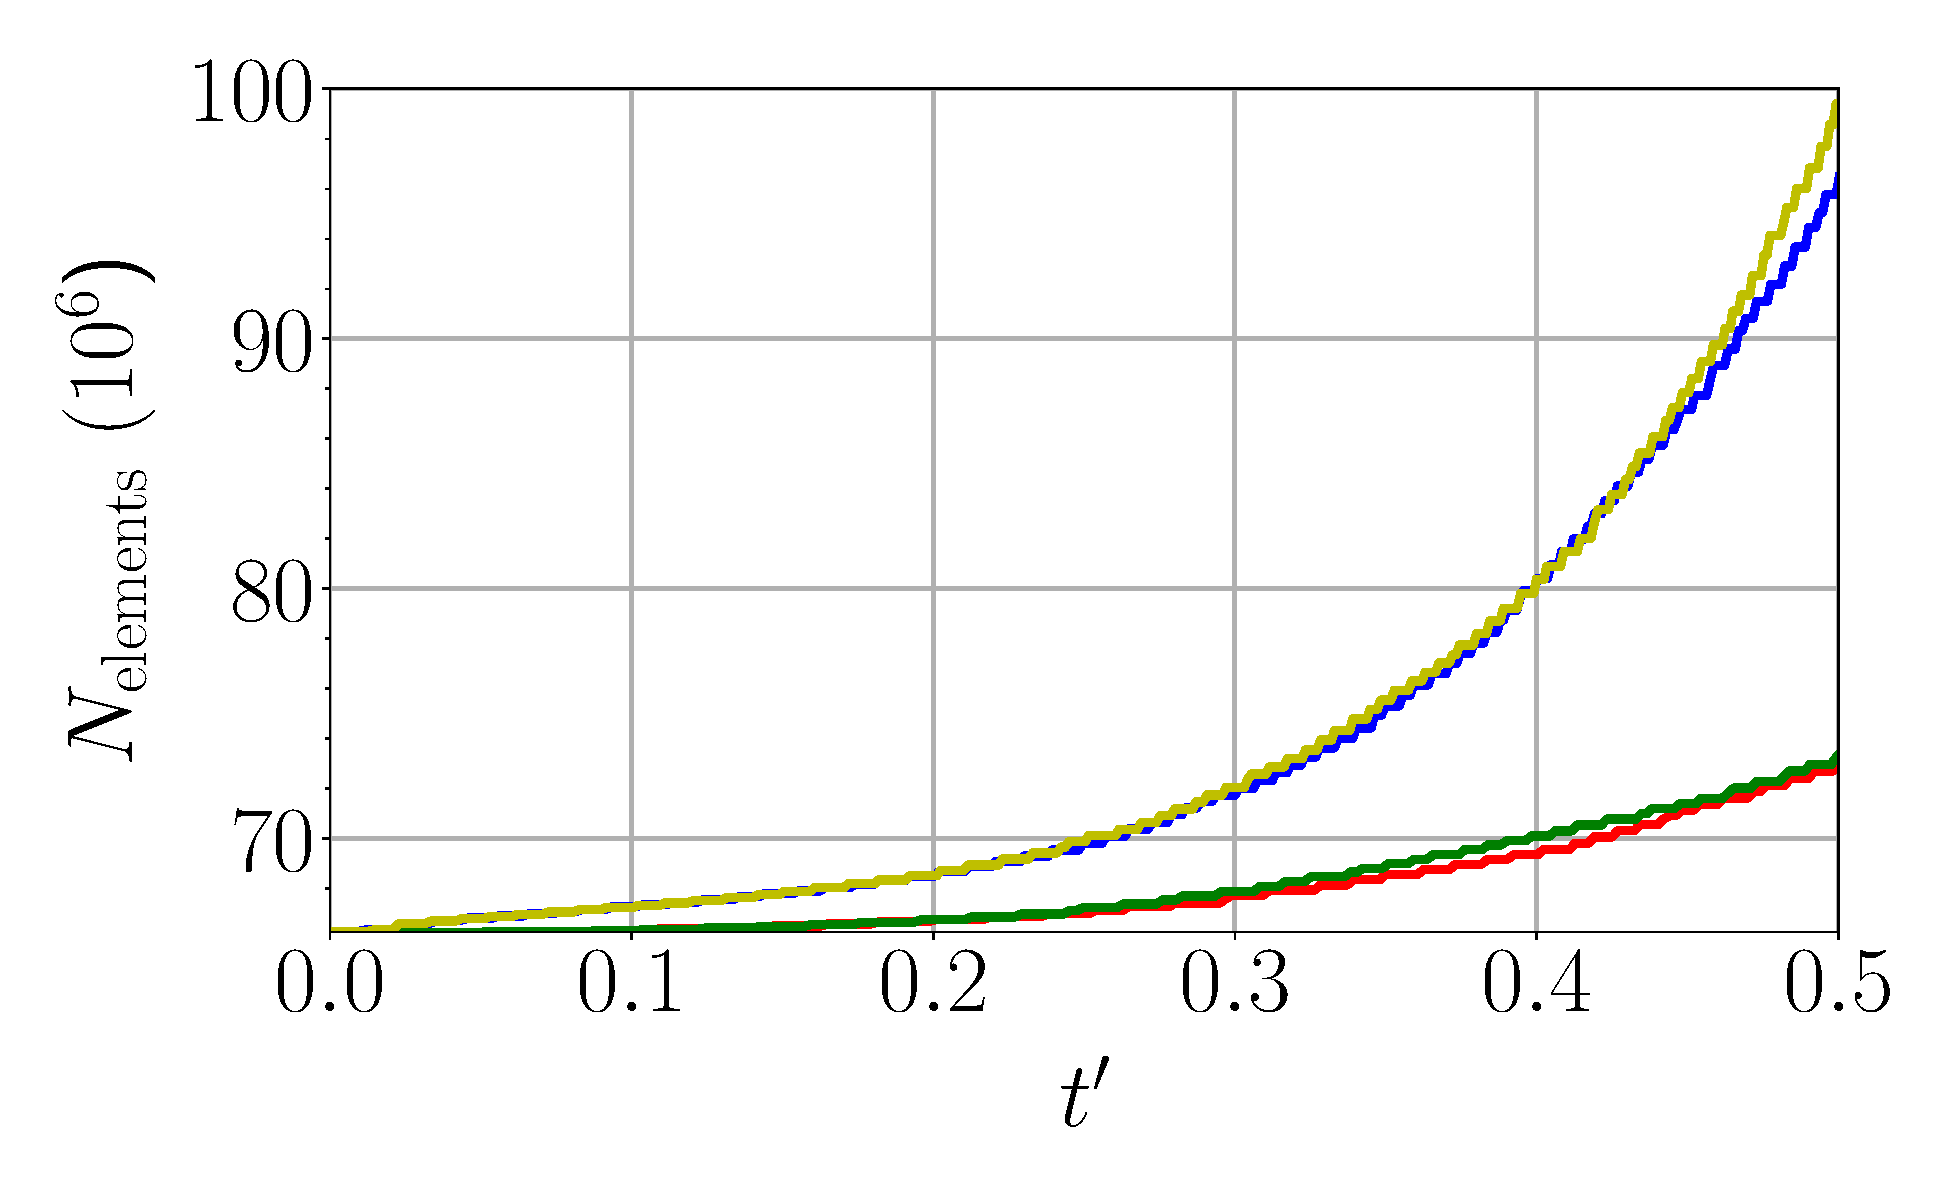
\includegraphics[scale=0.25]{./part2_developments/figures_ch5_resolved_JICF/JICF_nelem_evolution/JICF_nelem_increase_t_in_0_0p5}
   \caption{Zoomed-in view in black rectangle of Figure \ref{fig:JICF_nelem_increase_t_0_to_2}}
   \label{fig:JICF_nelem_increase_t_0_to_0p5} 
\end{subfigure}
\hfill
\begin{subfigure}[b]{0.45\textwidth}
	\centering
   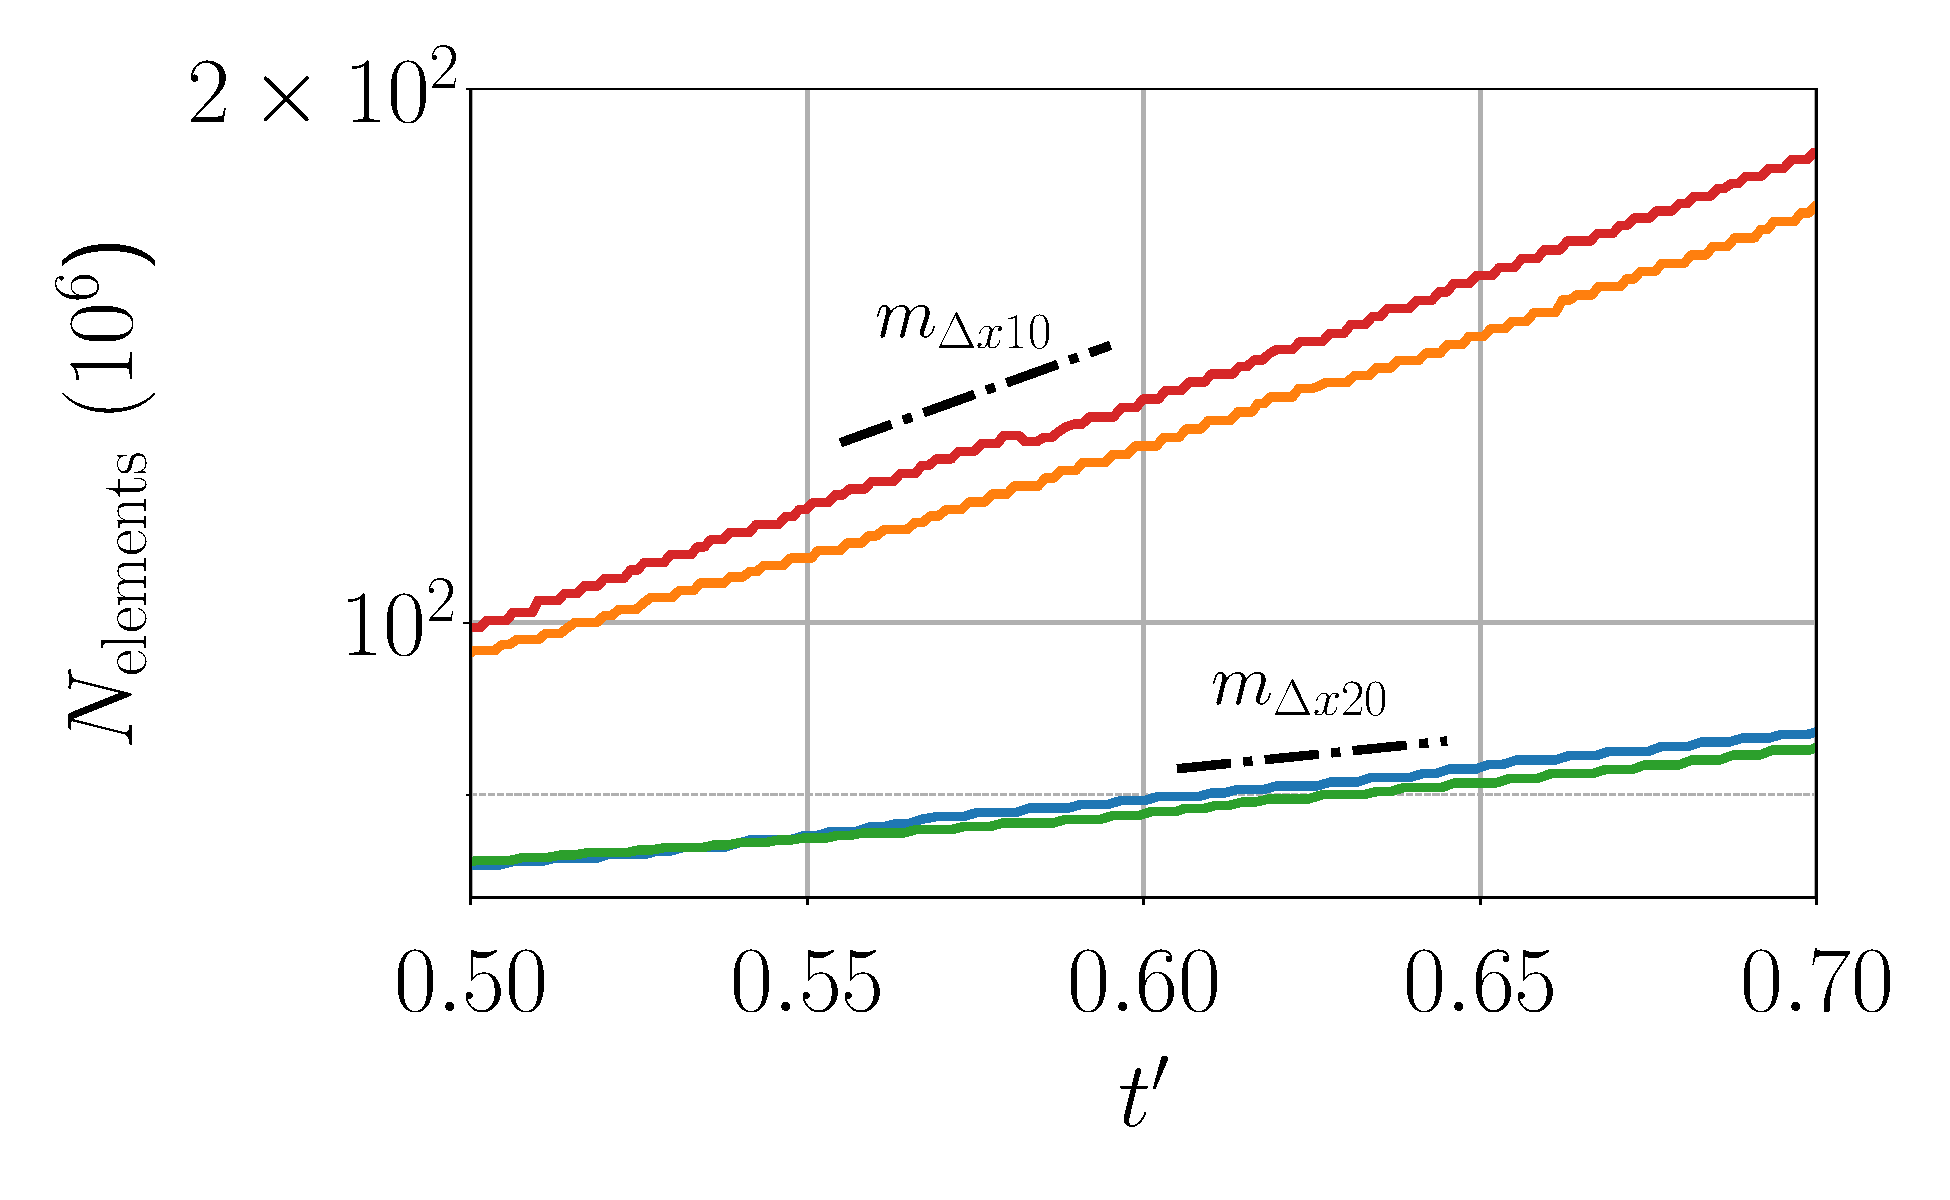
\includegraphics[scale=0.25]{./part2_developments/figures_ch5_resolved_JICF/JICF_nelem_evolution/JICF_nelem_increase_t_in_0p5_1}
   \caption{Zoomed-in view in blue rectangle of Figure \ref{fig:JICF_nelem_increase_t_0_to_2}}
   \label{fig:JICF_nelem_increase_t_0p5_to_0p7}
\end{subfigure}
   \caption{Evolution of number of mesh elements with time in JICF simulations. The dashed, black vertical line indicates the time $t^\prime = 1$ when the first droplet reaches the plane where liquid is removed.}
\label{fig:JICF_nelem_increase}
\end{figure}




\clearpage

\section{Jet trajectories}
\label{subsec:ch5_jet_trajectories_results}

Characteristics of liquid JICF were introduced in $\S$\ref{sec:ch1_fuel_injection_technology}. Among its features, the trajectory of the jet is found to be one of the most studied ones. JICF trajectoy is of paramount importance since it provides the vertical penetration of the jet and, therefore, the areas downstream injection that could possibly have presence of fuel. Design of systems involving JICF configurations often take into account the penetration, estimated either from experiments or simulations, as a relevant parameter for combustor sizing.

Jet trajectories are usually obtained for the windward side of the jet, since this is the side indicating the furthest vertical location ($z$) containing liquid for each axial location in crossflow direction ($x$). Experimental studies on JICF configurations often provide correlations for the mean trajectory relating $z$ with $x$. Some examples of correlations were given in Table \ref{tab:correlations_experimental_JICF}. Optical accesibility to the windward side of the jet by using, for example, quartz walls and visualization equipment such as high-speed cameras, makes the jet trajectory an easily accessible characteristic from the experimental point of view. Correlations are often specified for a given range of operating conditions and valid up to a certain axial location downstream the injection point, since further away the presence of droplets resulting from atomization make optical visualization more difficult.

In this work, the jet trajectories are determined for all the simulations performed. The configuration of \citeColor[becker_breakup_2002] provides the following experimental correlation, which will be used for simulations validation:

\begin{equation}
1.57 \mathrm{q}^{0.36} \ln \left( 1 + 3.81 \frac{x}{d_\mathrm{inj}} \right)
\end{equation}

which is valid for $1 < q < 12$, $90 < We_\mathrm{ae} < 2120$ and $x/d_\mathrm{inj} < 22$. The values for $d_\mathrm{inj}$ and $q$ are given
in Table \ref{tab:jicf_operating_conditions}. The authors also present a standard deviation for the correlation of $\sigma = 0.81$. By plotting this expression together with the trajectories obtained from the simulations, one has a qualitative view of the difference between simulations and experiments. To go further in the analyses, it is aimed to provide a quantitative measure of the differences between the correlation and the experimental results presented hereafter. For this purpose, an error defined as a $L_2$ norm is defined as follows:

\begin{equation}
\label{eq:L2_JICF}
    L_2 = \sqrt{\frac{1}{N}   \sum_{i=1}^N \left( \frac{z}{d_\mathrm{inj}} \Bigr|_{\mathrm{num},i} -   \frac{z}{d_\mathrm{inj}} \Bigr|_{\mathrm{exp},i} \right)^2}
\end{equation}

where $N$ is the number of points along the abscissa $x$ in which the difference between curves is evaluated and i refers to the $i$-th point. The subscript num$,i$ indicates the mean value obtained from simulations for the vertical location at point $i$, while exp$,i$ indicates the equivalent measure from experiments. From this definition it follows that the $L_2$ error is a measure of the accuracy of the simulations: the lower the $L_2$, the closer the simulation results are to experimental ones. The $L_2$ error can also be monitored with time to determine the convergence evolution of the trajectories.

Apart from the $L_2$ error, another measure for experimental accuracy can be defined as an error along the trajectory:



\begin{equation}
\label{eq:error_along_trajectory}
\varepsilon_i  =  \frac{ z/d_\mathrm{inj} \Bigr|_{\mathrm{num},i} - z/d_\mathrm{inj} \Bigr|_{\mathrm{exp},i} }{ z/d_\mathrm{inj} \Bigr|_{\mathrm{exp},i} }
\end{equation}

The error $\varepsilon_i$ is then obtained and plotted for all the abscissa values $x_i$, providing an indicator of the trajectory’s accuracy along the crossflow’s axial direction. \\

%Different methods to obtain trajectories from resolved simulations were proposed in $\S$\ref{sec:ch5_tools_jicf_trajectories}. These methods are summarized in Table \ref{tab:jicf_tools_trajectories_obtention}. In this section, firstly  the four methods described are applied to the simulation UG100\_DX20, the trajectories obtained are then compared and discussed. Secondly, the method MEAN\_GRAD is chosen to perform experimental validation with all simulations from Table \ref{tab:jicf_resolved_simulations_performed}. \hl{Finally, a comparison of the $L_2$ errors based on the maximum distance downstream in the trajectory ...}

The jet establishment discussed in $\S$\ref{subsec:ch5_JICF_flow_establishment} shows that the jet is not developed at the early instants of injection. At these stages, the quantity of liquid inside the domain is low and the gaseous field at the vicinity of the injector is not perturbed by the jet along the region where instabilities are developed and the jet starts to atomize. Hence, the jet penetration at the early instants might not be representative of the trajectory followed afterwards, and so trajectories are obtained after a certain establishment time which here is taken as 1 time of the characteristic liquid time $\tau_{\mathrm{dr}_{x=10}}$. All gaseous and liquid fields statistics (velocity, pressure, $\psi$, etc. mean and RMS values) are reinitialised after this establishment time, hence the trajectories based on the mean $\psi$ field do not consider this prompt transient. Instantaneous trajectories averaged for obtaining mean trajectories based on them are also taken after this time.

\clearpage


\subsection{Comparison of methods}

Four methods to obtain trajectories from resolved simulations were proposed in $\S$\ref{sec:ch5_tools_jicf_trajectories}. These methods are summarized in Table \ref{tab:jicf_tools_trajectories_obtention}. The trajectories obtained with each method for the case UG100\_DX20 are shown in Figure \ref{fig:JICF_trajectories_and_L2_comparison}a. The evolution of the $L_2$ errors are displayed in Figure \ref{fig:JICF_trajectories_and_L2_comparison}b.

Trajectories show two different tendencies when using the two families of methods based on instantaneous trajectories and on the mean $\psi$ field. In the vicinity of the injector all trajectories follow the same tendency up to $x/d_\mathrm{inj} \sim 1$. At this point, mean $\psi$ trajectories keep on following the experimental correlation and mean instantaneous ones are located below. \hl{The former ones show noise due to numerical dissipation in the $\psi$ field, while the later show a smoother shape since they are obtained by interpolating instantaneous trajectories and averaging them with time}. Further downstream, instantaneous-averaged trajectories overpass the ones obtained from the mean $\psi$ ones. \hl{The different trends shown by the trajectorices from both methodologies are due to their underlying definitions: instantaneous-averaged trajectories intend only to retrieve the outer contour of the jet by sweeping the $z$ axis and identifying the points with the contour $\psi = 0.5$ at the middle plane $y = 0$, while the mean-based methods take the $\overline{\psi}$ field defined in all the domain and then obtain the trajectories at the middle plane. The $\overline{\psi}$ field is diffused as opposed to the $\psi = 0.5$ contour retrieved by the instantaneous methods, so the trajectories obtained as $\max \left( \nabla_z | \overline{\psi} | \right)$ and $\overline{\psi} = 0.01$ are located in the regions where $\overline{\psi}$ is close to $0$ (i.e. where the mean presence of liquid is low). Consequently, the trajectories generated penetrate further away than the instantaneous averaged ones in the near-injector region where the liquidis coherent, while they show a different tendency downstream when atomization has taken place and dispersed droplets are present.}


\begin{figure}[ht]
\flushleft
\begin{subfigure}[b]{0.45\textwidth}
	\centering
   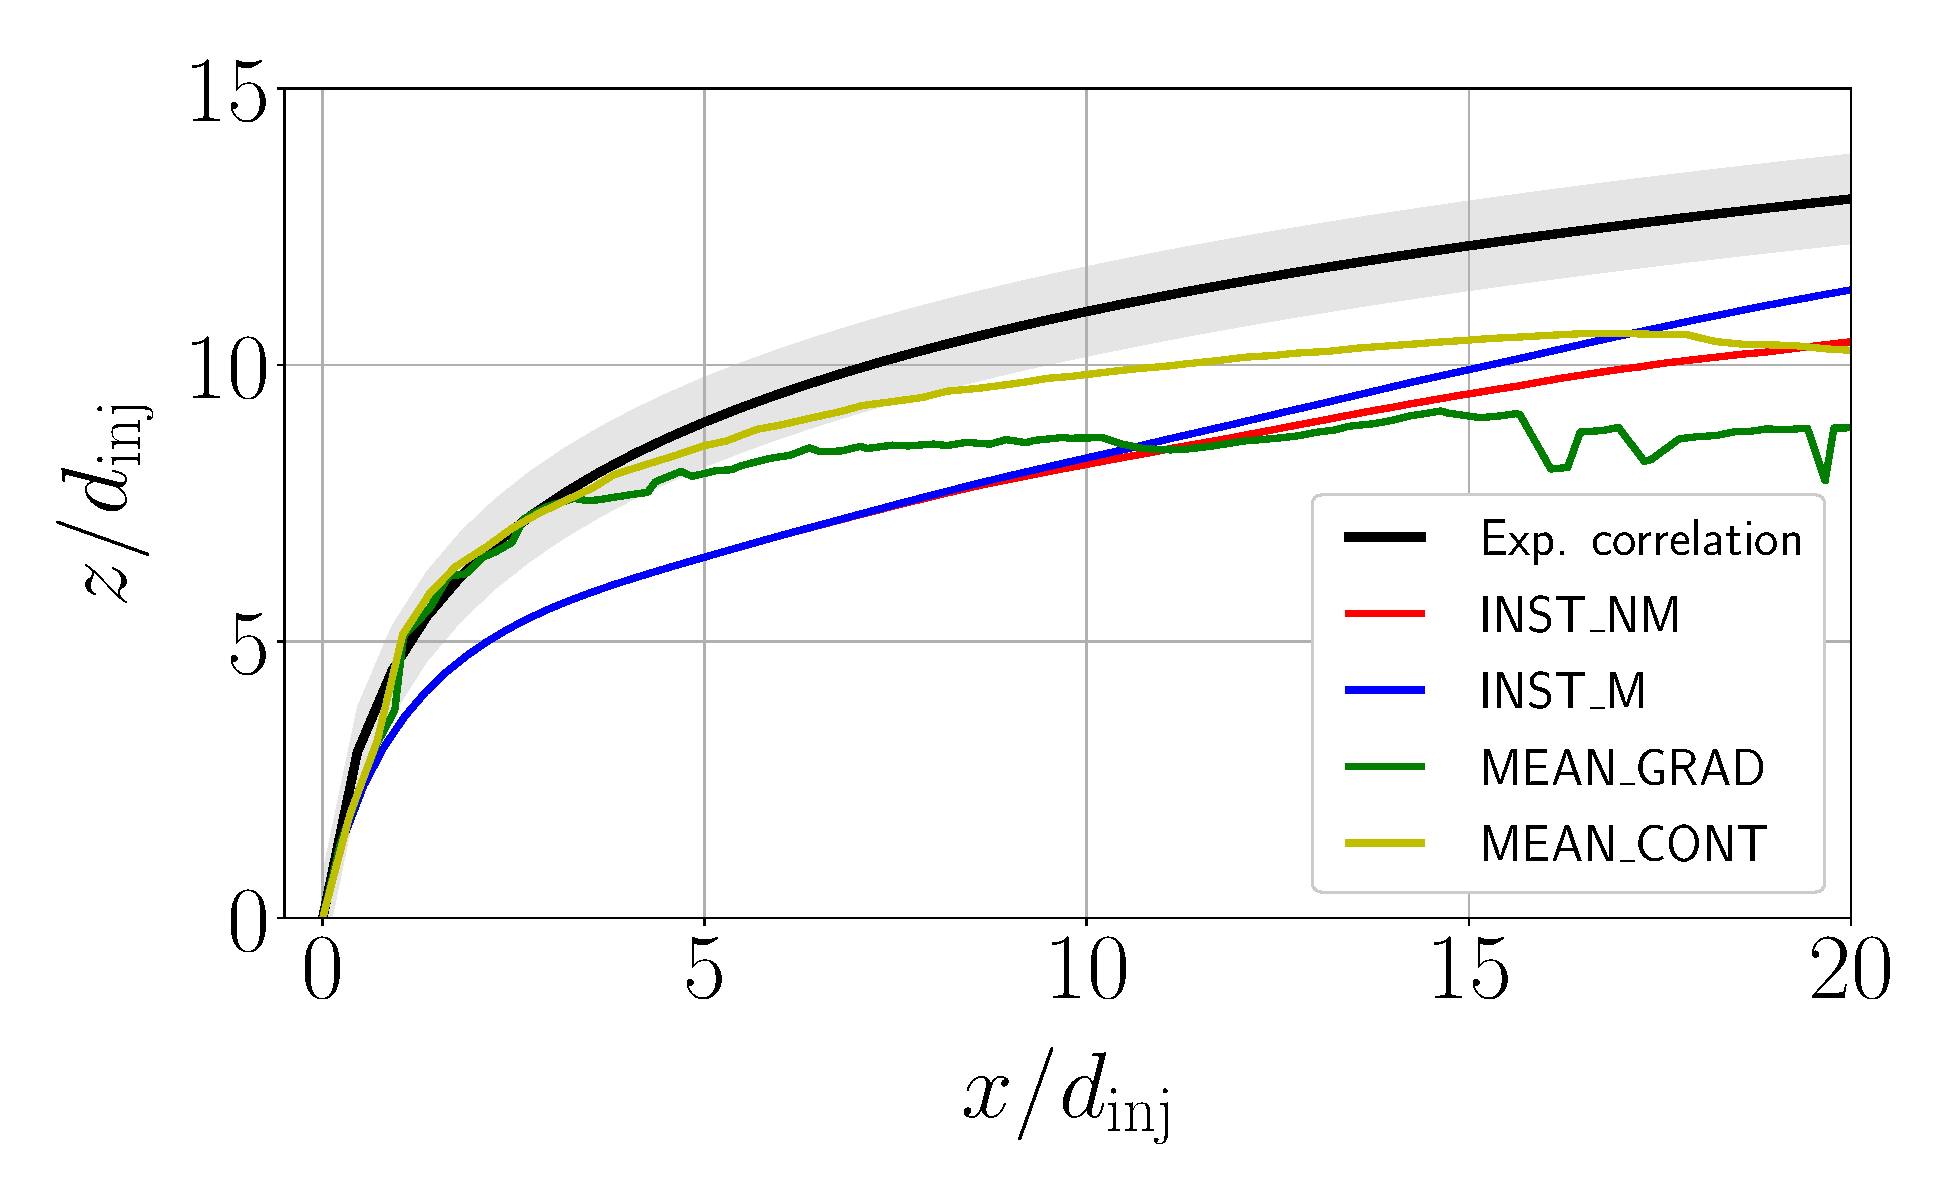
\includegraphics[scale=0.25]{./part2_developments/figures_ch5_resolved_JICF/results_trajectories/methods_comparison_trajectories_q6uG100_dx20.pdf}
   \caption{Mean trajectories}
   %\label{} 
\end{subfigure}
%\hfill
\hspace{0.25in}
\begin{subfigure}[b]{0.45\textwidth}
	\centering
   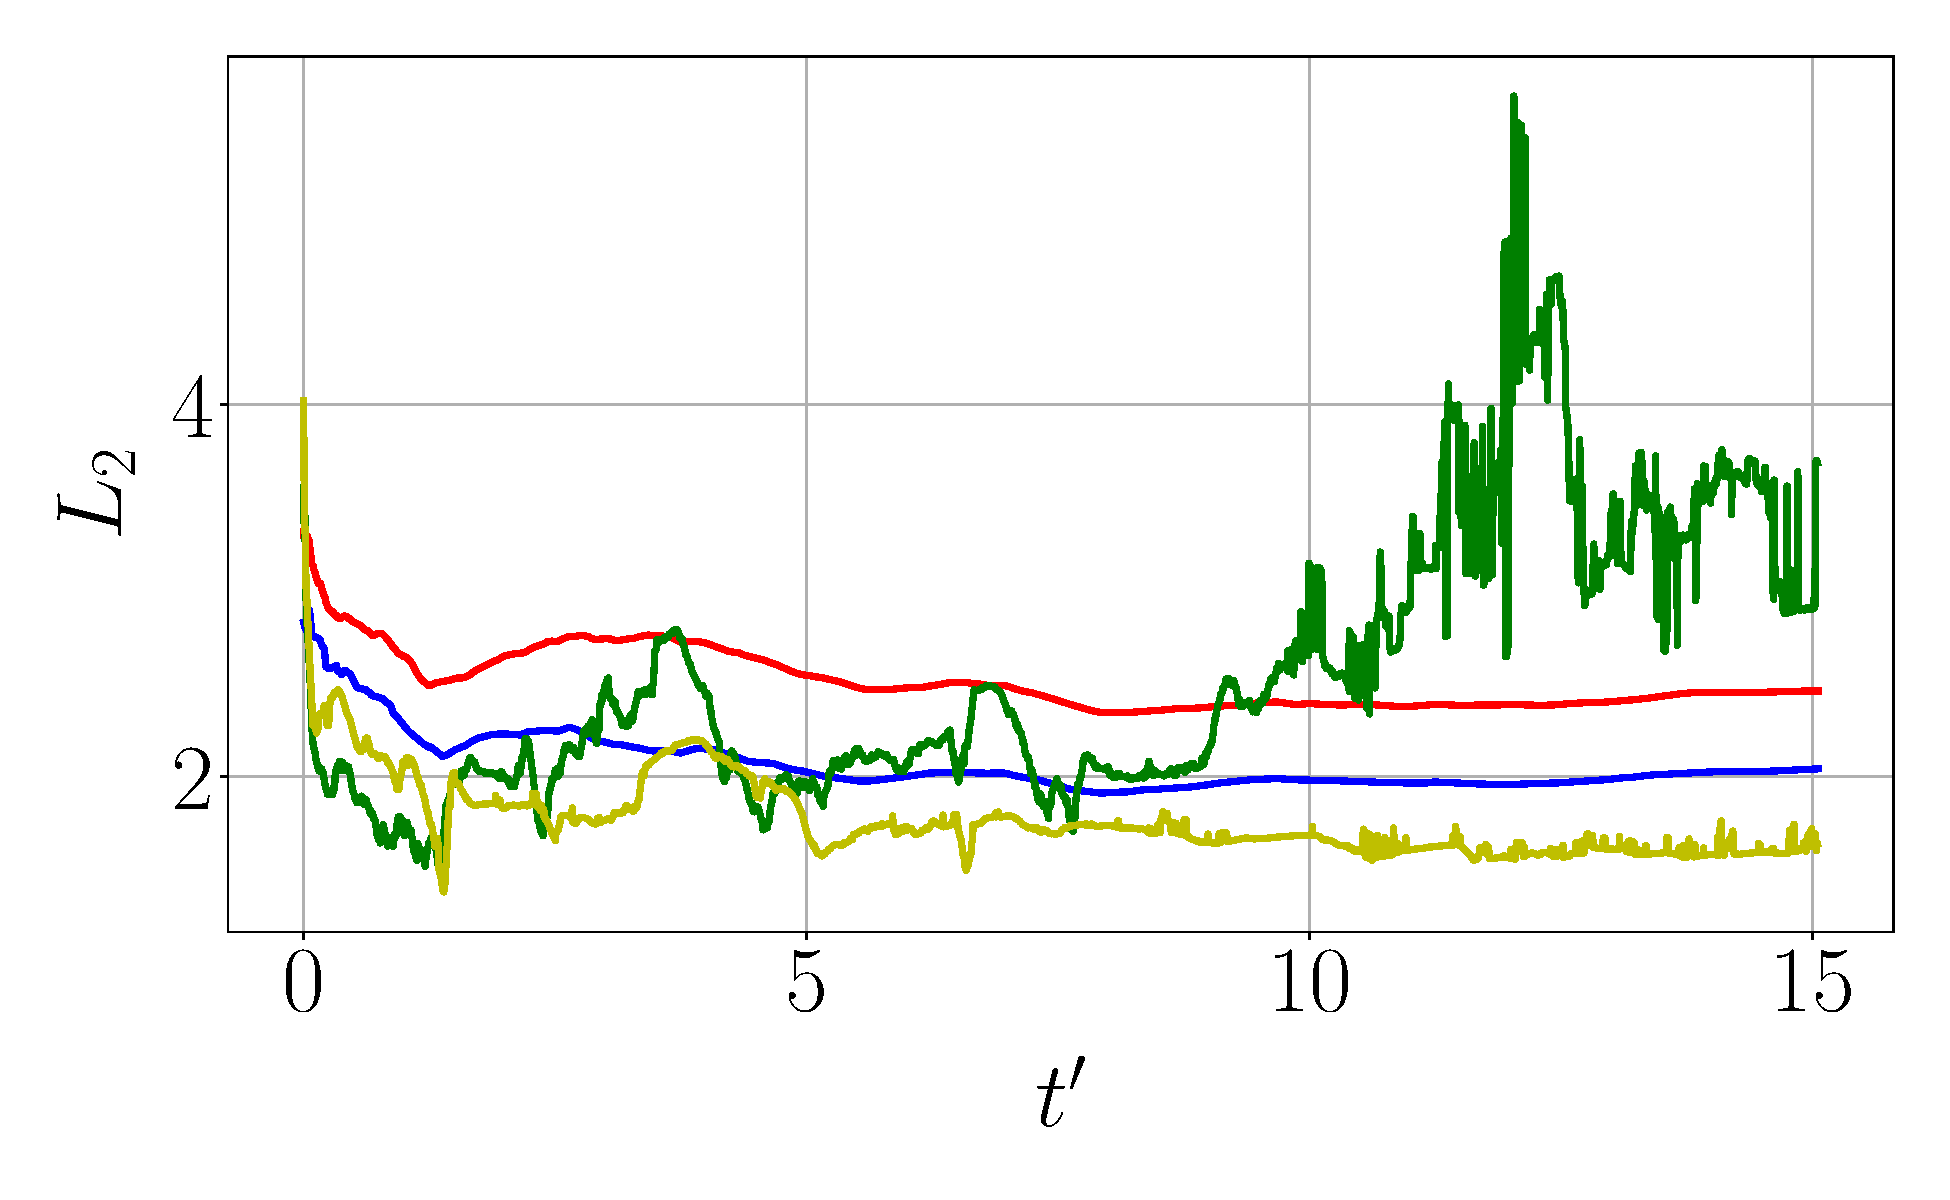
\includegraphics[scale=0.25]{./part2_developments/figures_ch5_resolved_JICF/results_trajectories/methods_comparison_L2_evolution_q6uG100_dx20.pdf}
   \caption{$L_2$ error evolution}
   %\label{}
\end{subfigure}
\caption{Trajectories and $L_2$ errors obtained with different methods for case UG100\_DX20}
\label{fig:JICF_trajectories_and_L2_comparison}
\end{figure}

\hl{Trajectories obtained from the mean $\psi$ field follow the experimental correlation up to $x/d_\mathrm{inj} \sim 4$, at which point the curve obtained with the gradient method is underestimated with respect to the iso-contour of $\overline{\psi} = 0.01$. This might indicate that at this point primary atomization starts to take place and ligaments are being stripped-off the jet \textbf{CHECK THIS WITH SOME PICTURE}. The $\overline{\psi}$ generated downstream due to the presence of firstly ligaments and then droplets makes the chosen contour $\psi = 0.01$ to be further away than the $\max \left( \nabla_z | \overline{\psi} | \right)$ one, since this low value means that the liquid presence with is scarce. Nevertheless, it must be considered that the chosen value for the iso-contour of $\overline{\psi}$ is arbitraty as explained in $\S$}\ref{sec:ch5_tools_jicf_trajectories} \hl{and the trajectory obtained further downstream is very sensitive to this value. Further research is required to find a relation between the trajectories obtained with both methods}.

Both monotonic and non-monotonic trajectories follow the same tendency up to $x/d_\mathrm{inj} \sim 10$, then they diverge. This is coherent with the definition of both methods, as the monotonic one neglects liquid structures detected which not follow an increasing trend with $x$ and non-monotonic ones do consider those, as explained in Figures \ref{fig:trajectory_obtention_instantaneous_method_a} and \ref{fig:trajectory_obtention_instantaneous_method_b}. In effect, for $x/d_\mathrm{inj} > 10$ primary atomization has already taken place and a polydisperse spray composed of many droplets is found (dispersed phase). Some droplets found in this region when sweeping along the $z$ axis to detect liquid structures do not belong to the outer trajectory of the jet. Since these droplets are neglected in the monotonic method but considered in the non-monotonic one, the averaging procedure of all interpolated, instantaneous trajectories produces a further penetrating curve for the monotonic procedure than for the non-monotonic one.

The evolution of the $L_2$ norm for all four methods is shown in Figure \ref{fig:JICF_trajectories_and_L2_comparison}b. Establishment of the curves is observed in all cases for $t^{\prime} > 5$ (\textbf{OJO: comprobar norma L2 de metodo MEAN\_GRAD !!!}). This indicates that the trajectories are overall converged at this stage. More fluctuations are observed in the $\overline{\psi}$ methods than in the instantaneous-averaged ones. The monotonic and non-monotonic curves show a smooth development with time, and both follow the same tendency except for a threshold in the $L_2$ norm caused by the downstream difference in the trajectories at Figure \ref{fig:JICF_trajectories_and_L2_comparison}a. The lowest error is obtained with the $\overline{\psi} = 0.01$ contour.


\subsection{Experimental validation}

For validating the trajectories in all simulations from Table \ref{tab:jicf_resolved_simulations_performed}, the method MEAN\_GRAD is retrieved due to its similary with the methodology followed by \citeColor[becker_breakup_2002] to obtain the experimental correlation. Results are shown in Figure \ref{fig:JICF_trajectories_validation} for both operating points, including the case for the high $We$ number without synthetic turbulence injection.

The trajectories from Figures \ref{fig:JICF_trajectories_validation}a and b show a high dependence on the interface mesh resolution $\Delta x_\mathrm{min}$ for both operating points. Both resolutions coincide with the experimental correlation up to $x/d_\mathrm{inj} \sim 5$ for low $We$ and to $x/d_\mathrm{inj} \sim 4$ for high $We$. Further upstream, the coarse resolution $\Delta x_\mathrm{min} = 20~\mu m$ is underestimated with respect to experiments, while the fine one $\Delta x_\mathrm{min} = 10~\mu m$ continues following the correlation until it surpasses it. The difference with interface resolution is due to the presence of instabilities in the windward side of the jet, which are obtained for the fine cell size but not for the coarse one as observed in Figures \ref{fig:JICF_establishment_UG100_lateral} to \ref{fig:JICF_establishment_UG75_top}. \hl{The presence of instabilities in the fine simulations creates ligaments and droplets with higher inertia that penetrate further away than those generated in the coarse simulations, as explained in }$\S$\ref{subsec:ch5_instabilities_presence}. As a consequence, the resulting trajectories in the fine simulations penetrate further than both the coarse ones and the experimental correlation after atomization takes place. 

\begin{figure}[ht]
\flushleft
\begin{subfigure}[b]{0.45\textwidth}
	\centering
   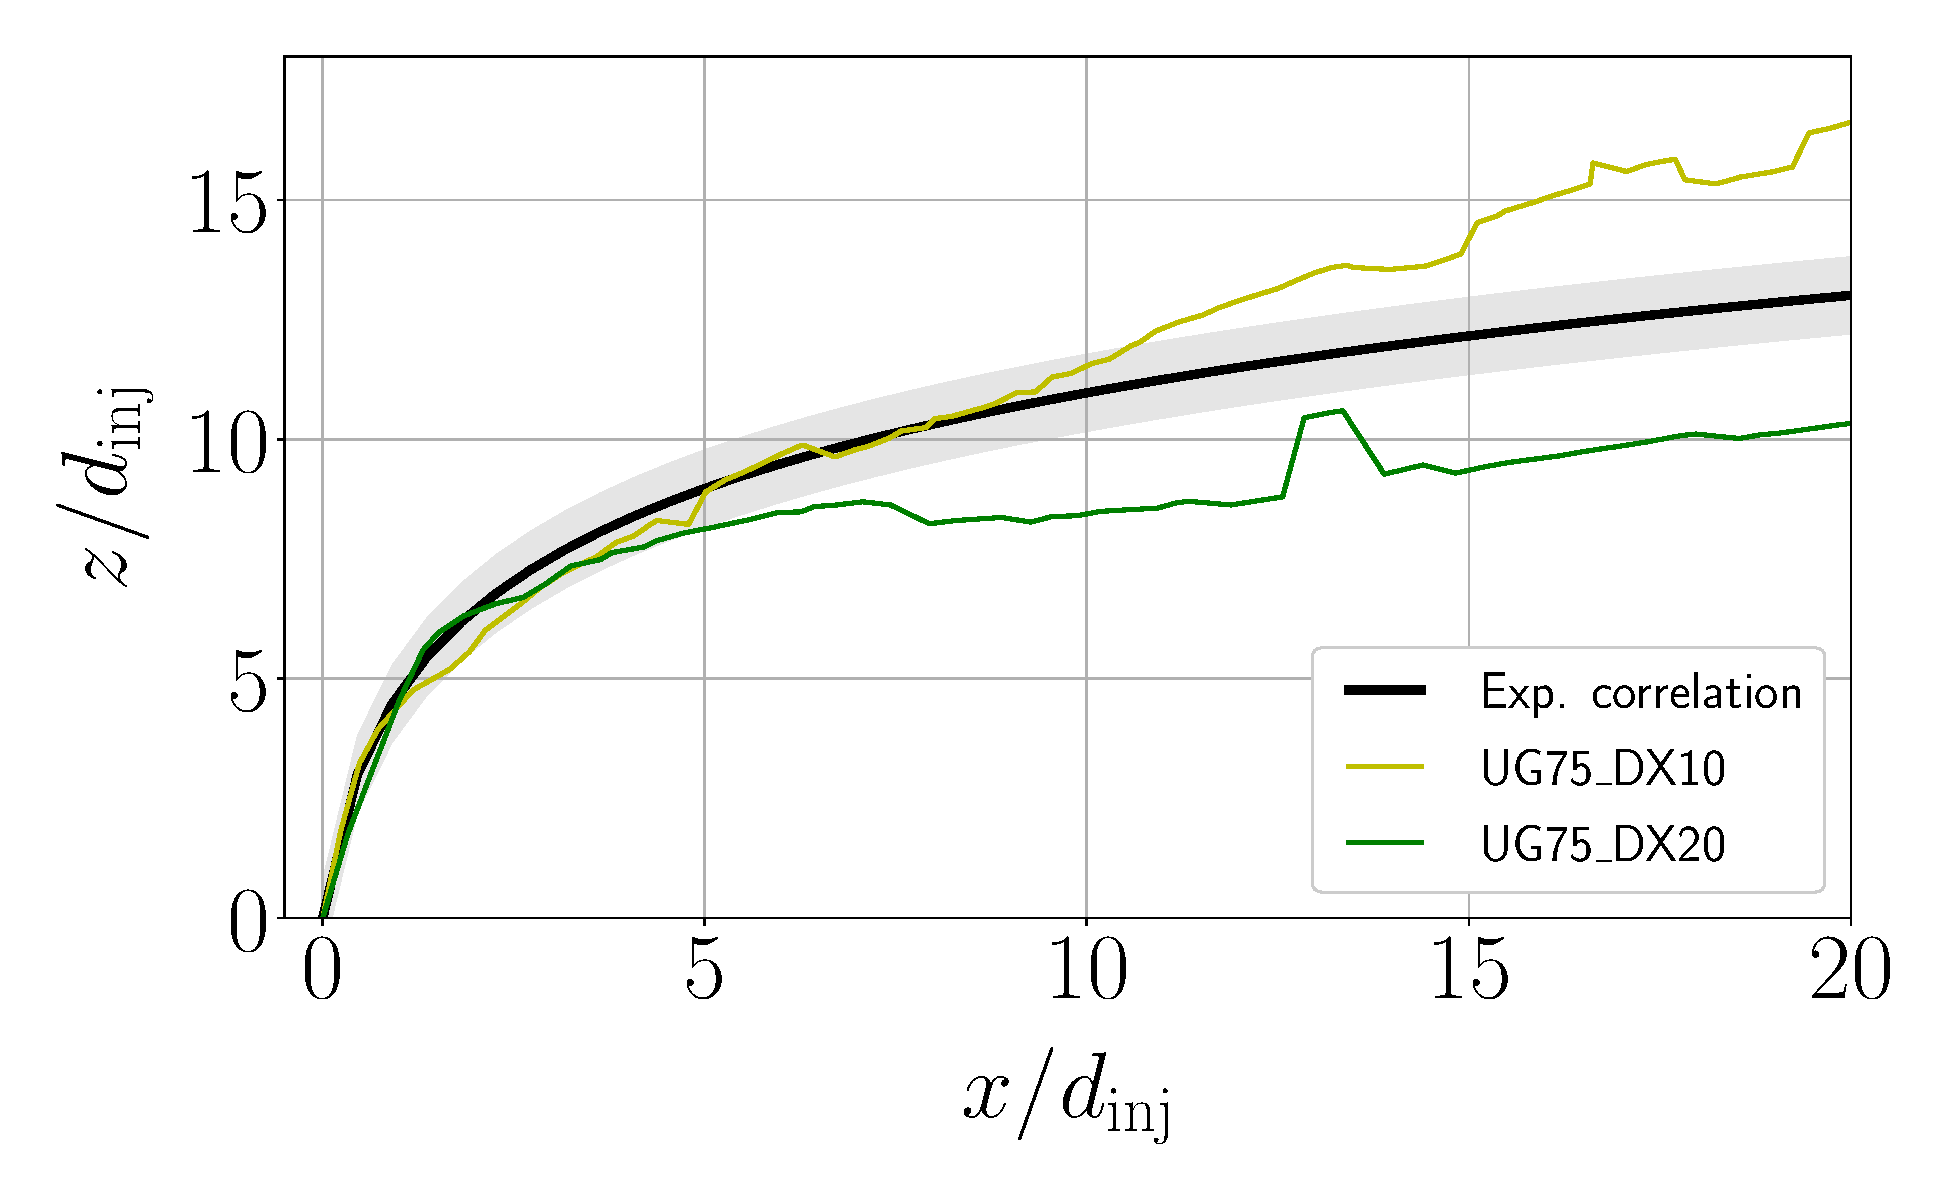
\includegraphics[scale=0.25]{./part2_developments/figures_ch5_resolved_JICF/results_trajectories/methods_expe_validation_trajectories_q6uG75.pdf}
   \caption{Low $We$ trajectories}
   %\label{} 
\end{subfigure}
%\hfill
\hspace{0.25in}
\begin{subfigure}[b]{0.45\textwidth}
	\centering
   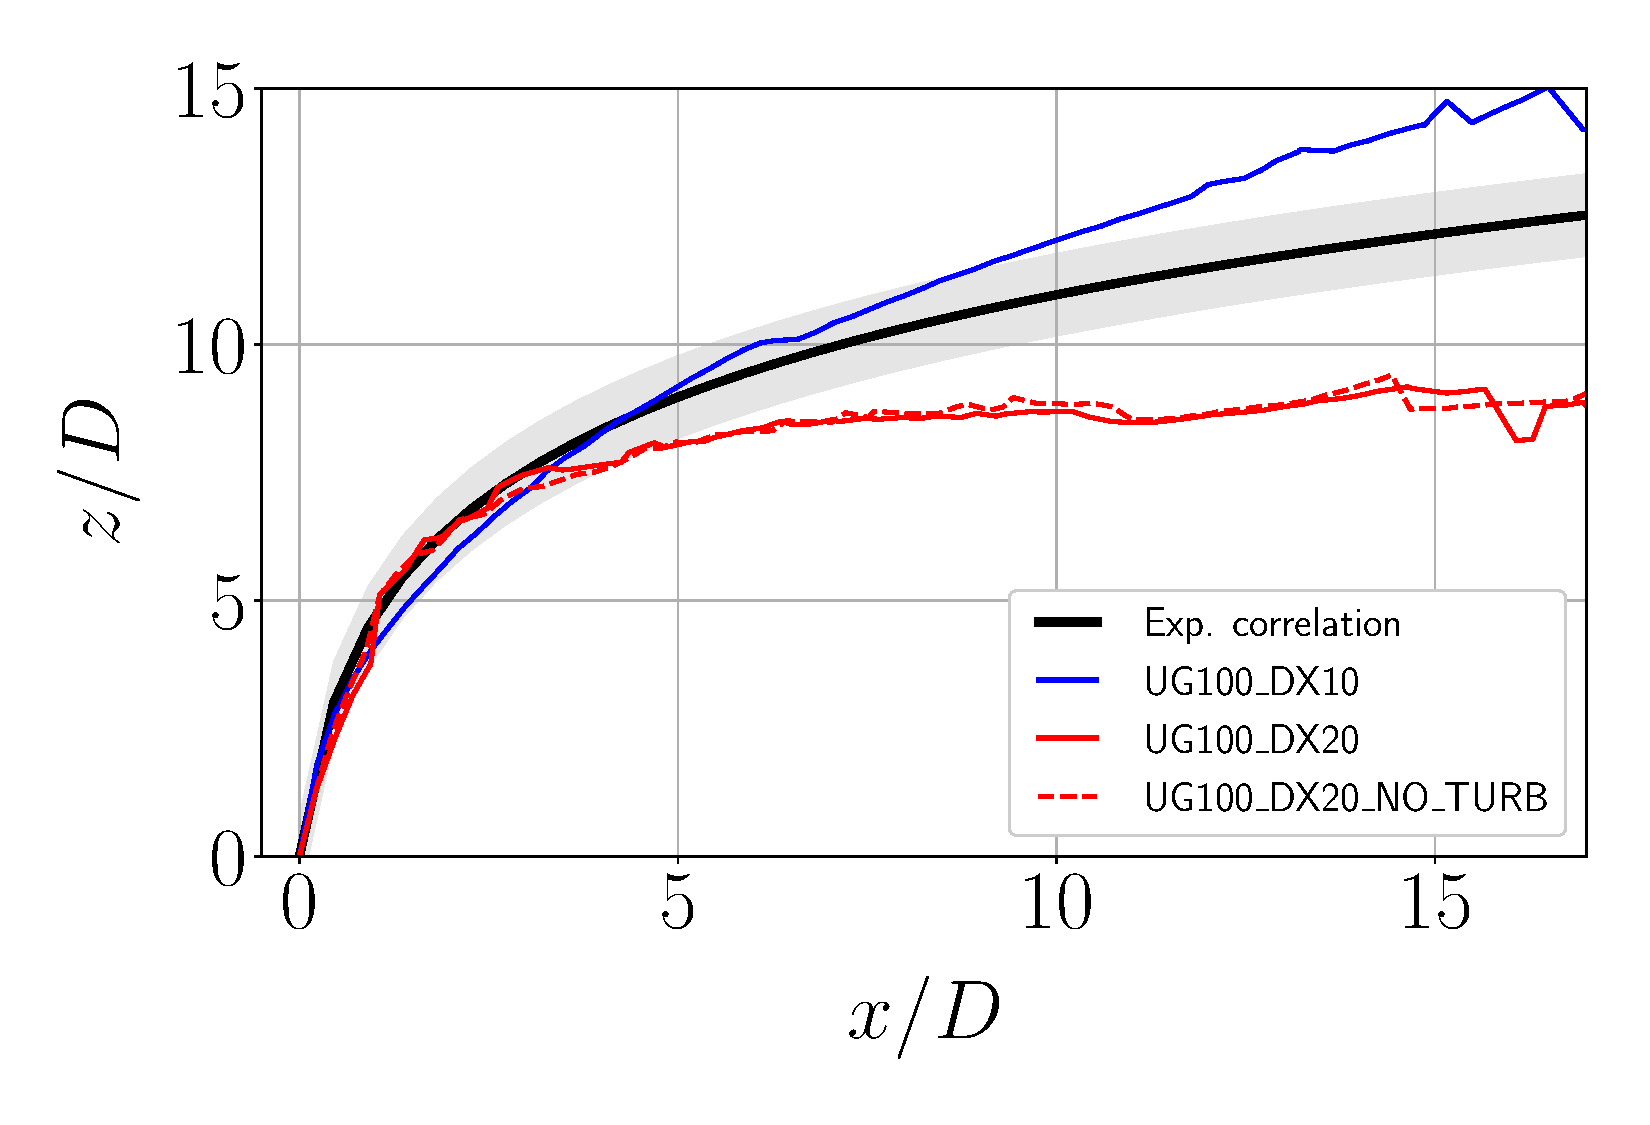
\includegraphics[scale=0.25]{./part2_developments/figures_ch5_resolved_JICF/results_trajectories/methods_expe_validation_trajectories_q6uG100.pdf}
   \caption{High $We$ trajectories}
   %\label{}
\end{subfigure}

\vskip\baselineskip

\begin{subfigure}[b]{0.45\textwidth}
	\centering
   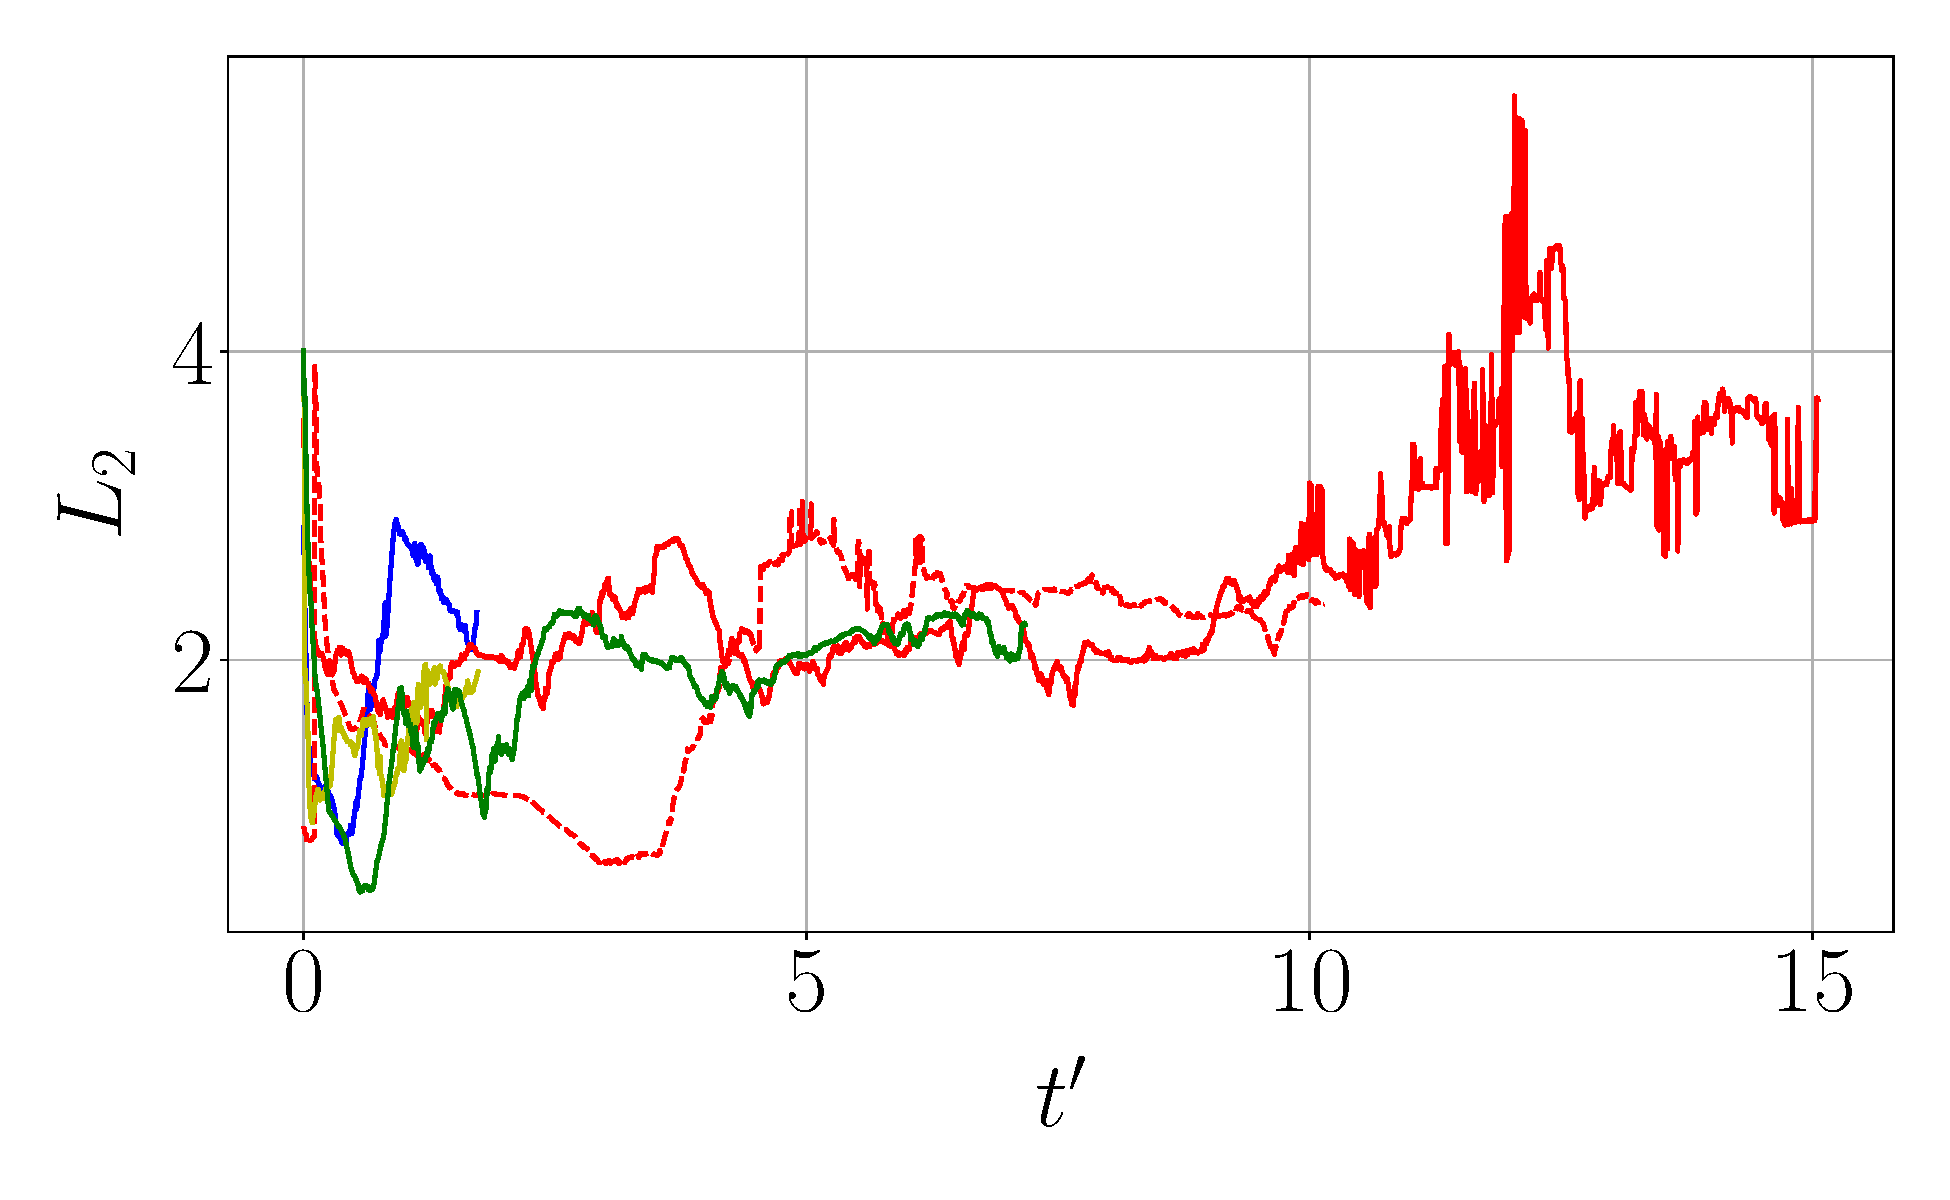
\includegraphics[scale=0.25]{./part2_developments/figures_ch5_resolved_JICF/results_trajectories/methods_expe_validation_L2_evolution.pdf}
   \caption{Evolution of $L_2$ norms with time.}
   %\label{} 
\end{subfigure}
%\hfill
\hspace{0.25in}
\begin{subfigure}[b]{0.45\textwidth}
	\centering
   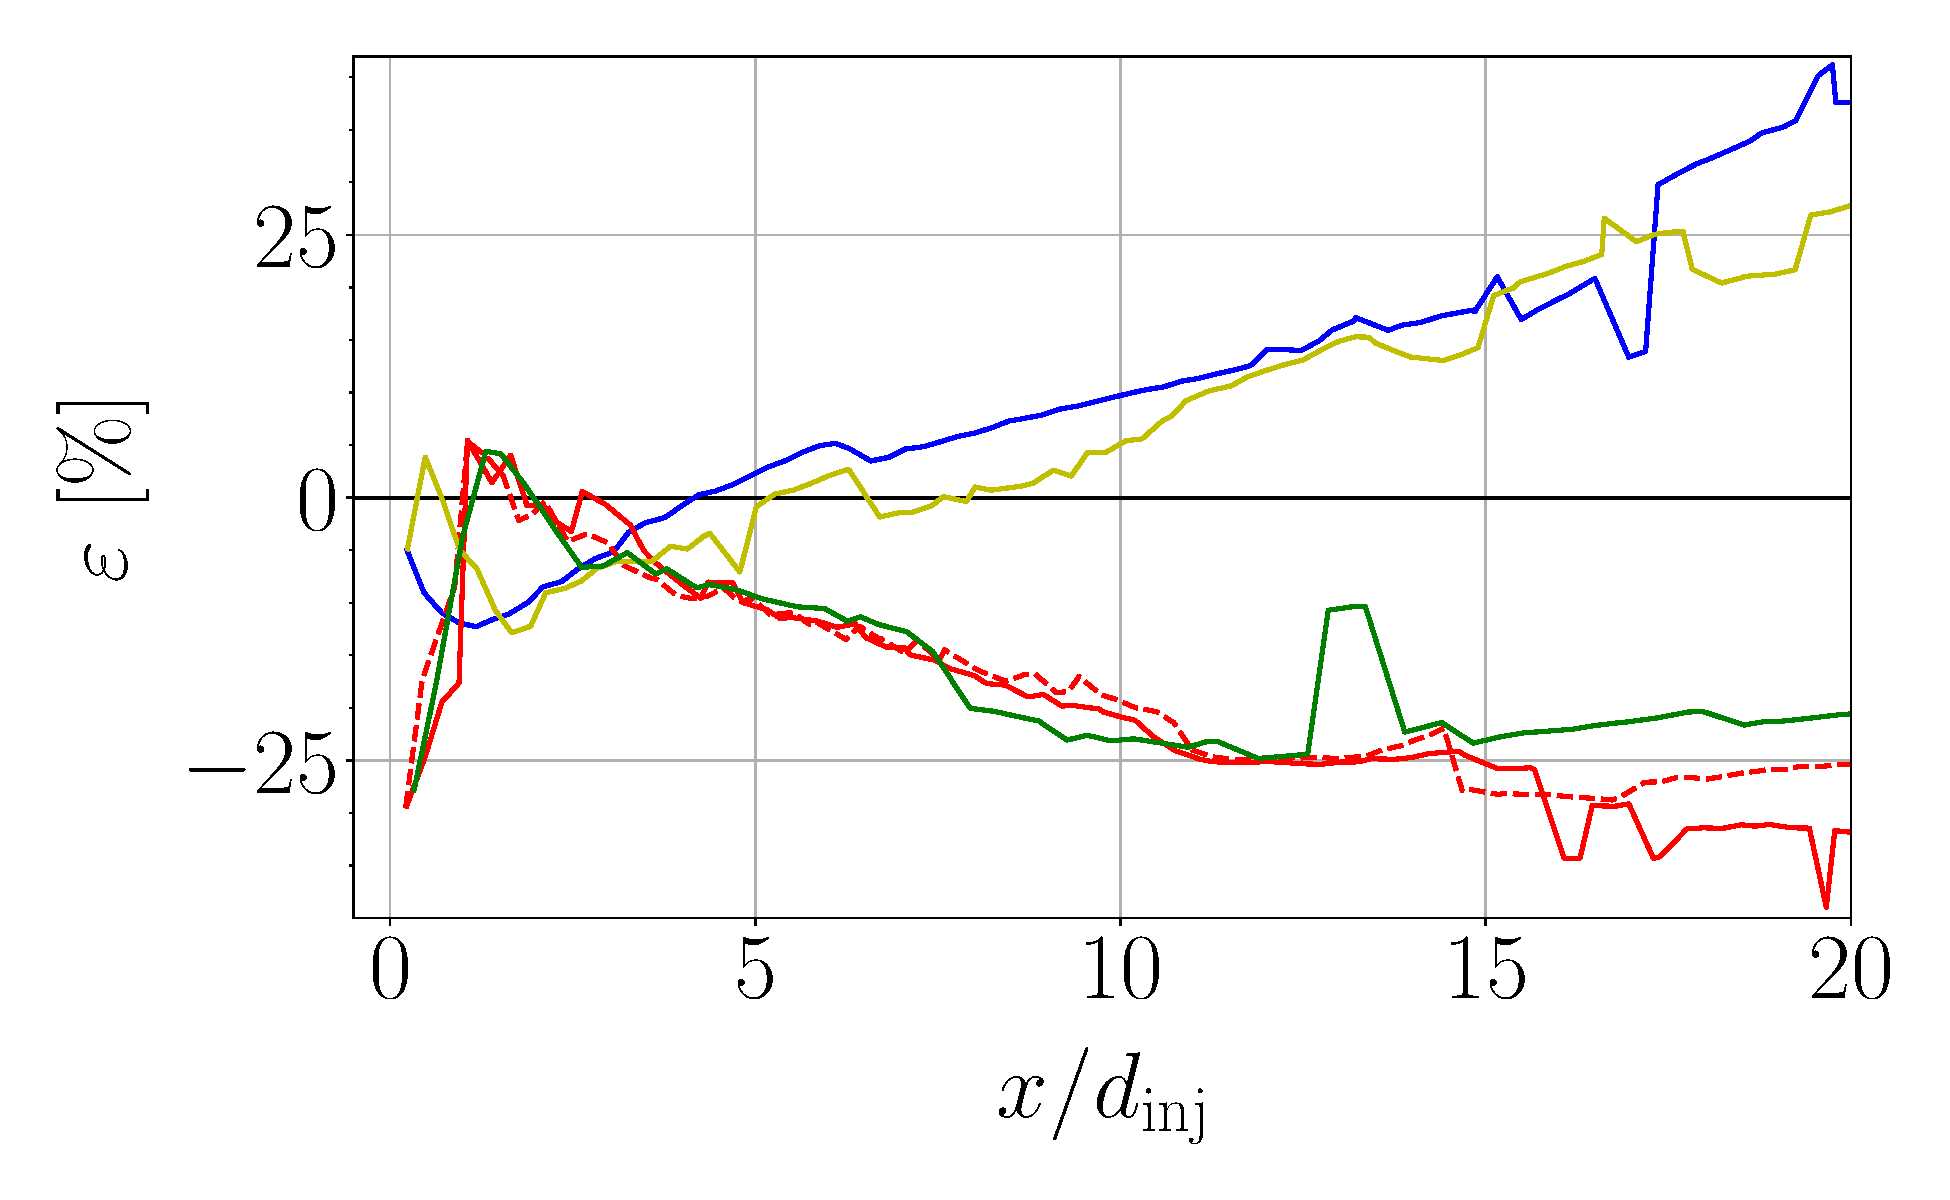
\includegraphics[scale=0.25]{./part2_developments/figures_ch5_resolved_JICF/results_trajectories/methods_expe_validation_error_with_xD.pdf}
   \caption{Error $\varepsilon$ along trajectory}
   %\label{}
\end{subfigure}

\caption{Trajectories and errors obtained with method MEAN\_GRAD}
\label{fig:JICF_trajectories_validation}
\end{figure}

\clearpage




Regarding the effect of injecting turbulence at the gaseous inlet, the red lines of Figure \ref{fig:JICF_trajectories_validation}b show that the mean trajectory is not affected when turbulence is added. \hl{This indicates that ...}

Figure \ref{fig:JICF_trajectories_validation}c shows the $L_2$ norm evolution. \hl{All cases show high fluctuations at the beginning and then stabilization towards a value of 2. The coarse simulations have been run further than the fine ...}

\begin{table}[!h]
\centering
\caption{$L_2$ errors for JICF simulations performed.}
\begin{tabular}{cc}
\thickhline
Case &  $L_2$ \\
\thickhline 
UG75\_DX10 & ? \\
UG75\_DX20 & ?  \\
UG100\_DX10 & ? \\
UG100\_DX20 & ?  \\
UG100\_DX20\_NO\_TURB & ? \\
\thickhline
\end{tabular}
\label{tab:jicf_L2_errors}
\end{table}



Finally, the relative error along the trajectory $\varepsilon$ is displayed in Figure \ref{fig:JICF_trajectories_validation}c. Negative values indicate underestimation with respect to the experimental correlation, while positive valies indicate overestimation. Close to the injection point the errors for the coarse resolutions are large since the denominator of Eq. (\ref{eq:error_along_trajectory}) is small, so short differences produce high relative errors. \hl{Then, errors }

We can also define a slip velocity:

\begin{equation}
\overline{\textbf{u}}_{\mathrm{sl}} = \overline{\textbf{u}}_l - \overline{\textbf{u}}_g
\end{equation}

\clearpage

\section{Dense core characterization}
\label{subsec:ch5_dense_core_in_ACLS_simus}



Resolved simulations are characterized by the presence of the liquid dense core, which perturbs the incoming air and creates turbulence downstream the injector. To illustrate this disturbance, the instantaneous axial fluctuations $u'$ and the jet interface are plotted in the middle plane y = 0 in Figure \ref{fig:results_dense_core_modeling_up_field} left. The dense core creates turbulence downstream the injection point, as shown by the high fluctuations in velocity. Such perturbations can have a great impact on spray dispersion once atomization has taken place, therefore modelling this perturbance effect as accurate as possible is paramount for performing dispersed-phase simulations presented in Chapter \ref{ch6:jicf_lgs_simulations}, where the dense core is neglected and a developed spray is injected.

\begin{figure}[ht]
\centering
\includeinkscape[inkscapelatex=false,scale=0.75]{./part2_developments/figures_ch5_resolved_JICF/results_dense_core_modeling/up_field_instantaneous}
\caption[Perturbation effect of the liquid dense core in the gaseous field.]{Instantaneous $u'$ field in a JICF simulation from case UG100\_DX20. The black contours indicate the lines with zero instantaneous fluctuation $u' = 0$, while the white contours denote the location of the interface at the plane.}
\label{fig:results_dense_core_modeling_up_field}
\end{figure}

In this section, the estimation of the break point and the pressure difference from the resolved simulations are presented. These are useful to define an actuator for the dispersed phase simulations according to the model introduced in $\S$\ref{sec:ch4_dense_core_modelling}. Then, the turbulent gaseous structures created by the dense core are analyzed, which are compared in Chapter \ref{ch6:jicf_lgs_simulations} with the turbulent structures created by the imposed actuator in the dispersed-phase simulations \hl{to give an idea on the accuracy of the actuator model developed in this work}. \hl{Finally, a spectral study is performed to give an idea of the characteristic frecuencies of fluctuations created ...}


\subsection{Obtention of breakup point}

The methodology proposed to obtain the breakup point in resolved simulations was explained in $\S$\ref{subsec:ch5_jet_dense_core_extraction}. Its width $w$ and coordinates $x_\mathrm{b}, z_\mathrm{b}$ obtained in the middle plane $y = 0$ are monitored with time. 

In first place, the instantaneous evolution with time of the breakup point coordinates and width are shown in Figure \ref{fig:JICF_xb_zb_w_evolution}. \hl{The time has been non-dimensionalized according to Eq.} (\ref{eq:t_prime_with_tau_drx10}). All signals display a sawtooth shape that reflects the dynamic behaviour of the dense core: increasing parameters are due to an ligaments that start to be formed from the dense core (i.e. the breakup point $x_\mathrm{b}, z_\mathrm{b}$ moves further downstream and upper, while the width $w$ increases due to the deformation of the dense core cross-section, as shown in Figure \textbf{XX}), then they suffer an abrupt decrease when the ligaments are dettached from the jet, and the process repeats once and again. Therefore, \hl{the associated frequencies to the displayed signals are of the order of the frequencies of ligament stripping. Spectra are shown in ...}.  This periodic behaviour has been observed in several experimental studies for the breakup point coordinates $x_\mathrm{b}, z_\mathrm{b}$ \citepColor[wang_characterization_2011, prakash_liquid_2018], while no signals on the width $w$ evolution have been reported in literature to the knowledge of the authors.


\begin{figure}[ht]
\flushleft
\begin{subfigure}[b]{0.45\textwidth}
	\centering
   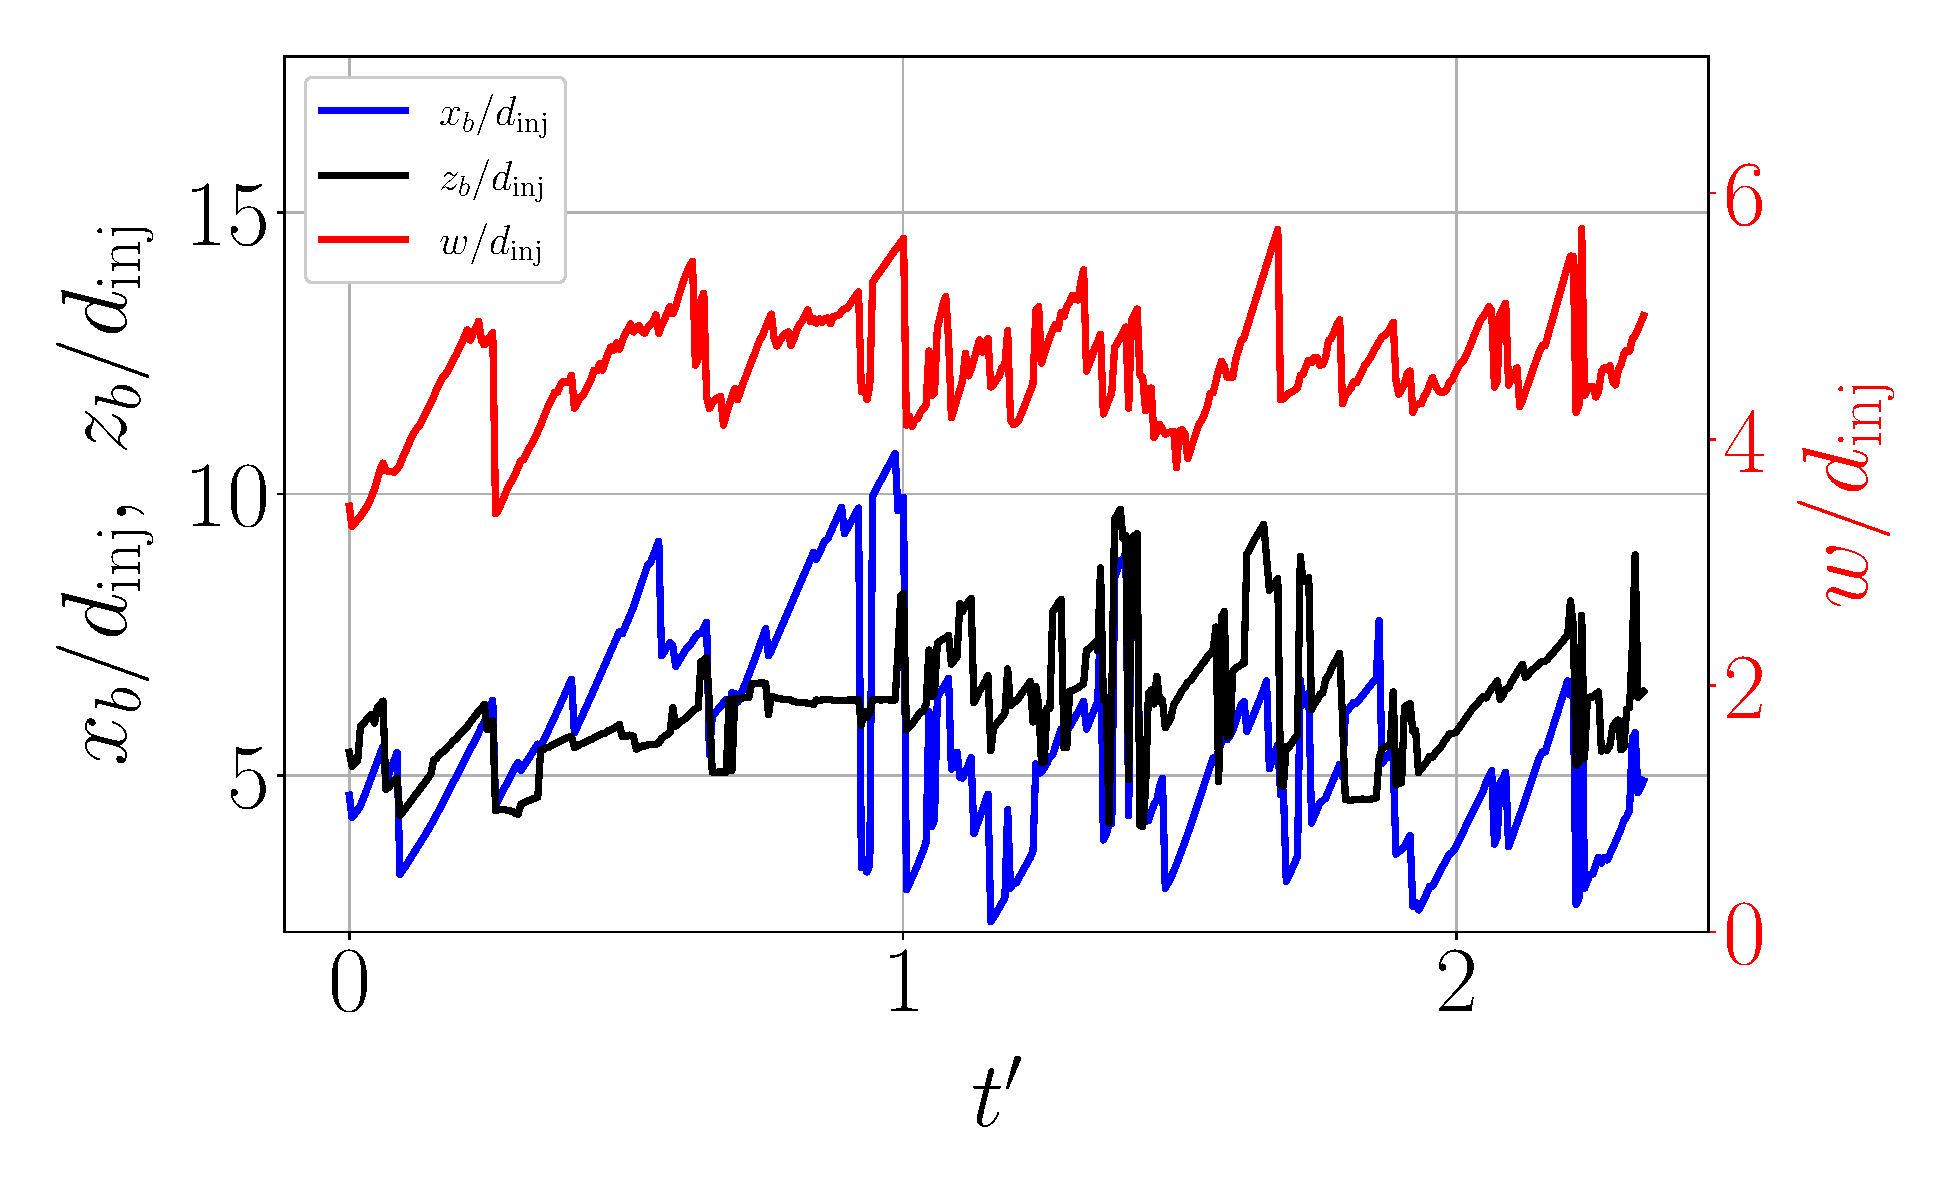
\includegraphics[scale=0.25]{./part2_developments/figures_ch5_resolved_JICF/results_dense_core_modeling/instant_xb_zb_w_UG75_DX10}
   \caption{Case UG75\_DX10}
   \label{fig:instant_xb_zb_w_UG75_DX10} 
\end{subfigure}
\hfill
\begin{subfigure}[b]{0.45\textwidth}
	\centering
   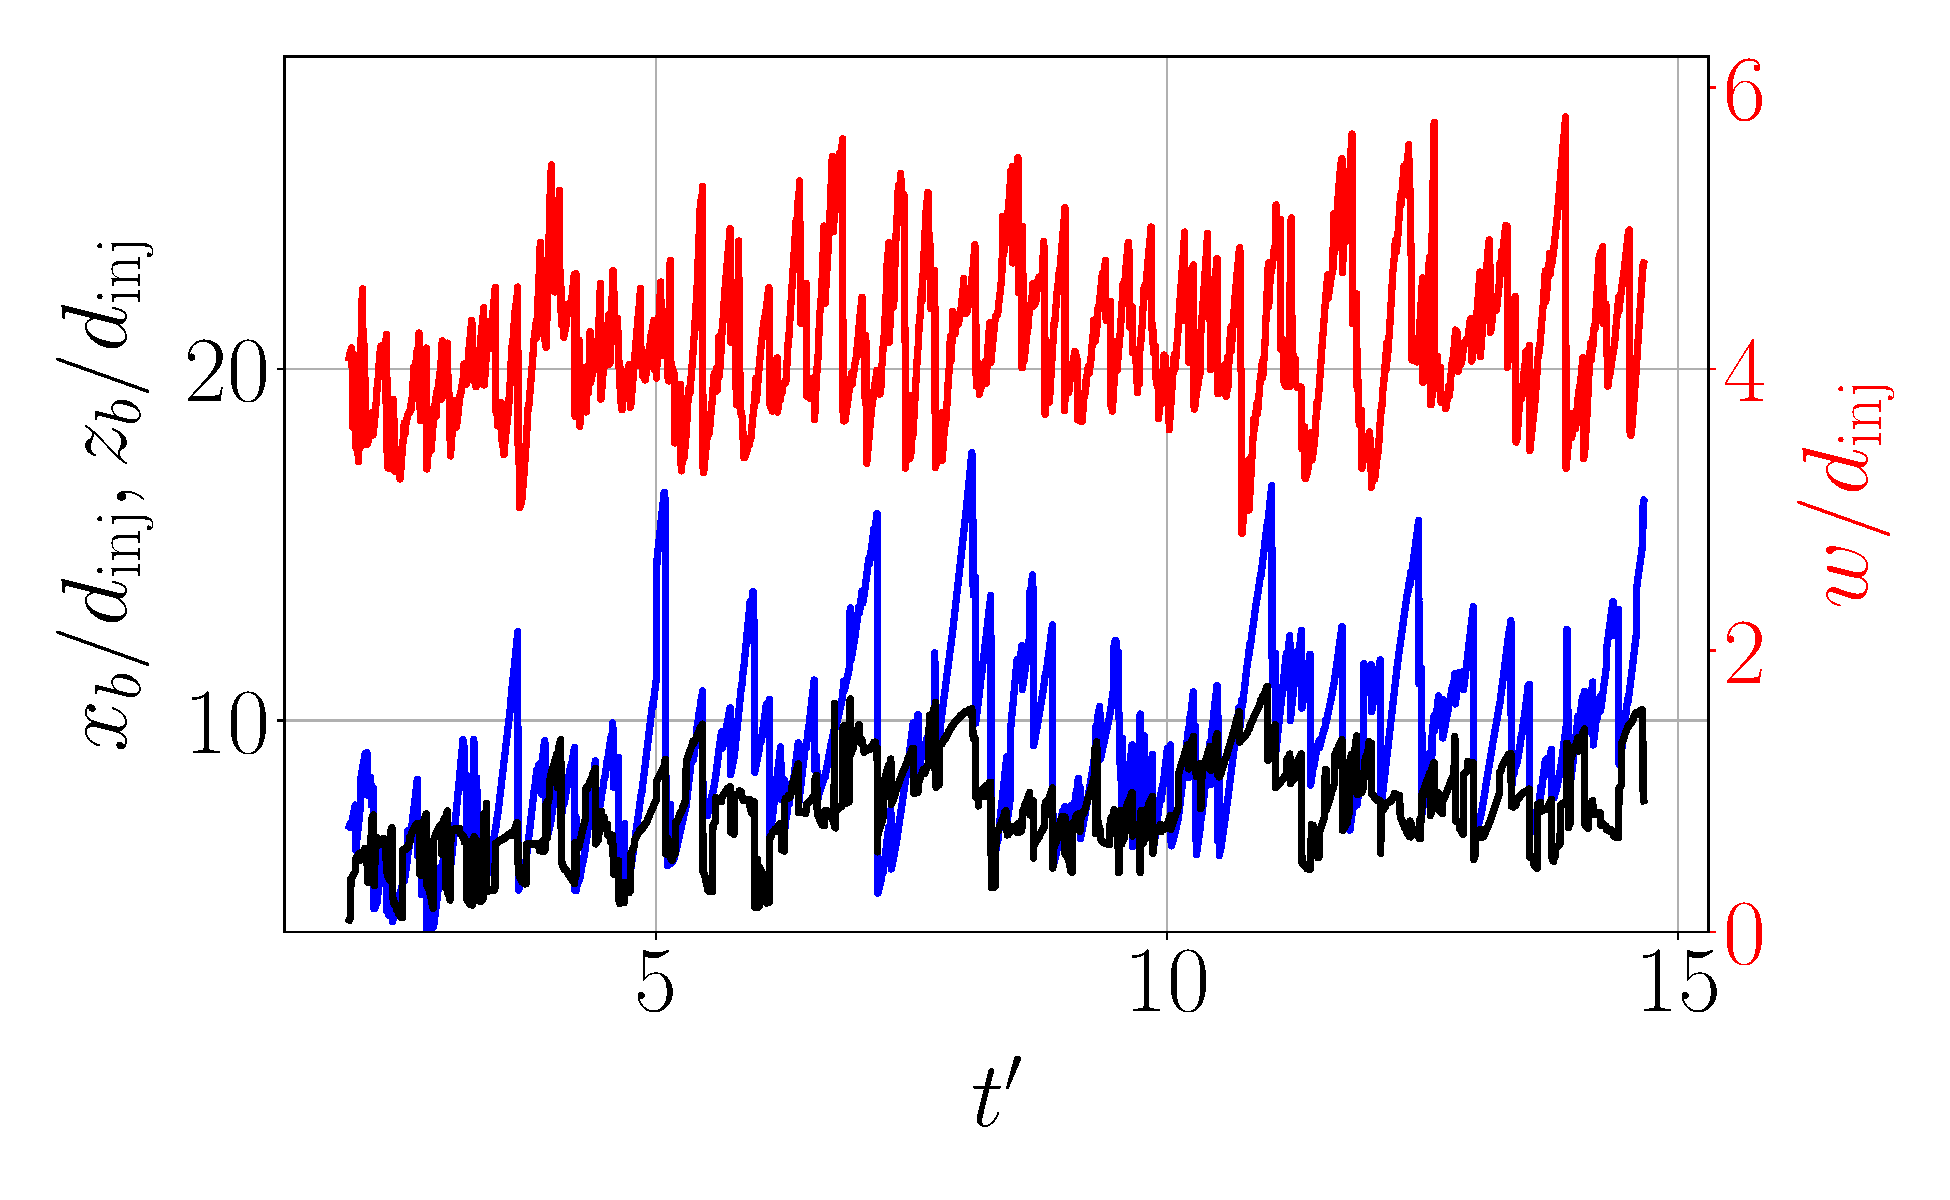
\includegraphics[scale=0.25]{./part2_developments/figures_ch5_resolved_JICF/results_dense_core_modeling/instant_xb_zb_w_UG75_DX20}
   \caption{Case UG75\_DX20}
   \label{fig:instant_xb_zb_w_UG75_DX20}
\end{subfigure}

\vskip\baselineskip

\begin{subfigure}[b]{0.45\textwidth}
	\centering
   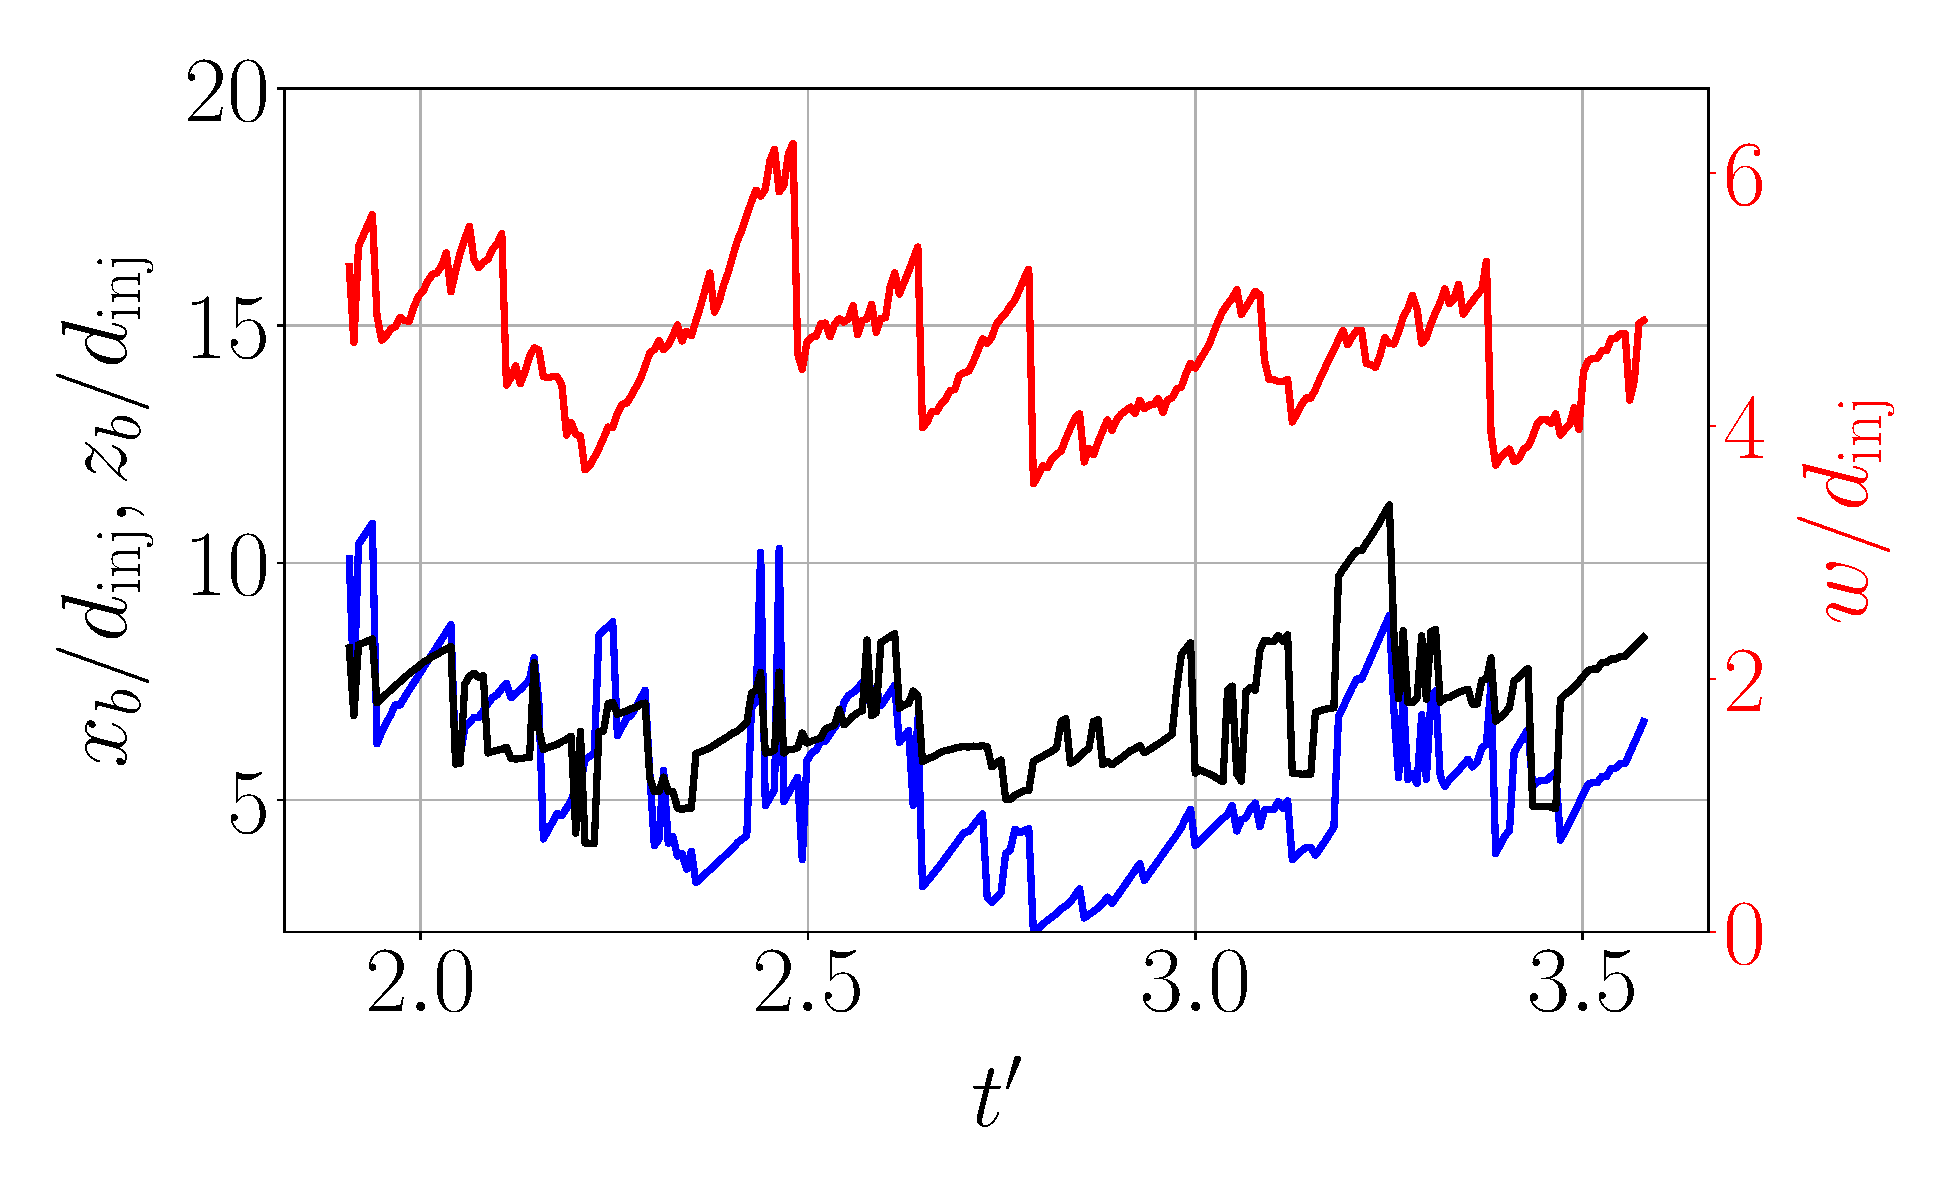
\includegraphics[scale=0.25]{./part2_developments/figures_ch5_resolved_JICF/results_dense_core_modeling/instant_xb_zb_w_UG100_DX10}
   \caption{Case UG100\_DX10}
   \label{fig:instant_xb_zb_w_UG100_DX10} 
\end{subfigure}
\hfill
\begin{subfigure}[b]{0.45\textwidth}
	\centering
   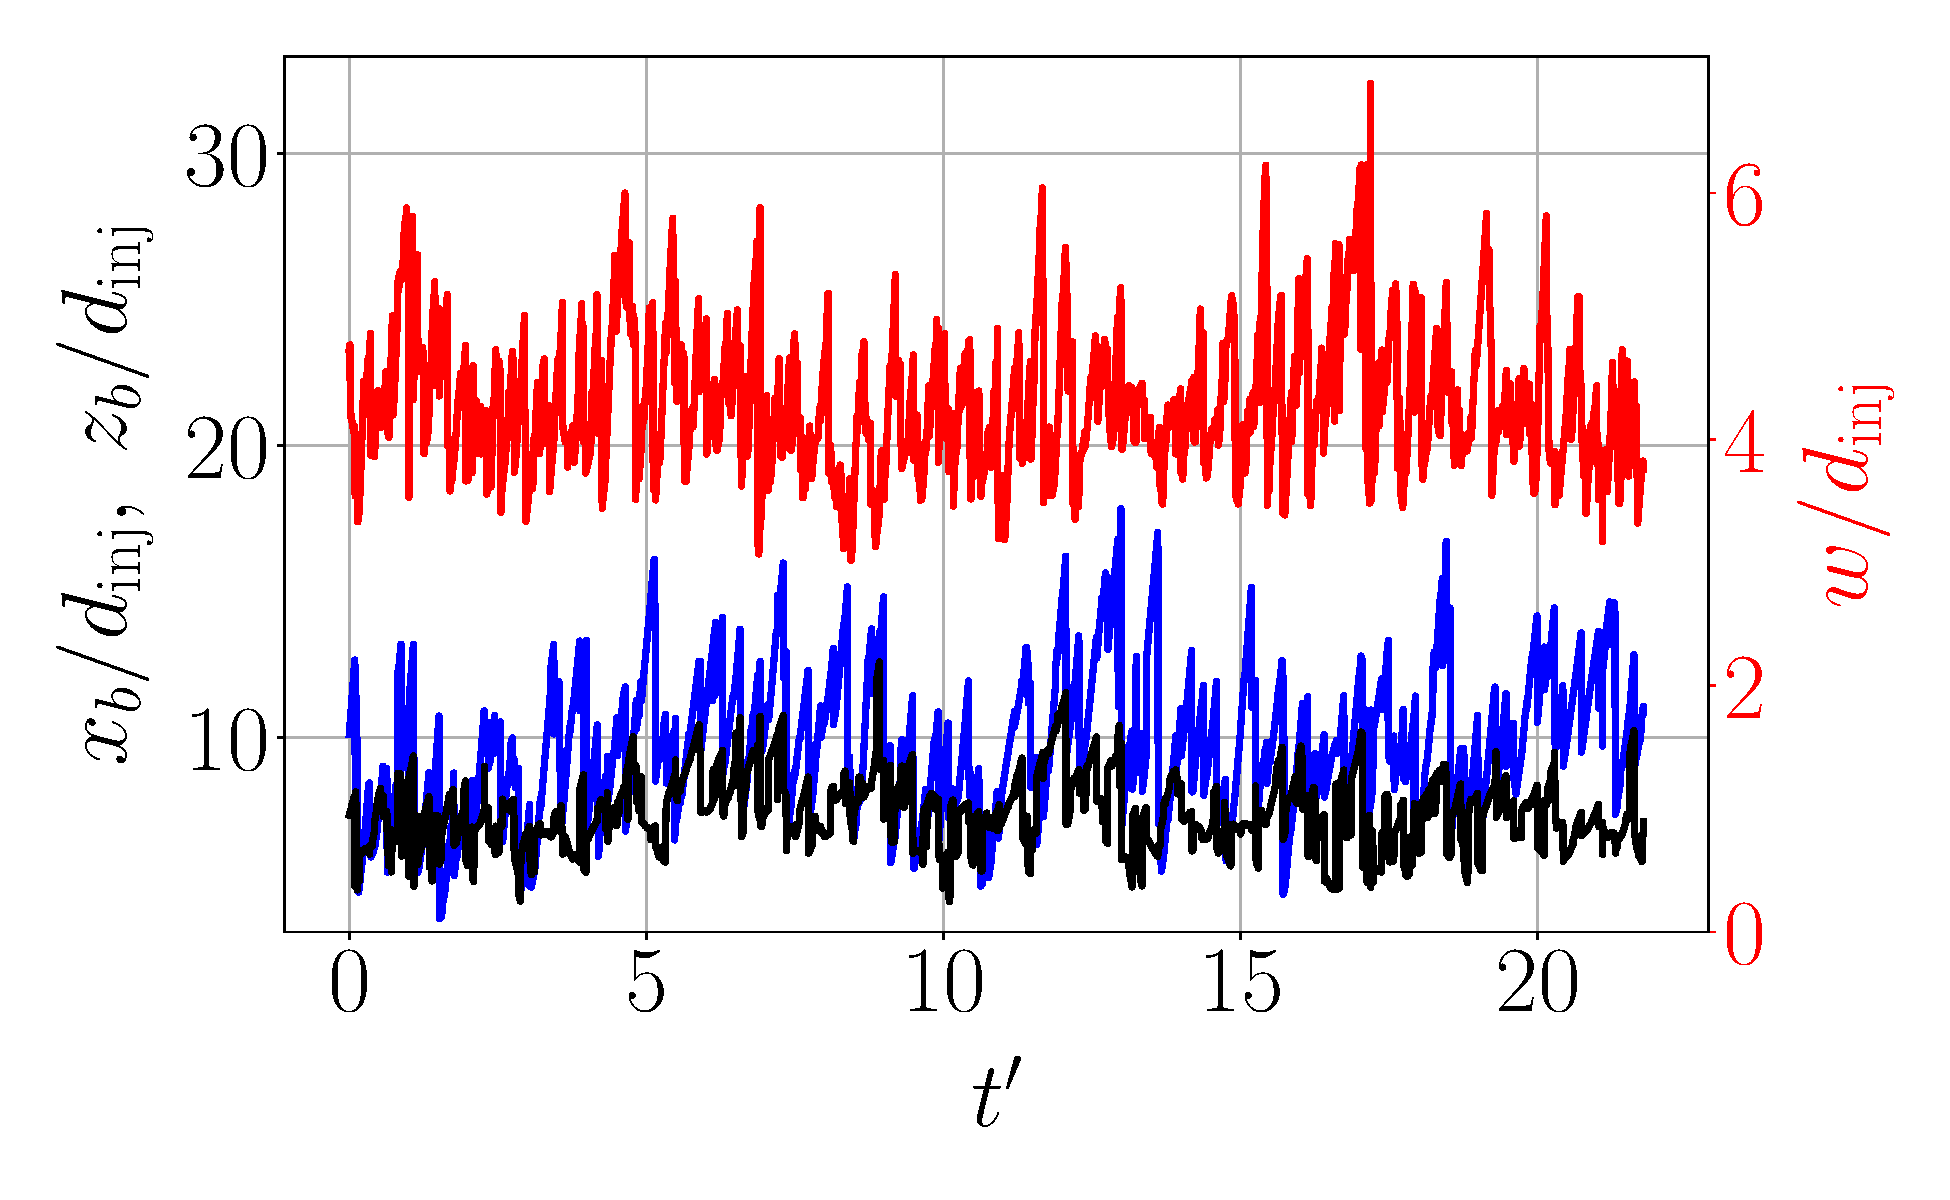
\includegraphics[scale=0.25]{./part2_developments/figures_ch5_resolved_JICF/results_dense_core_modeling/instant_xb_zb_w_UG100_DX20}
   \caption{Case UG100\_DX20}
   \label{fig:instant_xb_zb_w_UG100_DX20}
\end{subfigure}
   \caption{Variation with time of the dense core breakup point coordinates $x_\mathrm{b}, z_\mathrm{b}$ and width $w$.}

\label{fig:JICF_xb_zb_w_evolution}
\end{figure}

In order to define an actuator in the dispersed phase simulations represening the resolved dense core as accurate as possible, the mean values of the core coordinates and width will be used as input parameters for the model. For this purpose, the mean value of the signals from Figure \ref{fig:JICF_xb_zb_w_evolution} are calculated. The evolution of the mean values with time is shown in Figure \ref{fig:dense_core_mean_parameters_convergence}. As observed, the simulations performed with the coarse interface cell size $\Delta x_\mathrm{min} = 20~\mu m$ are converged for the three parameters $x_\mathrm{b}, z_\mathrm{b}$ and $w$. The fine resolutions $\Delta x_\mathrm{min} = 10~\mu m$ have not yet achieved full convergence due to its higher cost. The final mean values obtained are shown in the graphs of Figure \ref{fig:dense_core_mean_parameters_scatterplots}, which relate $z_\mathrm{b}$ and $w$ to $x_\mathrm{b}$. The bars in the figures denote the standard deviation of the instantaneous signals. Figure \ref{fig:dense_core_mean_parameters_scatterplots}a shows that the mean values for the coarse resolution are below the $\overline{z_\mathrm{b}} = \overline{x_\mathrm{b}}$, indicating that the dense core penetrates further along the streamwise direction $x$ than in the vertical $z$. On the contrary, the points for the fine resolution are located above this line, which shows that the dense core is elongated along the vertical direction. Yet, all parameters from the fine resolution simulations are lower than their respective ones of the coarse ones: primary breakup occurs previously for the former than for the latter. This is due to the presence of windwards instabilities in the fine simulations (which are not present in the coarse ones), which foster an earlier breakup.

\begin{figure}[ht]
\flushleft
\begin{subfigure}[b]{0.3\textwidth}
	\flushleft
   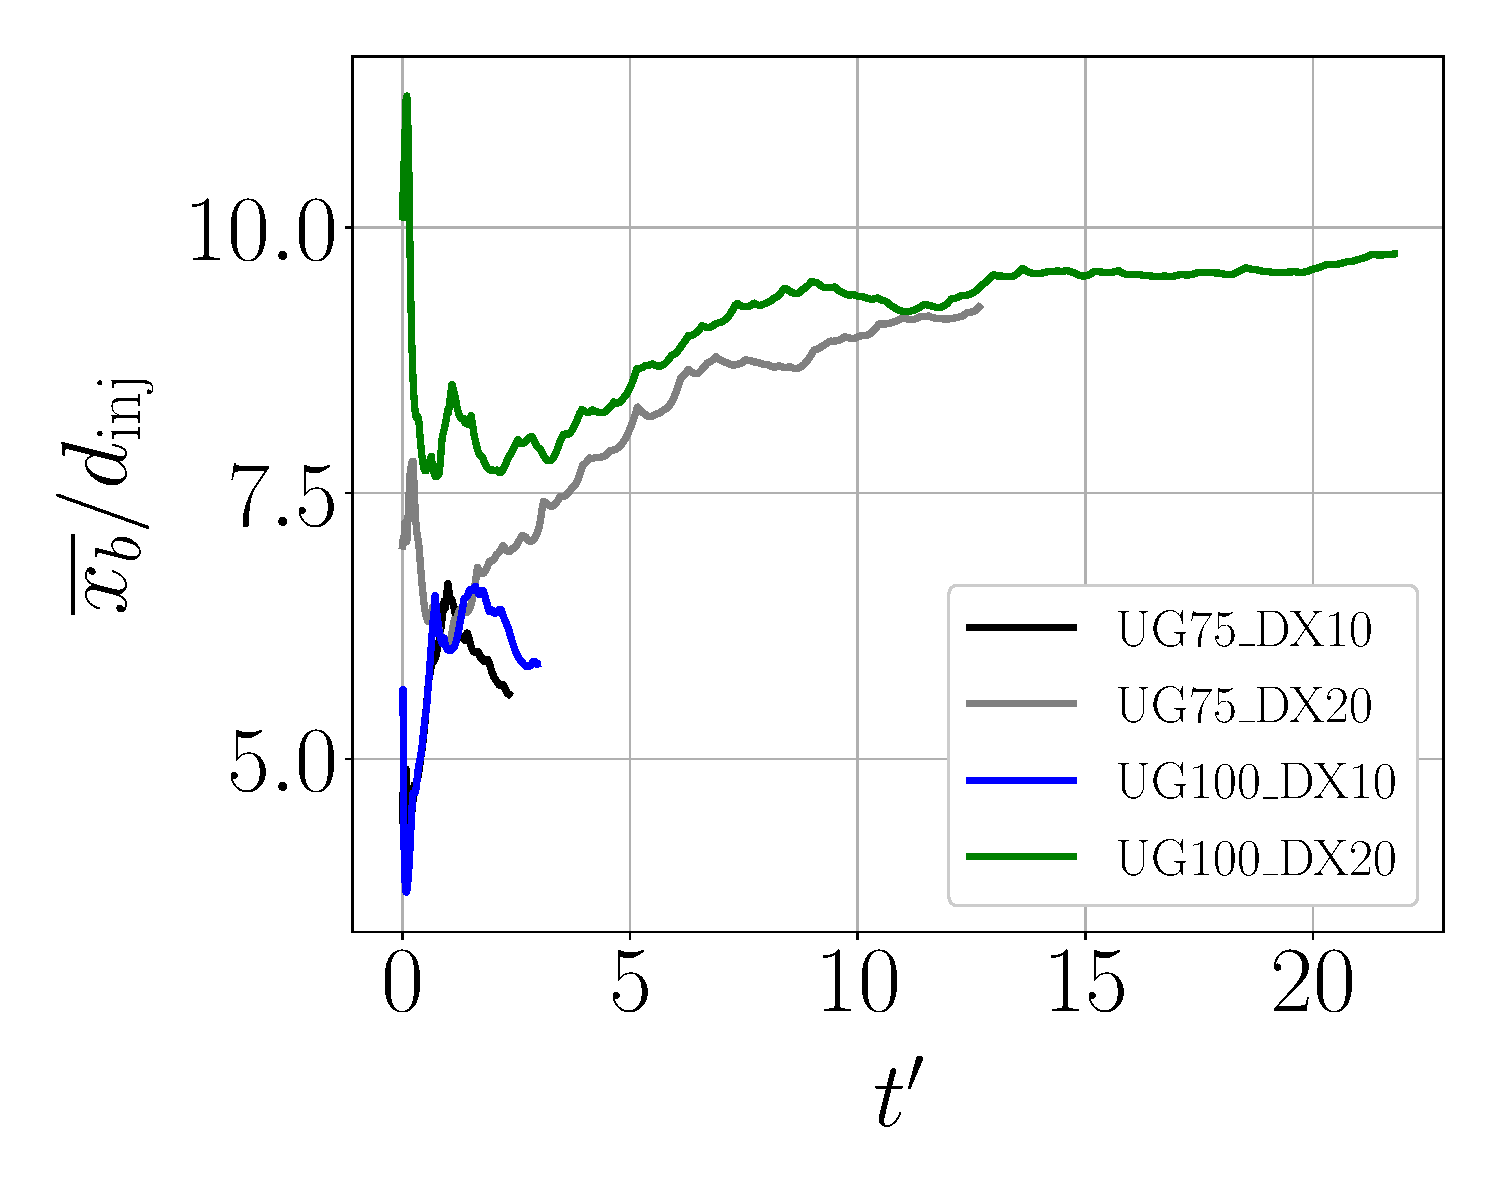
\includegraphics[scale=0.225]{./part2_developments/figures_ch5_resolved_JICF/results_dense_core_modeling/convergence_mean_xb}
\end{subfigure}
\hfill
\begin{subfigure}[b]{0.3\textwidth}
	\flushleft
   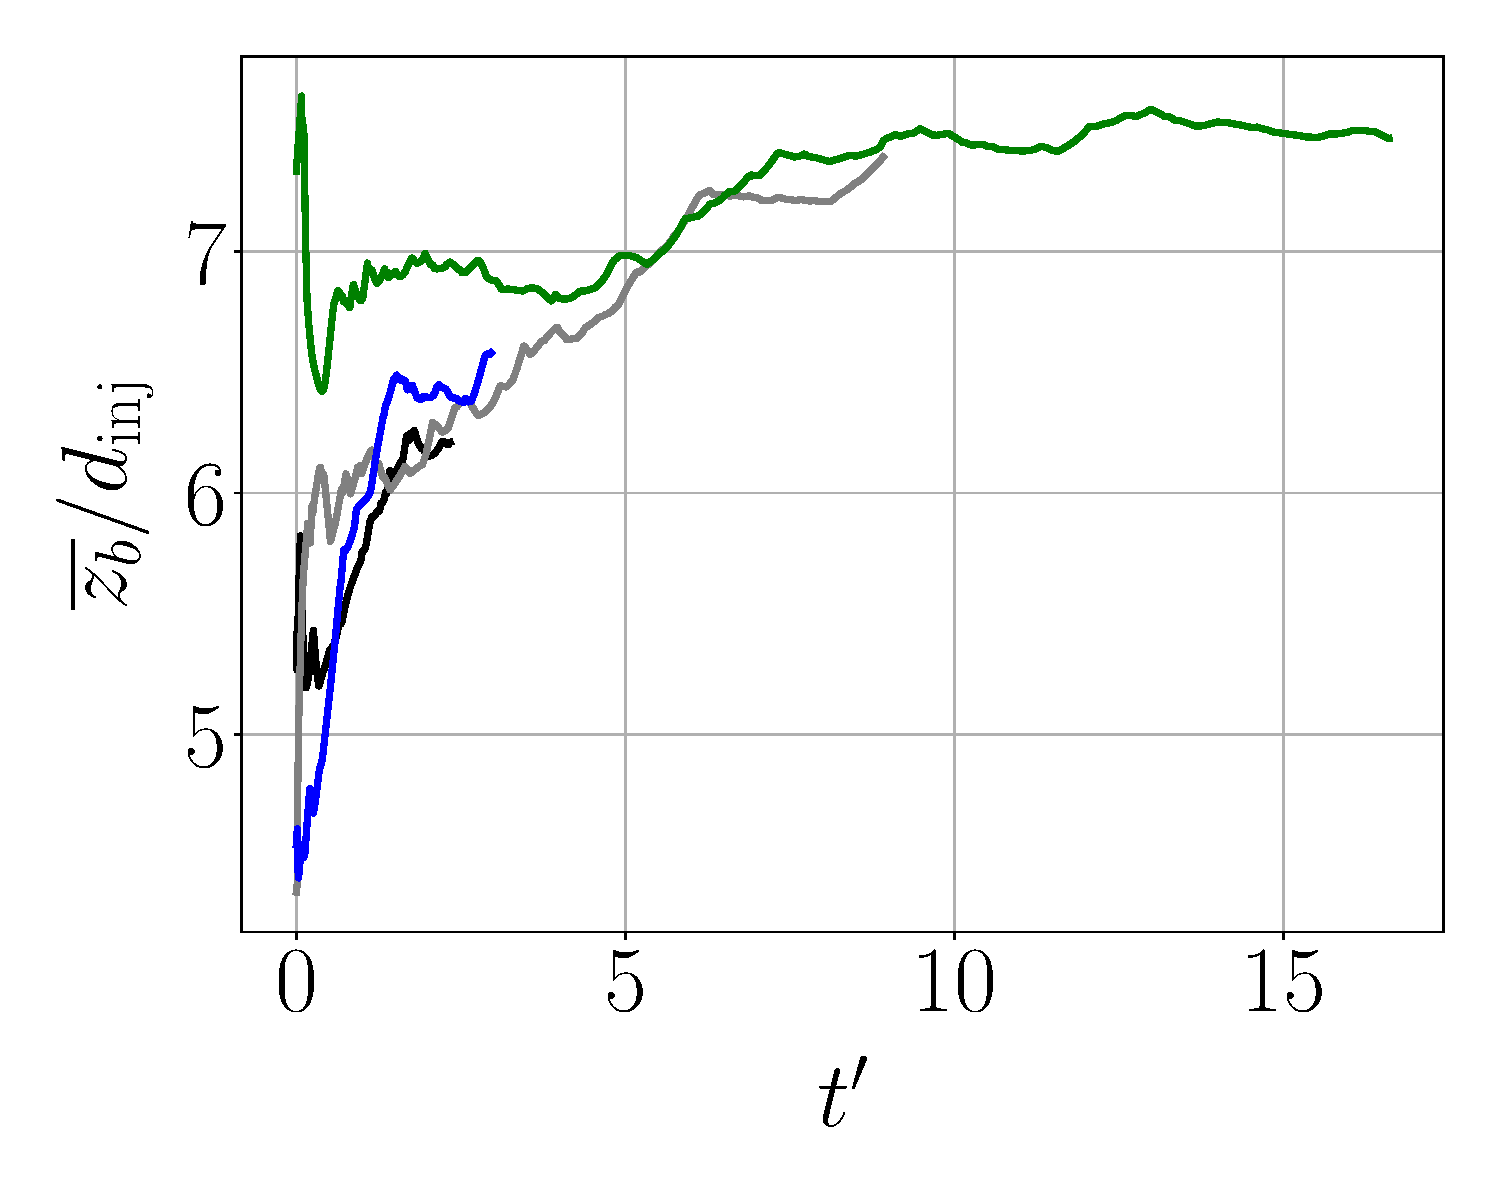
\includegraphics[scale=0.225]{./part2_developments/figures_ch5_resolved_JICF/results_dense_core_modeling/convergence_mean_zb}
\end{subfigure}
\hfill
\begin{subfigure}[b]{0.3\textwidth}
	\flushleft
   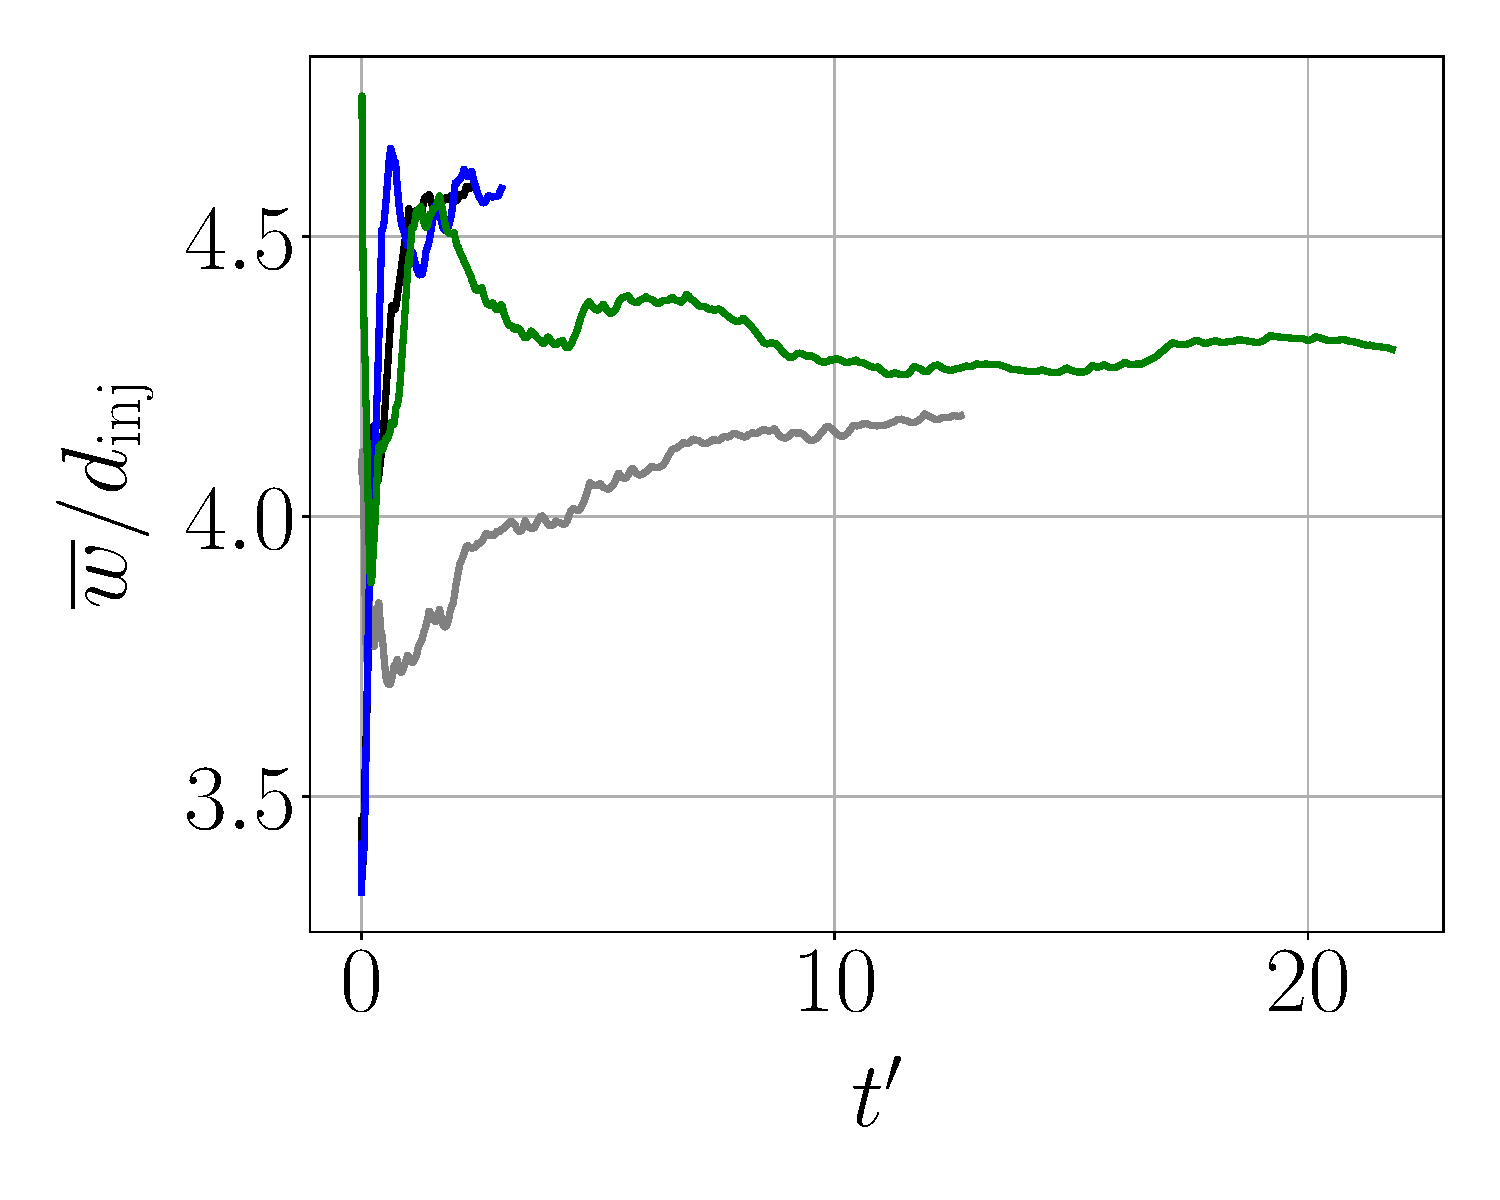
\includegraphics[scale=0.225]{./part2_developments/figures_ch5_resolved_JICF/results_dense_core_modeling/convergence_mean_width}
\end{subfigure}
   \caption{Evolution of mean geometric parameters of the dense core}
\label{fig:dense_core_mean_parameters_convergence}
\end{figure}

Figure \ref{fig:dense_core_mean_parameters_scatterplots} reveals also a dependendency of the mean parameters with respect to the operating conditions. The breakup coordinates $\overline{x_\mathrm{b}}$ and $\overline{z_\mathrm{b}}$ are lower for the low $We$ operating point: increasing aerodynamic gas forces pushes the breakup point further downstream and upper. This is coherent with the experimental results from \citeColor[patil_liquid_2021], who obtained a correlation for the axial breakup point which varies with the gas Weber number as $x_\mathrm{b} \propto We_g^{0.1}$. The dependency is on $We_g$ is however weak, as also found in Figure \ref{fig:dense_core_mean_parameters_scatterplots}a. This experimental study also includes a correlation for the width $w$ which is found to depend solely on the $q$ factor, which is also coherent with the results from Figure \ref{fig:dense_core_mean_parameters_scatterplots}b for the coarse resolution. The fine resolution shows a dependency of $w$ with the operating point: however, it is to bear in mind that the parameters from the fine resolutions are not fully converged, and therefore definitive conclusions cannot be extracted from these results. Further analysis would require running longer the fine simulations to reach convergence of the parameters. 


\begin{figure}[ht]
\flushleft
\begin{subfigure}[b]{0.45\textwidth}
	\centering
   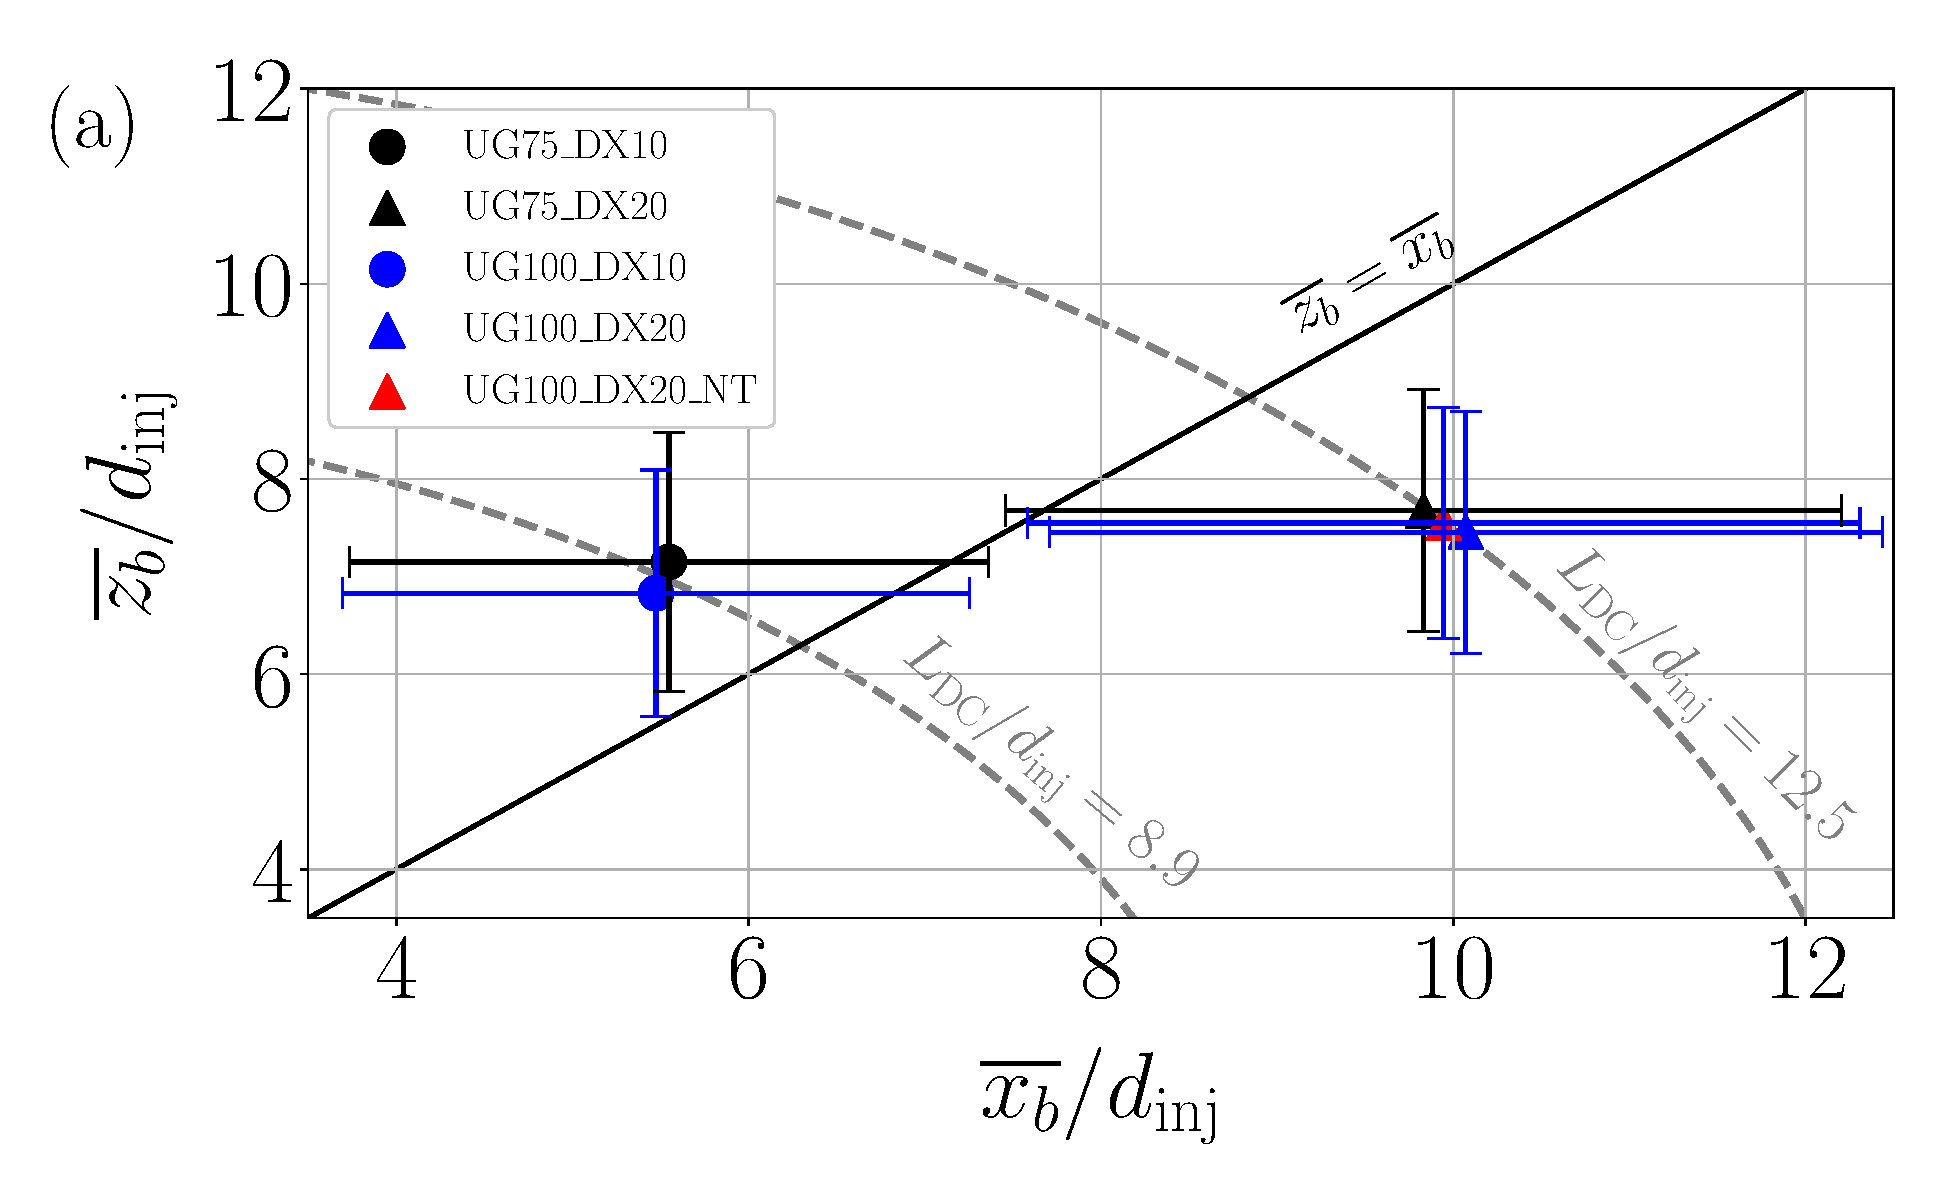
\includegraphics[scale=0.25]{./part2_developments/figures_ch5_resolved_JICF/results_dense_core_modeling/map_xb_zb}
   \label{fig:dense_core_mean_parameters_scatterplots_zb_xb}
\end{subfigure}
%\hfill
\hspace{0.25in}
\begin{subfigure}[b]{0.45\textwidth}
	\centering
   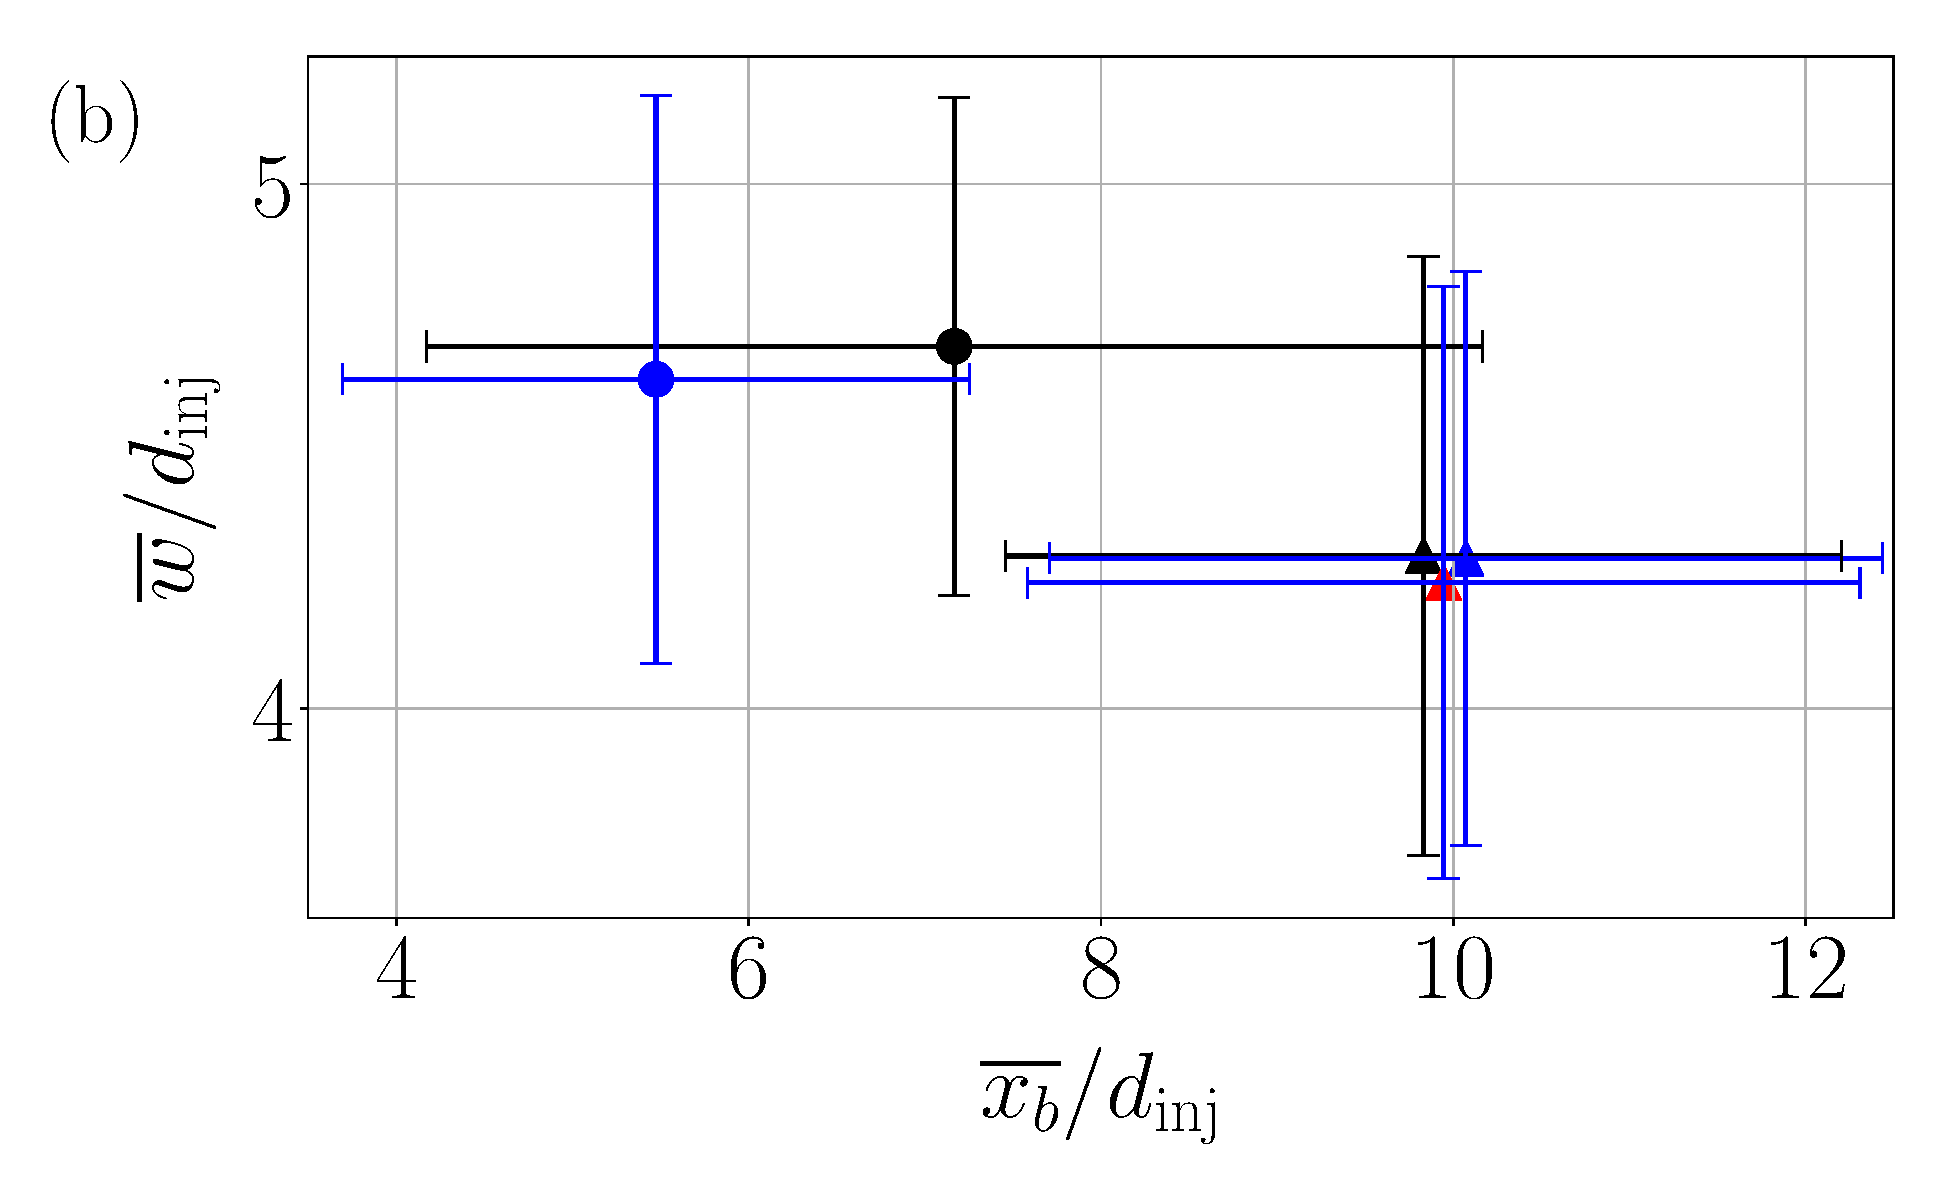
\includegraphics[scale=0.25]{./part2_developments/figures_ch5_resolved_JICF/results_dense_core_modeling/map_xb_width}
   \label{fig:dense_core_mean_parameters_scatterplots_w_xb}
\end{subfigure}
\caption{Mean values for the dense core geometric parameters}
\label{fig:dense_core_mean_parameters_scatterplots}
\end{figure}

%Patil correlations:
%
%\begin{equation}
%\frac{\overline{z_b}}{d_\mathrm{inj}} = 1.48 q^{0.3} We_g^{0.1} ~~~~; \frac{\overline{x_b}}{d_\mathrm{inj}} = 8.6 q^{-0.4}
%\end{equation}

\subsection{Turbulent structures in the gaseous field}
\label{ch5:subsec_turbulent_structures_in_gaseous_field}

Show here pictures of the iso-y, x and z planes with mean and RMS velocities (recirculation bubbles).

If possible, show Q-criterion.

Turbulent structures can be visualized with the Q-criterion \citeColor[jeong_identification_1995]:

\begin{equation}
Q = \frac{1}{2} \left( ||\pmb{\Omega}|| - ||\textbf{S}||^2 \right)
\end{equation}


\subsection{Defining pressure differences}
\label{ch5:subsec_defining_pressure_differences}

\clearpage

\section{Direct measurement of liquid fluxes}

The procedure proposed for obtainining liquid fluxes from the resolved simulations was described in $\S$\ref{subsec:ch5_interior_boundaries}. Liquid fluxes have been measured in the resolved simulations at the planes shown in Figure \ref{fig:jicf_interior_boundaries_surface_measurements}. In the simulations with a mesh resolution of $\Delta x_\mathrm{min} = 20 \mu m$, fluxes have been obtained in all interior boundaries (IBs) shown in the sketch, i.e. axial planes x = 5, 10 and 15 mm, and filming planes x < 5, 10 and 15 mm. For the fine simulations, results were collected up to x = 10 mm since the liquid was removed shortly afterwards to reduce the computational cost of the simulations. It is worth to mention that in the chosen JICF configuration, liquid is injected into the plenum through the nozzle in the $x$ direction. Then, the jet deviates towards the air streamwise direction $x$, and some liquid droplets will also hit the bottom wall which is perpendicular to the $z$ axis. Therefore, by mass conservation, the injected liquid flow rate (defined in Table \ref{tab:jicf_operating_conditions}) must be equal to the addition of the flow rates crossing an IB at a given $x$ location and a filming plane perpendicular to the $z$ axis which extends from downstream the injection nozzle up to the $x$ location of the vertical IB. This is equivalent to defining a rectangular control volume that encloses the full jet in the plenum up to a certain $x$ location: according to Eq. (\ref{eq:mass_conservation_general_bothPhases_transient}b), the flows entering the control volume (injected liquid) must be equal to the ones leaving it (ligaments or droplets flowing downstream and droplets reaching the walls). No other control surfaces need to be considered, since there is no liquid either flowing upstream of hitting the top or side walls.

Firstly, the overall flow rates in the interior boundaries are calculated. \st{These flow rates are compared to the ones obtained from the lagrangian tracking procedure}. It is shown that there is a reduction on the flow rate with axial distance, which is caused due to droplets resulting from atomization that reach the size of the mesh resolution and they disappear. This issue is adressed secondly in this section. Finally, fluxes are discretized to obtain a spatial distribution of the liquid flow rates, \st{which are also compared to the discretized fluxes obtained from the lagrangian tracking process}.

\subsection{Obtention of total flow rate}

The overall, or total, liquid flow rates are obtained in the IBs by applying Eq. (\ref{eq:Q_lIB_definition_with_Ne_and_No}). The IBs are firstly monitored at every time instant of the simulation. Figure \ref{fig:IB_liquid_flow_rate_inst_evolution_UG100_DX10} shows an example of instantaneous liquid flow rates $Q_l$ obtained from case UG100\_DX10. Two IBs perpendicular to the $x$ axis in the left image, and two filming IBs are shown in the right one. The injected flow rate into the domain, which is constant, is also plotted in the left figure as a dashed solid line. As observed, the fluxes in Figure \ref{fig:IB_liquid_flow_rate_inst_evolution_UG100_DX10} left show a high variation around the injected flow rate in both planes. This is due to an intermittent presence of liquid crossing the sampling planes once atomization has started taken place: the liquid phase is no longer a coherent jet but is composed by an ensemble of ligaments and droplets. At some time instants there will be big liquid structures or a high number of them (i.e. high volume of liquid) crossing a certain plane, hence the instantaneous flux can be larger than the injected flow rate. At other time instants this quantity will be lower, hence the instantaneous flux is smaller than the injected flow rate. This can be quantitatively check by looking at, for example, Figure \ref{fig:JICF_establishment_UG100_lateral}. Regarding the filming fluxes from Figure \ref{fig:IB_liquid_flow_rate_inst_evolution_UG100_DX10} right, these present lower magnitudes than the ones from the planes normal to the crossflow but still display a varying behaviour which, in some cases, can descend up to $0$. This is coherent, since the isntantaneous filming fluxes measure the quantity of liquid impinging the bottom wall at every time instant: in some cases there is no liquid reaching the wall, while in others there is a big quantity of droplets filming and creating the peaks of high $Q_l$ \hl{as the ones shown around $t^{\prime} \sim 1$ in the corresponding figure}.

Due to the intermittent behaviour of the flow rates, the instantaneous fluxes are not useful to characterize the flow rates in the IBs. Instead, the mean flow rates must be obtained. 

The evolution of the mean and RMS values of IBs flow rates with time is shown in Figure \ref{fig:IB_mean_RMS_Ql_evolution}.

Mean values are shown in Figure \ref{fig:IB_bargraph}.

\clearpage

\begin{figure}[ht]
\flushleft
\begin{subfigure}[b]{0.45\textwidth}
	\centering
   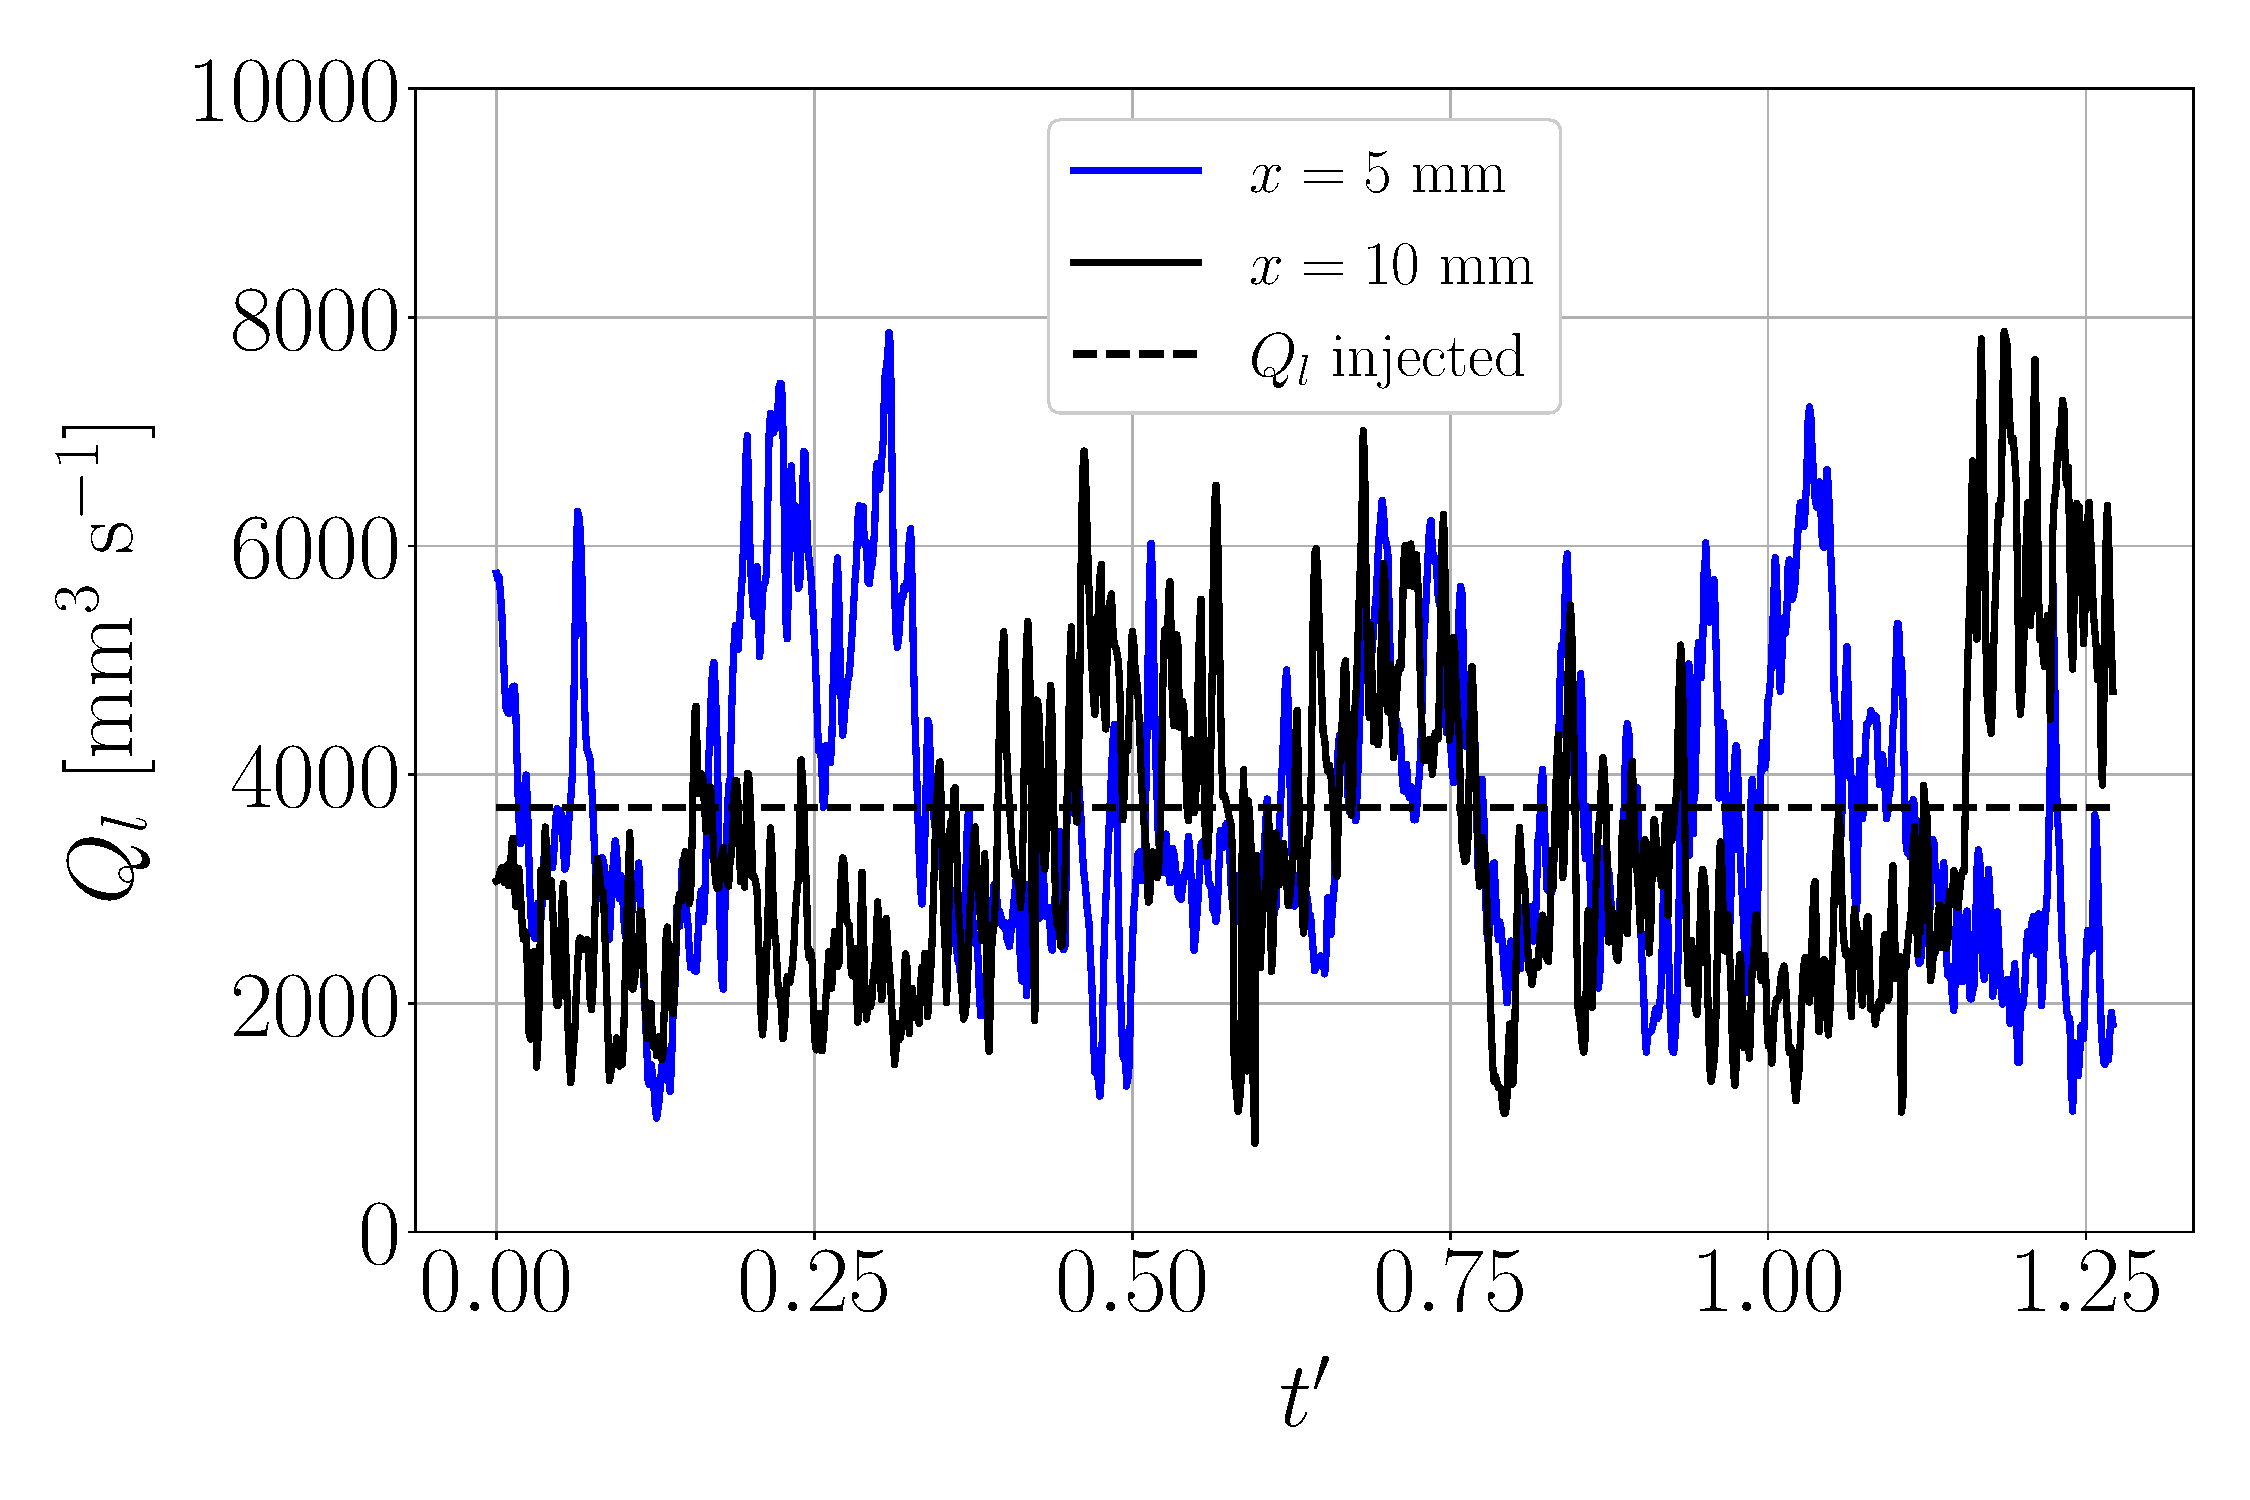
\includegraphics[scale=0.225]{./part2_developments/figures_ch5_resolved_JICF/flow_rates_ibs/inst_Q_iso_x_UG100_dx10}
   %\caption{}
   %\label{} 
\end{subfigure}
\hspace{0.4in}
\begin{subfigure}[b]{0.45\textwidth}
	\centering
   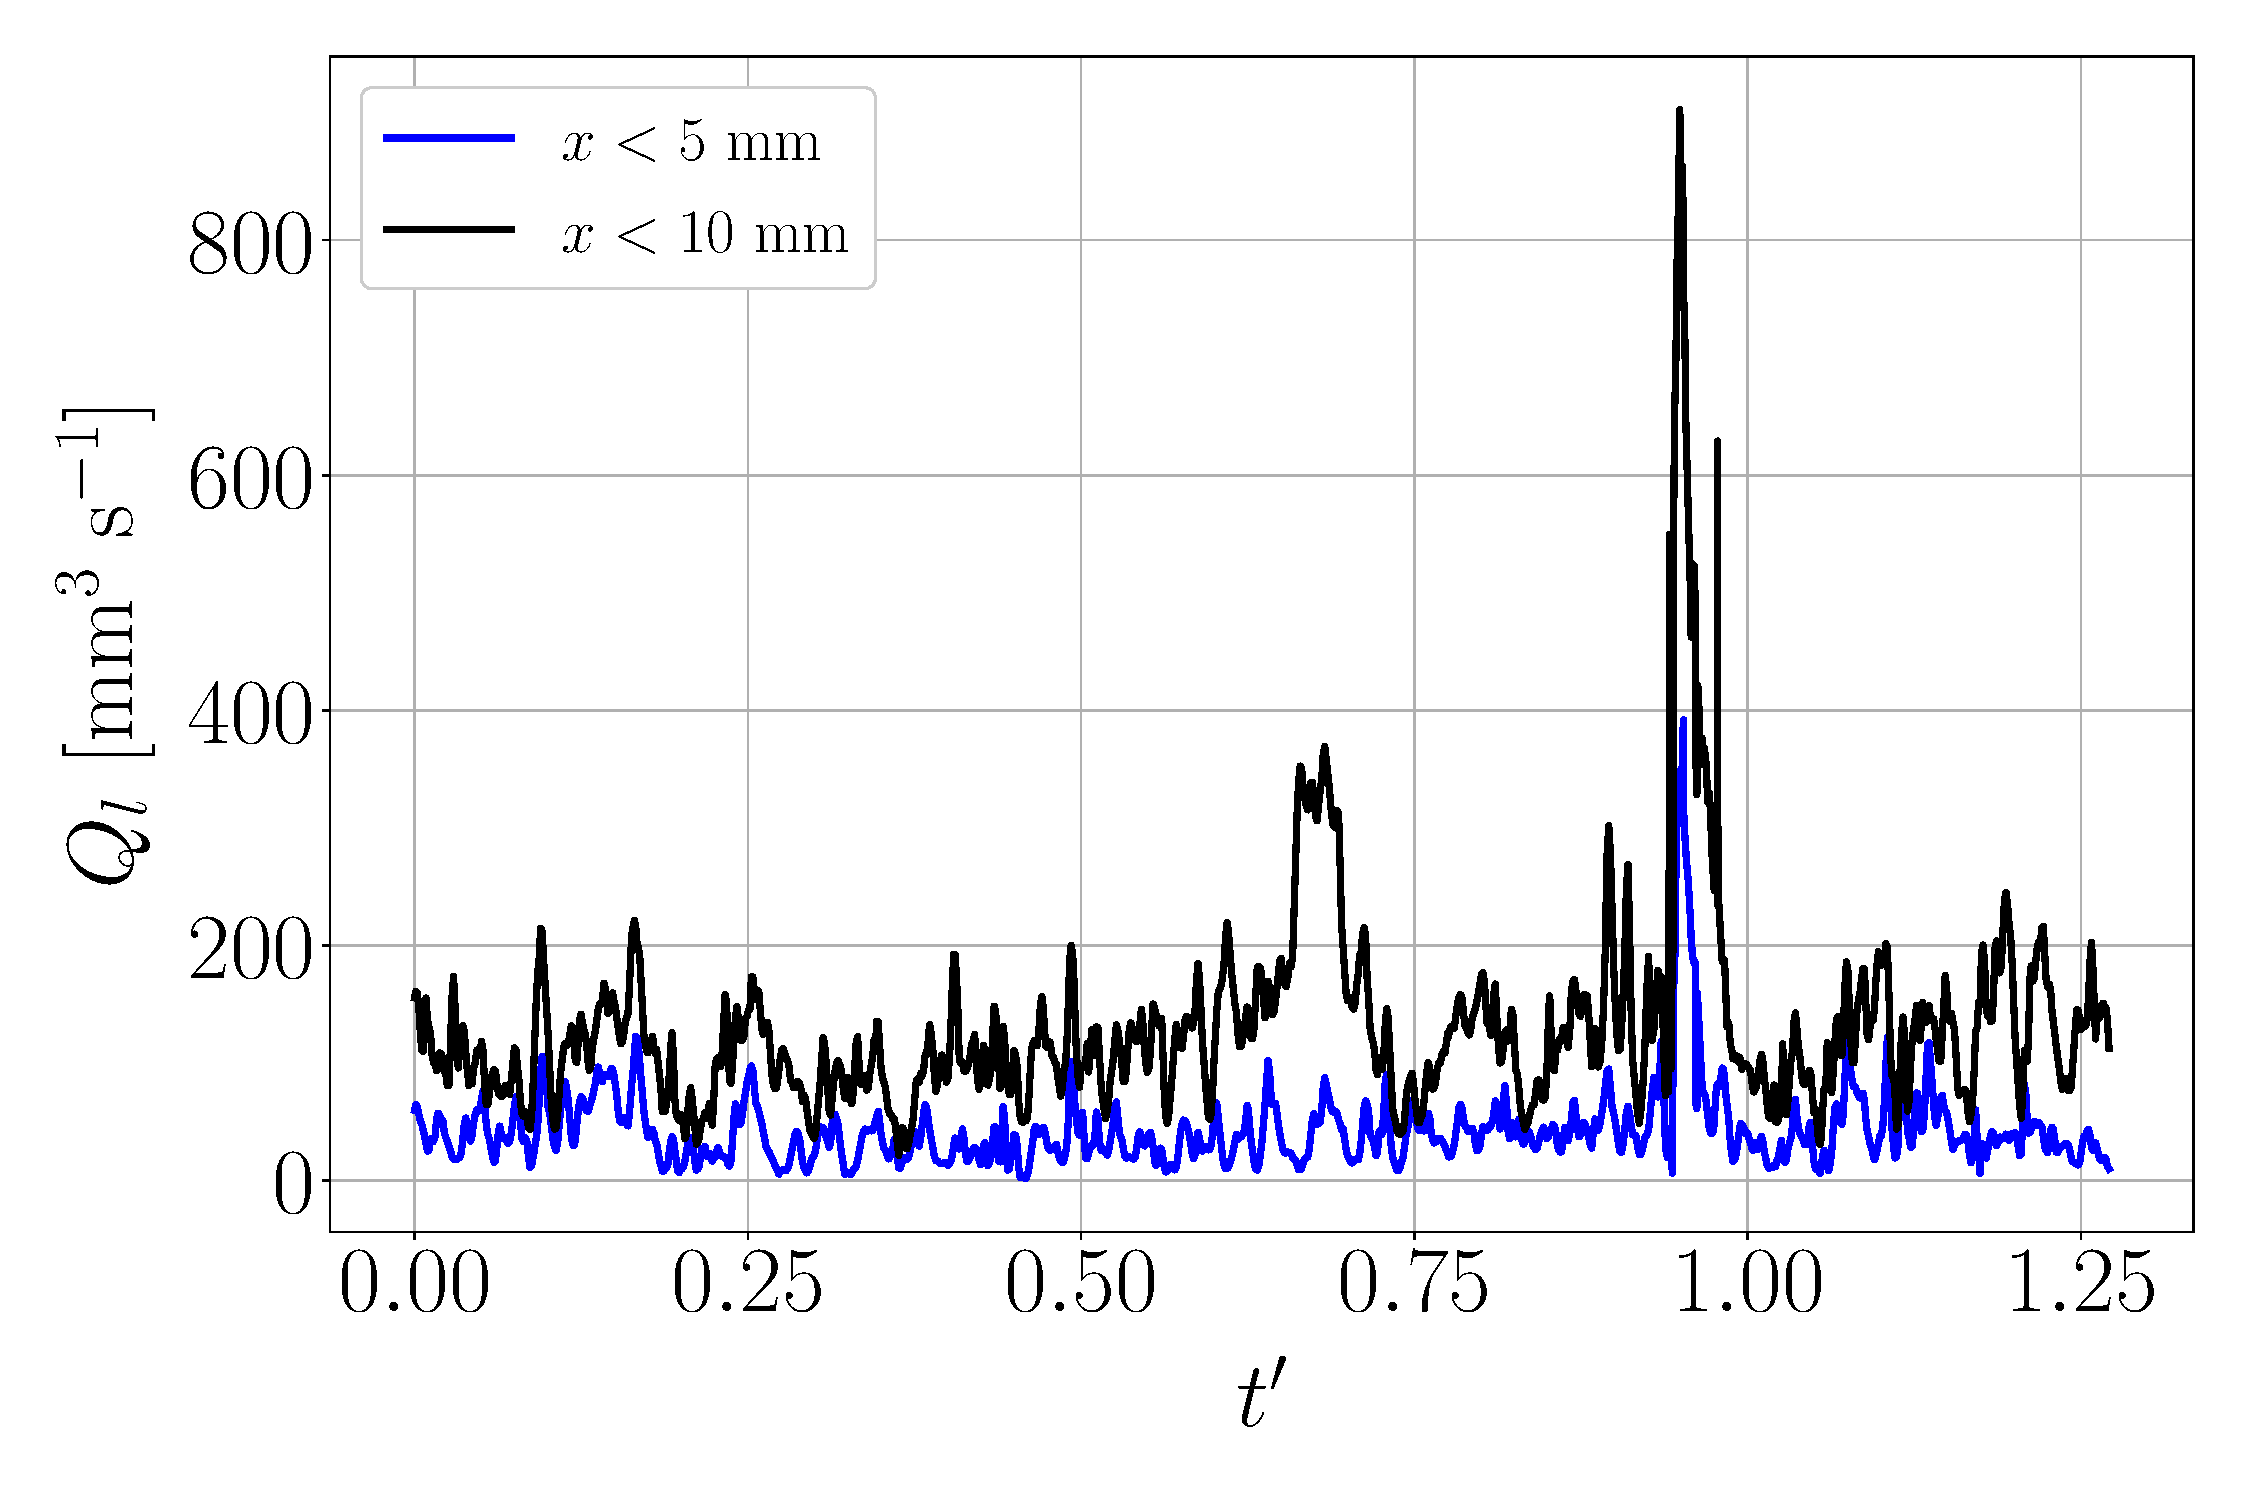
\includegraphics[scale=0.225]{./part2_developments/figures_ch5_resolved_JICF/flow_rates_ibs/inst_Q_iso_x_UG100_dx10_filming}
   %\caption{}
   %\label{}
\end{subfigure}
\caption[Instantaneous liquid flow rates $Q_l$ for case UG100\_DX10.]{Time evolution of instantaneous liquid flow rates $Q_l$ for case UG100\_DX10. \textsl{Left}: planes normal to crossflow. \textsl{Right}: filming planes.}
\label{fig:IB_liquid_flow_rate_inst_evolution_UG100_DX10}
\end{figure}


\begin{figure}[ht]
\flushleft
\begin{subfigure}[b]{0.9\textwidth}
	\flushleft
   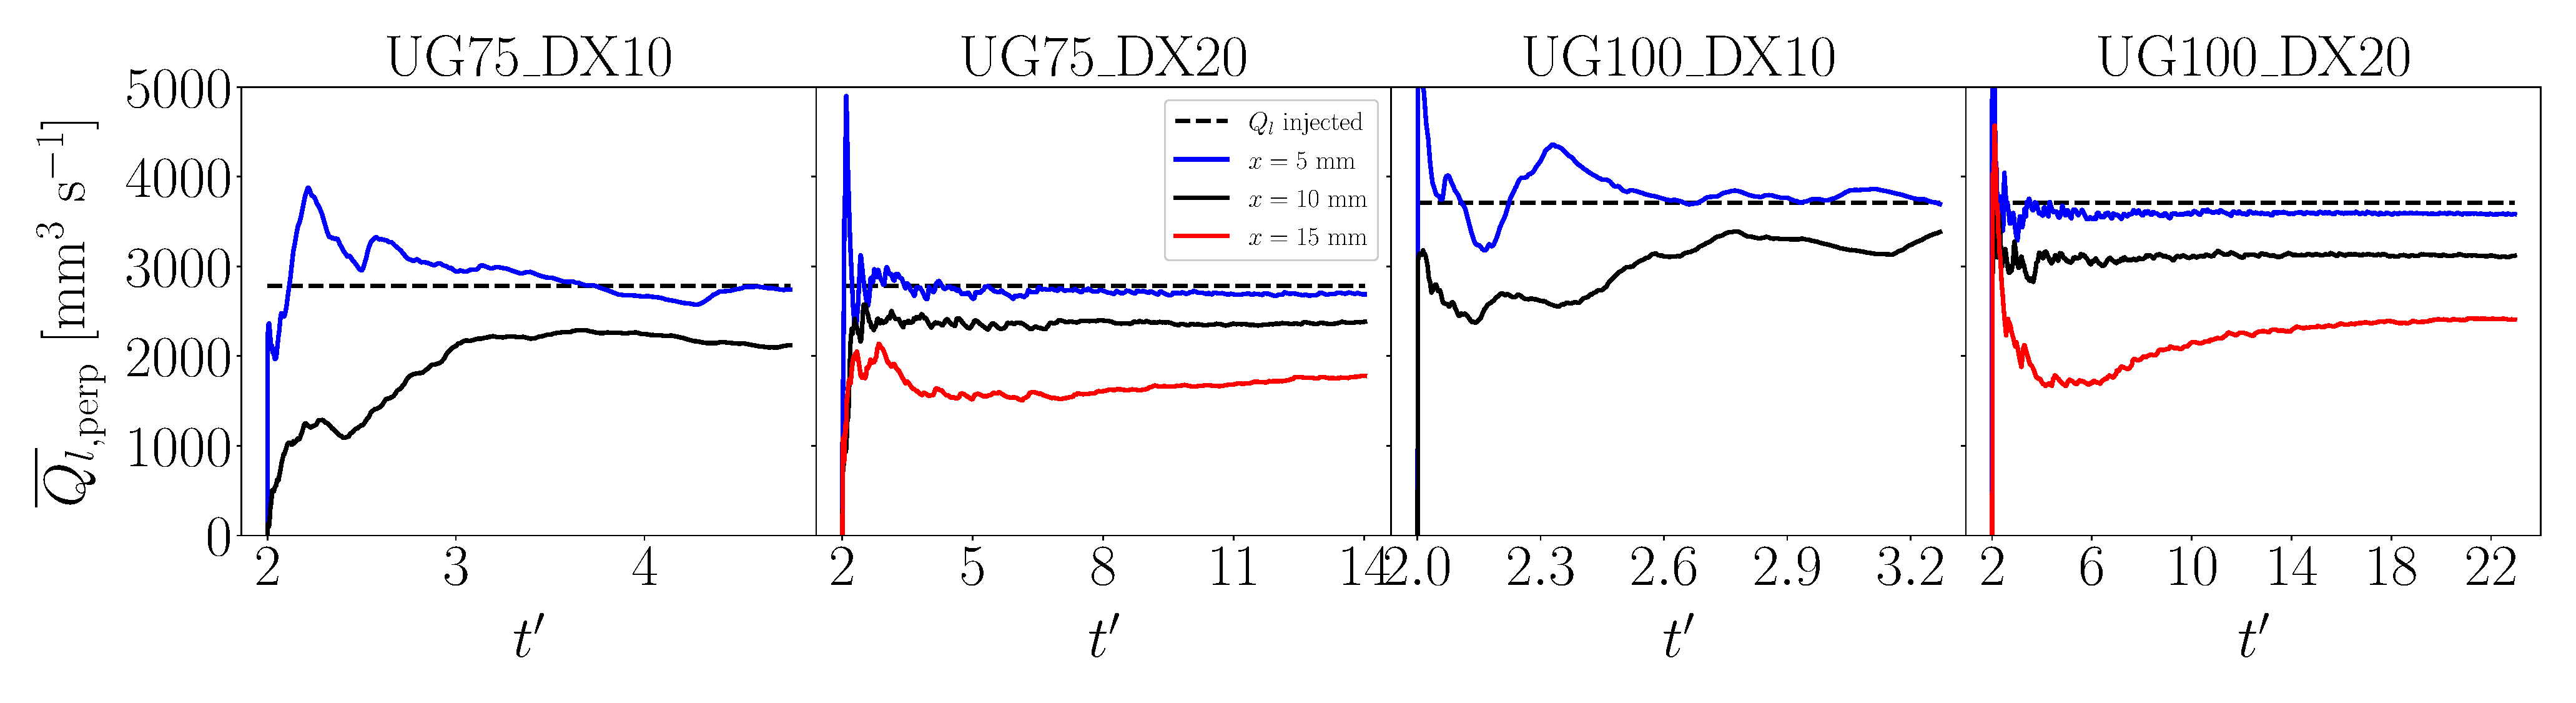
\includegraphics[scale=0.25]{./part2_developments/figures_ch5_resolved_JICF/flow_rates_ibs/evolution_mean_Q_iso_x}
   \caption{Mean $Q_l$ evolution in IBs perpendicular to crossflow.}
   %\label{} 
\end{subfigure}

\vskip\baselineskip

\begin{subfigure}[b]{0.9\textwidth}
	\flushleft
   \includegraphics[scale=0.25]{./part2_developments/figures_ch5_resolved_JICF/flow_rates_ibs/evolution_rms_Q_iso_x}
   \caption{RMS $Q_l$ evolution in IBs perpendicular to crossflow.}
   %\label{}
\end{subfigure}

\vskip\baselineskip

\begin{subfigure}[b]{0.9\textwidth}
	\flushleft
   \includegraphics[scale=0.25]{./part2_developments/figures_ch5_resolved_JICF/flow_rates_ibs/evolution_mean_Q_filming}
   \caption{Mean $Q_l$ evolution in filming IBs.}
   %\label{} 
\end{subfigure}

\vskip\baselineskip

\begin{subfigure}[b]{0.9\textwidth}
	\flushleft
   \includegraphics[scale=0.25]{./part2_developments/figures_ch5_resolved_JICF/flow_rates_ibs/evolution_rms_Q_iso_x}
   \caption{RMS $Q_l$ evolution in filming IBs.}
   %\label{}
\end{subfigure}
\caption{Time evolution of mean and RMS values of $Q_l$ in IBs}
\label{fig:IB_mean_RMS_Ql_evolution}
\end{figure}

\clearpage


\begin{figure}[ht]
\flushleft
\begin{subfigure}[b]{0.9\textwidth}
	\flushleft
   \includegraphics[scale=0.25]{./part2_developments/figures_ch5_resolved_JICF/flow_rates_ibs/bar_graph_isox_IBs}
   \caption{IBs perpendicular to crossflow.}
   %\label{} 
\end{subfigure}

\vskip\baselineskip

\begin{subfigure}[b]{0.9\textwidth}
	\flushleft
   \includegraphics[scale=0.25]{./part2_developments/figures_ch5_resolved_JICF/flow_rates_ibs/bar_graph_filming_IBs}
   \caption{Filming IBs}
   %\label{}
\end{subfigure}
\caption{Mean flow rates (bars) and RMS (black vertical lines) obtained with IBs for each simulation.}
\label{fig:IB_bargraph}
\end{figure}


%
%\begin{figure}[ht]
%\centering
%\begin{subfigure}[b]{0.45\textwidth}
%	\centering
%   \includegraphics[scale=0.17]{./part2_developments/figures_ch5_resolved_JICF/flow_rates_ibs/uG100_dx20_QL_isox_mean_time_convergence.eps}
%   \caption{Mean $Q_l$ in crossflow planes}
%   %\label{} 
%\end{subfigure}
%\hfill
%\begin{subfigure}[b]{0.45\textwidth}
%	\centering
%   \includegraphics[scale=0.17]{./part2_developments/figures_ch5_resolved_JICF/flow_rates_ibs/uG100_dx20_QL_isox_RMS_time_convergence.eps}
%   \caption{RMS $Q_l$ in crossflow planes}
%   %\label{}
%\end{subfigure}
%\vskip\baselineskip
%\begin{subfigure}[b]{0.45\textwidth}
%	\centering
%   \includegraphics[scale=0.17]{./part2_developments/figures_ch5_resolved_JICF/flow_rates_ibs/uG100_dx20_QL_filming_mean_time_convergence.eps}
%   \caption{Mean $Q_l$ in filming planes}
%   %\label{} 
%\end{subfigure}
%\hfill
%\begin{subfigure}[b]{0.45\textwidth}
%	\centering
%   \includegraphics[scale=0.17]{./part2_developments/figures_ch5_resolved_JICF/flow_rates_ibs/uG100_dx20_QL_filming_RMS_time_convergence.eps}
%   \caption{RMS $Q_l$ in filming planes}
%   %\label{}
%\end{subfigure}
%\caption{Time evolution of mean and RMS liquid flow rates for case UG100\_DX20.}
%\label{fig:IB_liquid_flow_rate_mean_RMS_evolution_UG100_DX20}
%\end{figure}
%
%\newpage
%
%\begin{figure}[ht]
%\centering
%\begin{subfigure}[b]{0.45\textwidth}
%	\centering
%   \includegraphics[scale=0.10]{./part2_developments/figures_ch5_resolved_JICF/flow_rates_ibs/uG100_dx20_QL_isox_bar_plot.eps}
%   \caption{Case UG100\_DX20: crossflow planes}
%   %\label{} 
%\end{subfigure}
%\hfill
%\begin{subfigure}[b]{0.45\textwidth}
%	\centering
%   \includegraphics[scale=0.10]{./part2_developments/figures_ch5_resolved_JICF/flow_rates_ibs/uG100_dx20_QL_filming_bar_plot.eps}
%   \caption{Case UG100\_DX20: filming planes}
%   %\label{}
%\end{subfigure}
%\vskip\baselineskip
%\begin{subfigure}[b]{0.45\textwidth}
%	\centering
%   \includegraphics[scale=0.10]{./part2_developments/figures_ch5_resolved_JICF/flow_rates_ibs/uG100_dx10_QL_isox_bar_plot.eps}
%   \caption{Case UG100\_DX10: crossflow planes}
%   %\label{} 
%\end{subfigure}
%\hfill
%\begin{subfigure}[b]{0.45\textwidth}
%	\centering
%   \includegraphics[scale=0.10]{./part2_developments/figures_ch5_resolved_JICF/flow_rates_ibs/uG100_dx10_QL_filming_bar_plot.eps}
%   \caption{Case UG100\_DX10: filming planes}
%   %\label{}
%\end{subfigure}
%
%\vskip\baselineskip
%
%\begin{subfigure}[b]{0.45\textwidth}
%	\centering
%   \includegraphics[scale=0.10]{./part2_developments/figures_ch5_resolved_JICF/flow_rates_ibs/uG75_dx20_QL_isox_bar_plot.eps}
%   \caption{Case UG75\_DX20: crossflow planes}
%   %\label{} 
%\end{subfigure}
%\hfill
%\begin{subfigure}[b]{0.45\textwidth}
%	\centering
%   \includegraphics[scale=0.10]{./part2_developments/figures_ch5_resolved_JICF/flow_rates_ibs/uG75_dx20_QL_filming_bar_plot.eps}
%   \caption{Case UG75\_DX20: filming planes}
%   %\label{}
%\end{subfigure}
%\vskip\baselineskip
%\begin{subfigure}[b]{0.45\textwidth}
%	\centering
%   \includegraphics[scale=0.10]{./part2_developments/figures_ch5_resolved_JICF/flow_rates_ibs/uG75_dx10_QL_isox_bar_plot.eps}
%   \caption{Case UG75\_DX10: crossflow planes}
%   %\label{} 
%\end{subfigure}
%\hfill
%\begin{subfigure}[b]{0.45\textwidth}
%	\centering
%   \includegraphics[scale=0.10]{./part2_developments/figures_ch5_resolved_JICF/flow_rates_ibs/uG75_dx10_QL_filming_bar_plot.eps}
%   \caption{Case UG75\_DX10: filming planes}
%   %\label{}
%\end{subfigure}
%\caption[Mean flow rates (bars) and RMS (lines) obtained with interior boundaries for each simulation performed]{Mean flow rates (bars) and RMS (lines) obtained with interior boundaries for each simulation performed. }
%\label{fig:JICF_ibs_flow_rates_bars_plots}
%\end{figure}

\clearpage





\subsection{Mass conservation in ACLS}
\label{subsec:ch5_mass_conservation_ACLS_set_levelset_band}




\subsection{Spatial distribution of flow rates in crossflow planes}




%\subsubsection{Sampling procedure for droplets}

\newpage

\section{Spray characterization}
\label{sec:ch5_sec_spray_characterization}

The number of droplets accumulated in each sampling plane for all the simulations performed in shown in Figure \ref{tab:jicf_Ndr_accumulated}.

\begin{table}[!h]
\centering
\caption{Number of droplets accumulated in JICF simulations}
\begin{tabular}{rcccc}
\thickhline
\textbf{Case} & $x = 5$ mm & $x = 10$ mm & $x = 15$ mm  & $x = 20$ mm \\
\thickhline 
UG75\_DX10  & 14233 & 20677 & - & - \\
UG75\_DX20  &  6882 & 12224 & 12077 & 9440 \\
UG100\_DX10 & 16442 & 11087 & - & -\\
UG100\_DX20 & 21824 & 17793 & 9476 & 11041 \\
\thickhline
\end{tabular}
\label{tab:jicf_Ndr_accumulated}
\end{table}

For the histograms, we can see 2013 Vie.


\subsection{Deformation variation with axial distance}

\subsection{Granulometry}

Sprays generated by atomization processes can be characterized by means of distributions. A given spray where the sizes of the droplets are known can be studied by representing distributions which express the probability of finding a droplet diameter or volume in that spray. Size distributions are usually representing by the notation $f_0 \left( D \right)$, while volume distributions are denoted by $f_3 \left( D \right)$. Two types of distributions are possible: discrete (histograms) or continuous. In the former, the spectrum of droplets size is divided into several range of droplets named bins or classes, and the number of droplets comprised within each class each counted. Histograms are the usual way of representing the granulometry when the size of droplets is directly available, such as in most experimental campaings and computational studies resolving atomization. Continuous distributions, however, are often used to fit discrete distributions obtained experimentally and are used for making simplified models for spray injection in lagrangian simulations, since they can represent the spray by functions depending on few parameters. Examples of function widely used in sprays are the lognormal, Rosin-Rammler and Nukiyama-Tanasama distributions \citepColor[lefebvre_atomization_2017]. 

Since in the resolved simulations performed in the work the size and volume of droplets are known (formally, the volume is known but the size is estimated with Eq. \ref{eq:ch4_r_equivalent_calculation}), probability histograms can be plotted. Figure \ref{fig:JICF_histograms_ug100_dx20} shows size (left) and volume (right) histograms for the sprays obtained from the case UG100\_DX20. The number of classes has been calculated according to Rice's rule, which estimates this value as $N_\mathrm{bins} = \sqrt[3]{2 N_\mathrm{dr}}$ \citepColor[terrel_oversmoothed_1985].




Size distributions can be represented by means of histograms relating the probability of finding a droplet with a given size with respect to the diameter, $f_0 \left( D \right)$.



In \citeColor[lefebvre_atomization_2017] ...



\textbf{Log-normal distribution}. This distribution function is more representative of certain types of atomizers, such as the spray produced by the jet in crossflow. In contrast to the normal distribution, the log-normal distribution takes the logarithm of the particle diameter as a variable. It is given by the following expression, where $\overline{D}_{ng}$ is the geometric mean size of the logarithmic droplet size and $s_g$ is the geometric standard deviation:

\begin{equation}
 f_0 \left( D \right) = \frac{d N}{d D} =  \frac{1}{D  \sqrt{2 \pi \ln \left( s_g \right)^2}} \exp \left[ - \frac{1}{2 } \left( \frac{\ln D - \ln \overline{D}_{ng}}{\ln s_g}   \right)^2 \right]
\end{equation}
%
\begin{equation}
\overline{D}_{ng} = \exp \left(  \frac{\sum_i \ln D_i }{N_\mathrm{droplets}} \right)  ~~~~ ; ~~~~ 
s_g = \exp \sqrt{  \frac{\sum_i \ln \left( D_i / \overline{D}_{ng} \right) ^2 }{N_\mathrm{droplets}} }
\end{equation}




\begin{figure}[ht]
\centering
\begin{subfigure}[b]{0.45\textwidth}
	\centering
   \includegraphics[scale=0.30]{./part2_developments/figures_ch5_resolved_JICF/spray_distributions/uG100_dx20_x05_number_histogram.eps}
   \caption{x = 5 mm, number histogram}
   %\label{} 
\end{subfigure}
\hfill
\begin{subfigure}[b]{0.45\textwidth}
	\centering
   \includegraphics[scale=0.30]{./part2_developments/figures_ch5_resolved_JICF/spray_distributions/uG100_dx20_x05_volume_histogram.eps}
   \caption{x = 5 mm, volume histogram}
   %\label{}
\end{subfigure}
\vskip\baselineskip
\begin{subfigure}[b]{0.45\textwidth}
	\centering
   \includegraphics[scale=0.30]{./part2_developments/figures_ch5_resolved_JICF/spray_distributions/uG100_dx20_x10_number_histogram.eps}
   \caption{x = 10 mm, number histogram}
   %\label{} 
\end{subfigure}
\hfill
\begin{subfigure}[b]{0.45\textwidth}
	\centering
   \includegraphics[scale=0.30]{./part2_developments/figures_ch5_resolved_JICF/spray_distributions/uG100_dx20_x10_volume_histogram.eps}
   \caption{x = 10 mm, volume histogram}
   %\label{}
\end{subfigure}
\vskip\baselineskip
\begin{subfigure}[b]{0.45\textwidth}
	\centering
   \includegraphics[scale=0.30]{./part2_developments/figures_ch5_resolved_JICF/spray_distributions/uG100_dx20_x15_number_histogram.eps}
   \caption{x = 15 mm, number histogram}
   %\label{} 
\end{subfigure}
\hfill
\begin{subfigure}[b]{0.45\textwidth}
	\centering
   \includegraphics[scale=0.30]{./part2_developments/figures_ch5_resolved_JICF/spray_distributions/uG100_dx20_x15_volume_histogram.eps}
   \caption{x = 15 mm, volume histogram}
   %\label{}
\end{subfigure}
\vskip\baselineskip
\begin{subfigure}[b]{0.45\textwidth}
	\centering
   \includegraphics[scale=0.30]{./part2_developments/figures_ch5_resolved_JICF/spray_distributions/uG100_dx20_x20_number_histogram.eps}
   \caption{x = 20 mm, number histogram}
   %\label{} 
\end{subfigure}
\hfill
\begin{subfigure}[b]{0.45\textwidth}
	\centering
   \includegraphics[scale=0.30]{./part2_developments/figures_ch5_resolved_JICF/spray_distributions/uG100_dx20_x20_volume_histogram.eps}
   \caption{x = 20 mm, volume histogram}
   %\label{}
\end{subfigure}
\caption{Histograms and lognormal fits for sampling planes in case UG100\_DX20}
\label{fig:JICF_histograms_ug100_dx20}
\end{figure}


\begin{figure}[ht]
\centering
   \includegraphics[scale=0.30]{./part2_developments/figures_ch5_resolved_JICF/SMD_values.eps}
   \caption{Evolution of SMD with axial distance for each simulation}
   \label{}
\end{figure}

\subsection{Definition of characteristic times}

Several characteristic times can be defined in a jet in crossflow:

\begin{itemize}

	\item Characteristic time of ligaments passage at given planes, $t_\mathrm{pas}$
	
	\item Characteristic time related to the frequency of the instabilities causing column breakup, $t_\mathrm{ins}$
	
	\item Physical definition according to ...

\end{itemize}


\begin{equation}
t^* = \frac{t}{\tau_\mathrm{dr}}
\end{equation}

\section{Frequential analysis}

A spectral analysis is performed to obtain the characteristic breakup frequencies. There are several ways to obtain the desired frequencies:

\begin{itemize}

	\item Use Proper Orthogonal Decomposition (POD) technique (2018 Prakash, Mukundan). This is out of the scope of this work.
	
	\item Get evolution of breakup point with time: $x_b \left( t \right)$, $z_b \left( t \right)$, then get the frequency spectrum  (2010 Wang, 2018 Prakash). Not sure we can do this with our available data, so not envisageable now.
	
	\item Locate probes along liquid column, get liquid presence rate with time. This is the one !!

\end{itemize}

\section{Computational performances}
\label{subsec:ch5_computational_performances}

%\subsection{Feeding the models (??)}
%Find a more attractive name

\section{Learning injectors}



\subsection{Spatial discretization of sprays}

\clearpage

\subsection{Case UG75\_DX10}



%%%%%%%%%%%%%%%% UG75_DX10, x = 5 mm


\begin{figure}[h!]
\flushleft
\begin{subfigure}[b]{0.22\textwidth}
	\centering
   \includegraphics[scale=0.17]{./part2_developments/figures_ch5_resolved_JICF/injectors_SLI/uG75_dx10_x05_SMD_map.eps}
   %\caption{Case UG100\_DX20: crossflow planes}
   %\label{} 
\end{subfigure}
   \hspace{0.17in}
\begin{subfigure}[b]{0.22\textwidth}
	\centering
   \includegraphics[scale=0.17]{./part2_developments/figures_ch5_resolved_JICF/injectors_SLI/uG75_dx10_x05_ux_mean_map.eps}
   %\caption{Case UG100\_DX20: filming planes}
   %\label{}
\end{subfigure}
   \hspace{0.17in}
\begin{subfigure}[b]{0.22\textwidth}
	\centering
   \includegraphics[scale=0.17]{./part2_developments/figures_ch5_resolved_JICF/injectors_SLI/uG75_dx10_x05_uy_mean_map.eps}
   %\caption{Case UG100\_DX10: crossflow planes}
   %\label{} 
\end{subfigure}
   \hspace{0.17in}
\begin{subfigure}[b]{0.22\textwidth}
	\centering
   \includegraphics[scale=0.17]{./part2_developments/figures_ch5_resolved_JICF/injectors_SLI/uG75_dx10_x05_uz_mean_map.eps}
   %\caption{Case UG100\_DX10: filming planes}
   %\label{}
\end{subfigure}

\vskip\baselineskip

\begin{subfigure}[b]{0.22\textwidth}
	\centering
   \includegraphics[scale=0.17]{./part2_developments/figures_ch5_resolved_JICF/injectors_SLI/uG75_dx10_x05_volume_flux_map.eps}
   %\caption{Case UG100\_DX20: crossflow planes}
   %\label{} 
\end{subfigure}
   \hspace{0.17in}
\begin{subfigure}[b]{0.22\textwidth}
	\centering
   \includegraphics[scale=0.17]{./part2_developments/figures_ch5_resolved_JICF/injectors_SLI/uG75_dx10_x05_ux_rms_map.eps}
   %\caption{Case UG100\_DX20: filming planes}
   %\label{}
\end{subfigure}
   \hspace{0.17in}
\begin{subfigure}[b]{0.22\textwidth}
	\centering
   \includegraphics[scale=0.17]{./part2_developments/figures_ch5_resolved_JICF/injectors_SLI/uG75_dx10_x05_uy_rms_map.eps}
   %\caption{Case UG100\_DX10: crossflow planes}
   %\label{} 
\end{subfigure}
   \hspace{0.17in}
\begin{subfigure}[b]{0.22\textwidth}
	\centering
   \includegraphics[scale=0.17]{./part2_developments/figures_ch5_resolved_JICF/injectors_SLI/uG75_dx10_x05_uz_rms_map.eps}
   %\caption{Case UG100\_DX10: filming planes}
   %\label{}
\end{subfigure}
\caption{Spray states at x = 5 mm for case UG75\_DX10}
\label{fig:injectors_sli_uG75_dx10_x05}
\end{figure}


%%%%%%%%%%%%%%%% UG75_DX10, x = 10 mm


\begin{figure}[h!]
\flushleft
\begin{subfigure}[b]{0.22\textwidth}
	\centering
   \includegraphics[scale=0.17]{./part2_developments/figures_ch5_resolved_JICF/injectors_SLI/uG75_dx10_x10_SMD_map.eps}
   %\caption{Case UG100\_DX20: crossflow planes}
   %\label{} 
\end{subfigure}
   \hspace{0.17in}
\begin{subfigure}[b]{0.22\textwidth}
	\centering
   \includegraphics[scale=0.17]{./part2_developments/figures_ch5_resolved_JICF/injectors_SLI/uG75_dx10_x10_ux_mean_map.eps}
   %\caption{Case UG100\_DX20: filming planes}
   %\label{}
\end{subfigure}
   \hspace{0.17in}
\begin{subfigure}[b]{0.22\textwidth}
	\centering
   \includegraphics[scale=0.17]{./part2_developments/figures_ch5_resolved_JICF/injectors_SLI/uG75_dx10_x10_uy_mean_map.eps}
   %\caption{Case UG100\_DX10: crossflow planes}
   %\label{} 
\end{subfigure}
   \hspace{0.17in}
\begin{subfigure}[b]{0.22\textwidth}
	\centering
   \includegraphics[scale=0.17]{./part2_developments/figures_ch5_resolved_JICF/injectors_SLI/uG75_dx10_x10_uz_mean_map.eps}
   %\caption{Case UG100\_DX10: filming planes}
   %\label{}
\end{subfigure}

\vskip\baselineskip

\begin{subfigure}[b]{0.22\textwidth}
	\centering
   \includegraphics[scale=0.17]{./part2_developments/figures_ch5_resolved_JICF/injectors_SLI/uG75_dx10_x10_volume_flux_map.eps}
   %\caption{Case UG100\_DX20: crossflow planes}
   %\label{} 
\end{subfigure}
   \hspace{0.17in}
\begin{subfigure}[b]{0.22\textwidth}
	\centering
   \includegraphics[scale=0.17]{./part2_developments/figures_ch5_resolved_JICF/injectors_SLI/uG75_dx10_x10_ux_rms_map.eps}
   %\caption{Case UG100\_DX20: filming planes}
   %\label{}
\end{subfigure}
   \hspace{0.17in}
\begin{subfigure}[b]{0.22\textwidth}
	\centering
   \includegraphics[scale=0.17]{./part2_developments/figures_ch5_resolved_JICF/injectors_SLI/uG75_dx10_x10_uy_rms_map.eps}
   %\caption{Case UG100\_DX10: crossflow planes}
   %\label{} 
\end{subfigure}
   \hspace{0.17in}
\begin{subfigure}[b]{0.22\textwidth}
	\centering
   \includegraphics[scale=0.17]{./part2_developments/figures_ch5_resolved_JICF/injectors_SLI/uG75_dx10_x10_uz_rms_map.eps}
   %\caption{Case UG100\_DX10: filming planes}
   %\label{}
\end{subfigure}
\caption{Spray states at x = 10 mm for case UG75\_DX10}
\label{fig:injectors_sli_uG75_dx10_x10}
\end{figure}


\clearpage

\subsection{Case UG75\_DX20}



%%%%%%%%%%%%%%%% UG75_DX20, x = 5 mm


\begin{figure}[h!]
\flushleft
\begin{subfigure}[b]{0.22\textwidth}
	\centering
   \includegraphics[scale=0.17]{./part2_developments/figures_ch5_resolved_JICF/injectors_SLI/uG75_dx20_x05_SMD_map.eps}
   %\caption{Case UG100\_DX20: crossflow planes}
   %\label{} 
\end{subfigure}
   \hspace{0.17in}
\begin{subfigure}[b]{0.22\textwidth}
	\centering
   \includegraphics[scale=0.17]{./part2_developments/figures_ch5_resolved_JICF/injectors_SLI/uG75_dx20_x05_ux_mean_map.eps}
   %\caption{Case UG100\_DX20: filming planes}
   %\label{}
\end{subfigure}
   \hspace{0.17in}
\begin{subfigure}[b]{0.22\textwidth}
	\centering
   \includegraphics[scale=0.17]{./part2_developments/figures_ch5_resolved_JICF/injectors_SLI/uG75_dx20_x05_uy_mean_map.eps}
   %\caption{Case UG100\_DX10: crossflow planes}
   %\label{} 
\end{subfigure}
   \hspace{0.17in}
\begin{subfigure}[b]{0.22\textwidth}
	\centering
   \includegraphics[scale=0.17]{./part2_developments/figures_ch5_resolved_JICF/injectors_SLI/uG75_dx20_x05_uz_mean_map.eps}
   %\caption{Case UG100\_DX10: filming planes}
   %\label{}
\end{subfigure}

\vskip\baselineskip

\begin{subfigure}[b]{0.22\textwidth}
	\centering
   \includegraphics[scale=0.17]{./part2_developments/figures_ch5_resolved_JICF/injectors_SLI/uG75_dx20_x05_volume_flux_map.eps}
   %\caption{Case UG100\_DX20: crossflow planes}
   %\label{} 
\end{subfigure}
   \hspace{0.17in}
\begin{subfigure}[b]{0.22\textwidth}
	\centering
   \includegraphics[scale=0.17]{./part2_developments/figures_ch5_resolved_JICF/injectors_SLI/uG75_dx20_x05_ux_rms_map.eps}
   %\caption{Case UG100\_DX20: filming planes}
   %\label{}
\end{subfigure}
   \hspace{0.17in}
\begin{subfigure}[b]{0.22\textwidth}
	\centering
   \includegraphics[scale=0.17]{./part2_developments/figures_ch5_resolved_JICF/injectors_SLI/uG75_dx20_x05_uy_rms_map.eps}
   %\caption{Case UG100\_DX10: crossflow planes}
   %\label{} 
\end{subfigure}
   \hspace{0.17in}
\begin{subfigure}[b]{0.22\textwidth}
	\centering
   \includegraphics[scale=0.17]{./part2_developments/figures_ch5_resolved_JICF/injectors_SLI/uG75_dx20_x05_uz_rms_map.eps}
   %\caption{Case UG100\_DX10: filming planes}
   %\label{}
\end{subfigure}
\caption{Spray states at x = 5 mm for case UG75\_DX20}
\label{fig:injectors_sli_uG75_dx20_x05}
\end{figure}


%%%%%%%%%%%%%%%% UG75_DX10, x = 10 mm


\begin{figure}[h!]
\flushleft
\begin{subfigure}[b]{0.22\textwidth}
	\centering
   \includegraphics[scale=0.17]{./part2_developments/figures_ch5_resolved_JICF/injectors_SLI/uG75_dx20_x10_SMD_map.eps}
   %\caption{Case UG100\_DX20: crossflow planes}
   %\label{} 
\end{subfigure}
   \hspace{0.17in}
\begin{subfigure}[b]{0.22\textwidth}
	\centering
   \includegraphics[scale=0.17]{./part2_developments/figures_ch5_resolved_JICF/injectors_SLI/uG75_dx20_x10_ux_mean_map.eps}
   %\caption{Case UG100\_DX20: filming planes}
   %\label{}
\end{subfigure}
   \hspace{0.17in}
\begin{subfigure}[b]{0.22\textwidth}
	\centering
   \includegraphics[scale=0.17]{./part2_developments/figures_ch5_resolved_JICF/injectors_SLI/uG75_dx20_x10_uy_mean_map.eps}
   %\caption{Case UG100\_DX10: crossflow planes}
   %\label{} 
\end{subfigure}
   \hspace{0.17in}
\begin{subfigure}[b]{0.22\textwidth}
	\centering
   \includegraphics[scale=0.17]{./part2_developments/figures_ch5_resolved_JICF/injectors_SLI/uG75_dx20_x10_uz_mean_map.eps}
   %\caption{Case UG100\_DX10: filming planes}
   %\label{}
\end{subfigure}

\vskip\baselineskip

\begin{subfigure}[b]{0.22\textwidth}
	\centering
   \includegraphics[scale=0.17]{./part2_developments/figures_ch5_resolved_JICF/injectors_SLI/uG75_dx20_x10_volume_flux_map.eps}
   %\caption{Case UG100\_DX20: crossflow planes}
   %\label{} 
\end{subfigure}
   \hspace{0.17in}
\begin{subfigure}[b]{0.22\textwidth}
	\centering
   \includegraphics[scale=0.17]{./part2_developments/figures_ch5_resolved_JICF/injectors_SLI/uG75_dx20_x10_ux_rms_map.eps}
   %\caption{Case UG100\_DX20: filming planes}
   %\label{}
\end{subfigure}
   \hspace{0.17in}
\begin{subfigure}[b]{0.22\textwidth}
	\centering
   \includegraphics[scale=0.17]{./part2_developments/figures_ch5_resolved_JICF/injectors_SLI/uG75_dx20_x10_uy_rms_map.eps}
   %\caption{Case UG100\_DX10: crossflow planes}
   %\label{} 
\end{subfigure}
   \hspace{0.17in}
\begin{subfigure}[b]{0.22\textwidth}
	\centering
   \includegraphics[scale=0.17]{./part2_developments/figures_ch5_resolved_JICF/injectors_SLI/uG75_dx20_x10_uz_rms_map.eps}
   %\caption{Case UG100\_DX10: filming planes}
   %\label{}
\end{subfigure}
\caption{Spray states at x = 10 mm for case UG75\_DX20}
\label{fig:injectors_sli_uG75_dx20_x10}
\end{figure}


%%%%%%%%%%%%%%%% UG75_DX10, x = 15 mm


\begin{figure}[h!]
\flushleft
\begin{subfigure}[b]{0.22\textwidth}
	\centering
   \includegraphics[scale=0.17]{./part2_developments/figures_ch5_resolved_JICF/injectors_SLI/uG75_dx20_x15_SMD_map.eps}
   %\caption{Case UG100\_DX20: crossflow planes}
   %\label{} 
\end{subfigure}
   \hspace{0.17in}
\begin{subfigure}[b]{0.22\textwidth}
	\centering
   \includegraphics[scale=0.17]{./part2_developments/figures_ch5_resolved_JICF/injectors_SLI/uG75_dx20_x15_ux_mean_map.eps}
   %\caption{Case UG100\_DX20: filming planes}
   %\label{}
\end{subfigure}
   \hspace{0.17in}
\begin{subfigure}[b]{0.22\textwidth}
	\centering
   \includegraphics[scale=0.17]{./part2_developments/figures_ch5_resolved_JICF/injectors_SLI/uG75_dx20_x15_uy_mean_map.eps}
   %\caption{Case UG100\_DX10: crossflow planes}
   %\label{} 
\end{subfigure}
   \hspace{0.17in}
\begin{subfigure}[b]{0.22\textwidth}
	\centering
   \includegraphics[scale=0.17]{./part2_developments/figures_ch5_resolved_JICF/injectors_SLI/uG75_dx20_x15_uz_mean_map.eps}
   %\caption{Case UG100\_DX10: filming planes}
   %\label{}
\end{subfigure}

\vskip\baselineskip

\begin{subfigure}[b]{0.22\textwidth}
	\centering
   \includegraphics[scale=0.17]{./part2_developments/figures_ch5_resolved_JICF/injectors_SLI/uG75_dx20_x15_volume_flux_map.eps}
   %\caption{Case UG100\_DX20: crossflow planes}
   %\label{} 
\end{subfigure}
   \hspace{0.17in}
\begin{subfigure}[b]{0.22\textwidth}
	\centering
   \includegraphics[scale=0.17]{./part2_developments/figures_ch5_resolved_JICF/injectors_SLI/uG75_dx20_x15_ux_rms_map.eps}
   %\caption{Case UG100\_DX20: filming planes}
   %\label{}
\end{subfigure}
   \hspace{0.17in}
\begin{subfigure}[b]{0.22\textwidth}
	\centering
   \includegraphics[scale=0.17]{./part2_developments/figures_ch5_resolved_JICF/injectors_SLI/uG75_dx20_x15_uy_rms_map.eps}
   %\caption{Case UG100\_DX10: crossflow planes}
   %\label{} 
\end{subfigure}
   \hspace{0.17in}
\begin{subfigure}[b]{0.22\textwidth}
	\centering
   \includegraphics[scale=0.17]{./part2_developments/figures_ch5_resolved_JICF/injectors_SLI/uG75_dx20_x15_uz_rms_map.eps}
   %\caption{Case UG100\_DX10: filming planes}
   %\label{}
\end{subfigure}
\caption{Spray states at x = 15 mm for case UG75\_DX20}
\label{fig:injectors_sli_uG75_dx20_x15}
\end{figure}


\clearpage

\subsection{Case UG100\_DX10}



%%%%%%%%%%%%%%%% UG100_DX10, x = 5 mm


\begin{figure}[h!]
\flushleft
\begin{subfigure}[b]{0.22\textwidth}
	\centering
   \includegraphics[scale=0.17]{./part2_developments/figures_ch5_resolved_JICF/injectors_SLI/uG100_dx10_x05_SMD_map.eps}
   %\caption{Case UG100\_DX20: crossflow planes}
   %\label{} 
\end{subfigure}
   \hspace{0.17in}
\begin{subfigure}[b]{0.22\textwidth}
	\centering
   \includegraphics[scale=0.17]{./part2_developments/figures_ch5_resolved_JICF/injectors_SLI/uG100_dx10_x05_ux_mean_map.eps}
   %\caption{Case UG100\_DX20: filming planes}
   %\label{}
\end{subfigure}
   \hspace{0.17in}
\begin{subfigure}[b]{0.22\textwidth}
	\centering
   \includegraphics[scale=0.17]{./part2_developments/figures_ch5_resolved_JICF/injectors_SLI/uG100_dx10_x05_uy_mean_map.eps}
   %\caption{Case UG100\_DX10: crossflow planes}
   %\label{} 
\end{subfigure}
   \hspace{0.17in}
\begin{subfigure}[b]{0.22\textwidth}
	\centering
   \includegraphics[scale=0.17]{./part2_developments/figures_ch5_resolved_JICF/injectors_SLI/uG100_dx10_x05_uz_mean_map.eps}
   %\caption{Case UG100\_DX10: filming planes}
   %\label{}
\end{subfigure}

\vskip\baselineskip

\begin{subfigure}[b]{0.22\textwidth}
	\centering
   \includegraphics[scale=0.17]{./part2_developments/figures_ch5_resolved_JICF/injectors_SLI/uG100_dx10_x05_volume_flux_map.eps}
   %\caption{Case UG100\_DX20: crossflow planes}
   %\label{} 
\end{subfigure}
   \hspace{0.17in}
\begin{subfigure}[b]{0.22\textwidth}
	\centering
   \includegraphics[scale=0.17]{./part2_developments/figures_ch5_resolved_JICF/injectors_SLI/uG100_dx10_x05_ux_rms_map.eps}
   %\caption{Case UG100\_DX20: filming planes}
   %\label{}
\end{subfigure}
   \hspace{0.17in}
\begin{subfigure}[b]{0.22\textwidth}
	\centering
   \includegraphics[scale=0.17]{./part2_developments/figures_ch5_resolved_JICF/injectors_SLI/uG100_dx10_x05_uy_rms_map.eps}
   %\caption{Case UG100\_DX10: crossflow planes}
   %\label{} 
\end{subfigure}
   \hspace{0.17in}
\begin{subfigure}[b]{0.22\textwidth}
	\centering
   \includegraphics[scale=0.17]{./part2_developments/figures_ch5_resolved_JICF/injectors_SLI/uG100_dx10_x05_uz_rms_map.eps}
   %\caption{Case UG100\_DX10: filming planes}
   %\label{}
\end{subfigure}
\caption{Spray states at x = 5 mm for case UG100\_DX10}
\label{fig:injectors_sli_uG100_dx10_x05}
\end{figure}


%%%%%%%%%%%%%%%% UG100_DX10, x = 10 mm


\begin{figure}[h!]
\flushleft
\begin{subfigure}[b]{0.22\textwidth}
	\centering
   \includegraphics[scale=0.17]{./part2_developments/figures_ch5_resolved_JICF/injectors_SLI/uG100_dx10_x10_SMD_map.eps}
   %\caption{Case UG100\_DX20: crossflow planes}
   %\label{} 
\end{subfigure}
   \hspace{0.17in}
\begin{subfigure}[b]{0.22\textwidth}
	\centering
   \includegraphics[scale=0.17]{./part2_developments/figures_ch5_resolved_JICF/injectors_SLI/uG100_dx10_x10_ux_mean_map.eps}
   %\caption{Case UG100\_DX20: filming planes}
   %\label{}
\end{subfigure}
   \hspace{0.17in}
\begin{subfigure}[b]{0.22\textwidth}
	\centering
   \includegraphics[scale=0.17]{./part2_developments/figures_ch5_resolved_JICF/injectors_SLI/uG100_dx10_x10_uy_mean_map.eps}
   %\caption{Case UG100\_DX10: crossflow planes}
   %\label{} 
\end{subfigure}
   \hspace{0.17in}
\begin{subfigure}[b]{0.22\textwidth}
	\centering
   \includegraphics[scale=0.17]{./part2_developments/figures_ch5_resolved_JICF/injectors_SLI/uG100_dx10_x10_uz_mean_map.eps}
   %\caption{Case UG100\_DX10: filming planes}
   %\label{}
\end{subfigure}

\vskip\baselineskip

\begin{subfigure}[b]{0.22\textwidth}
	\centering
   \includegraphics[scale=0.17]{./part2_developments/figures_ch5_resolved_JICF/injectors_SLI/uG100_dx10_x10_volume_flux_map.eps}
   %\caption{Case UG100\_DX20: crossflow planes}
   %\label{} 
\end{subfigure}
   \hspace{0.17in}
\begin{subfigure}[b]{0.22\textwidth}
	\centering
   \includegraphics[scale=0.17]{./part2_developments/figures_ch5_resolved_JICF/injectors_SLI/uG100_dx10_x10_ux_rms_map.eps}
   %\caption{Case UG100\_DX20: filming planes}
   %\label{}
\end{subfigure}
   \hspace{0.17in}
\begin{subfigure}[b]{0.22\textwidth}
	\centering
   \includegraphics[scale=0.17]{./part2_developments/figures_ch5_resolved_JICF/injectors_SLI/uG100_dx10_x10_uy_rms_map.eps}
   %\caption{Case UG100\_DX10: crossflow planes}
   %\label{} 
\end{subfigure}
   \hspace{0.17in}
\begin{subfigure}[b]{0.22\textwidth}
	\centering
   \includegraphics[scale=0.17]{./part2_developments/figures_ch5_resolved_JICF/injectors_SLI/uG100_dx10_x10_uz_rms_map.eps}
   %\caption{Case UG100\_DX10: filming planes}
   %\label{}
\end{subfigure}
\caption{Spray states at x = 10 mm for case UG100\_DX10}
\label{fig:injectors_sli_uG100_dx10_x10}
\end{figure}


\clearpage

\subsection{Case UG100\_DX20}



%%%%%%%%%%%%%%%% UG100_DX20, x = 5 mm


\begin{figure}[h!]
\flushleft
\begin{subfigure}[b]{0.22\textwidth}
	\centering
   \includegraphics[scale=0.17]{./part2_developments/figures_ch5_resolved_JICF/injectors_SLI/uG100_dx20_x05_SMD_map.eps}
   %\caption{Case UG100\_DX20: crossflow planes}
   %\label{} 
\end{subfigure}
   \hspace{0.17in}
\begin{subfigure}[b]{0.22\textwidth}
	\centering
   \includegraphics[scale=0.17]{./part2_developments/figures_ch5_resolved_JICF/injectors_SLI/uG100_dx20_x05_ux_mean_map.eps}
   %\caption{Case UG100\_DX20: filming planes}
   %\label{}
\end{subfigure}
   \hspace{0.17in}
\begin{subfigure}[b]{0.22\textwidth}
	\centering
   \includegraphics[scale=0.17]{./part2_developments/figures_ch5_resolved_JICF/injectors_SLI/uG100_dx20_x05_uy_mean_map.eps}
   %\caption{Case UG100\_DX10: crossflow planes}
   %\label{} 
\end{subfigure}
   \hspace{0.17in}
\begin{subfigure}[b]{0.22\textwidth}
	\centering
   \includegraphics[scale=0.17]{./part2_developments/figures_ch5_resolved_JICF/injectors_SLI/uG100_dx20_x05_uz_mean_map.eps}
   %\caption{Case UG100\_DX10: filming planes}
   %\label{}
\end{subfigure}

\vskip\baselineskip

\begin{subfigure}[b]{0.22\textwidth}
	\centering
   \includegraphics[scale=0.17]{./part2_developments/figures_ch5_resolved_JICF/injectors_SLI/uG100_dx20_x05_volume_flux_map.eps}
   %\caption{Case UG100\_DX20: crossflow planes}
   %\label{} 
\end{subfigure}
   \hspace{0.17in}
\begin{subfigure}[b]{0.22\textwidth}
	\centering
   \includegraphics[scale=0.17]{./part2_developments/figures_ch5_resolved_JICF/injectors_SLI/uG100_dx20_x05_ux_rms_map.eps}
   %\caption{Case UG100\_DX20: filming planes}
   %\label{}
\end{subfigure}
   \hspace{0.17in}
\begin{subfigure}[b]{0.22\textwidth}
	\centering
   \includegraphics[scale=0.17]{./part2_developments/figures_ch5_resolved_JICF/injectors_SLI/uG100_dx20_x05_uy_rms_map.eps}
   %\caption{Case UG100\_DX10: crossflow planes}
   %\label{} 
\end{subfigure}
   \hspace{0.17in}
\begin{subfigure}[b]{0.22\textwidth}
	\centering
   \includegraphics[scale=0.17]{./part2_developments/figures_ch5_resolved_JICF/injectors_SLI/uG100_dx20_x05_uz_rms_map.eps}
   %\caption{Case UG100\_DX10: filming planes}
   %\label{}
\end{subfigure}
\caption{Spray states at x = 5 mm for case UG100\_DX20}
\label{fig:injectors_sli_uG100_dx20_x05}
\end{figure}


%%%%%%%%%%%%%%%% UG100_DX10, x = 10 mm


\begin{figure}[h!]
\flushleft
\begin{subfigure}[b]{0.22\textwidth}
	\centering
   \includegraphics[scale=0.17]{./part2_developments/figures_ch5_resolved_JICF/injectors_SLI/uG100_dx20_x10_SMD_map.eps}
   %\caption{Case UG100\_DX20: crossflow planes}
   %\label{} 
\end{subfigure}
   \hspace{0.17in}
\begin{subfigure}[b]{0.22\textwidth}
	\centering
   \includegraphics[scale=0.17]{./part2_developments/figures_ch5_resolved_JICF/injectors_SLI/uG100_dx20_x10_ux_mean_map.eps}
   %\caption{Case UG100\_DX20: filming planes}
   %\label{}
\end{subfigure}
   \hspace{0.17in}
\begin{subfigure}[b]{0.22\textwidth}
	\centering
   \includegraphics[scale=0.17]{./part2_developments/figures_ch5_resolved_JICF/injectors_SLI/uG100_dx20_x10_uy_mean_map.eps}
   %\caption{Case UG100\_DX10: crossflow planes}
   %\label{} 
\end{subfigure}
   \hspace{0.17in}
\begin{subfigure}[b]{0.22\textwidth}
	\centering
   \includegraphics[scale=0.17]{./part2_developments/figures_ch5_resolved_JICF/injectors_SLI/uG100_dx20_x10_uz_mean_map.eps}
   %\caption{Case UG100\_DX10: filming planes}
   %\label{}
\end{subfigure}

\vskip\baselineskip

\begin{subfigure}[b]{0.22\textwidth}
	\centering
   \includegraphics[scale=0.17]{./part2_developments/figures_ch5_resolved_JICF/injectors_SLI/uG100_dx20_x10_volume_flux_map.eps}
   %\caption{Case UG100\_DX20: crossflow planes}
   %\label{} 
\end{subfigure}
   \hspace{0.17in}
\begin{subfigure}[b]{0.22\textwidth}
	\centering
   \includegraphics[scale=0.17]{./part2_developments/figures_ch5_resolved_JICF/injectors_SLI/uG100_dx20_x10_ux_rms_map.eps}
   %\caption{Case UG100\_DX20: filming planes}
   %\label{}
\end{subfigure}
   \hspace{0.17in}
\begin{subfigure}[b]{0.22\textwidth}
	\centering
   \includegraphics[scale=0.17]{./part2_developments/figures_ch5_resolved_JICF/injectors_SLI/uG100_dx20_x10_uy_rms_map.eps}
   %\caption{Case UG100\_DX10: crossflow planes}
   %\label{} 
\end{subfigure}
   \hspace{0.17in}
\begin{subfigure}[b]{0.22\textwidth}
	\centering
   \includegraphics[scale=0.17]{./part2_developments/figures_ch5_resolved_JICF/injectors_SLI/uG100_dx20_x10_uz_rms_map.eps}
   %\caption{Case UG100\_DX10: filming planes}
   %\label{}
\end{subfigure}
\caption{Spray states at x = 10 mm for case UG100\_DX20}
\label{fig:injectors_sli_uG100_dx20_x10}
\end{figure}


%%%%%%%%%%%%%%%% UG100_DX10, x = 15 mm


\begin{figure}[h!]
\flushleft
\begin{subfigure}[b]{0.22\textwidth}
	\centering
   \includegraphics[scale=0.17]{./part2_developments/figures_ch5_resolved_JICF/injectors_SLI/uG100_dx20_x15_SMD_map.eps}
   %\caption{Case UG100\_DX20: crossflow planes}
   %\label{} 
\end{subfigure}
   \hspace{0.17in}
\begin{subfigure}[b]{0.22\textwidth}
	\centering
   \includegraphics[scale=0.17]{./part2_developments/figures_ch5_resolved_JICF/injectors_SLI/uG100_dx20_x15_ux_mean_map.eps}
   %\caption{Case UG100\_DX20: filming planes}
   %\label{}
\end{subfigure}
   \hspace{0.17in}
\begin{subfigure}[b]{0.22\textwidth}
	\centering
   \includegraphics[scale=0.17]{./part2_developments/figures_ch5_resolved_JICF/injectors_SLI/uG100_dx20_x15_uy_mean_map.eps}
   %\caption{Case UG100\_DX10: crossflow planes}
   %\label{} 
\end{subfigure}
   \hspace{0.17in}
\begin{subfigure}[b]{0.22\textwidth}
	\centering
   \includegraphics[scale=0.17]{./part2_developments/figures_ch5_resolved_JICF/injectors_SLI/uG100_dx20_x15_uz_mean_map.eps}
   %\caption{Case UG100\_DX10: filming planes}
   %\label{}
\end{subfigure}

\vskip\baselineskip

\begin{subfigure}[b]{0.22\textwidth}
	\centering
   \includegraphics[scale=0.17]{./part2_developments/figures_ch5_resolved_JICF/injectors_SLI/uG100_dx20_x15_volume_flux_map.eps}
   %\caption{Case UG100\_DX20: crossflow planes}
   %\label{} 
\end{subfigure}
   \hspace{0.17in}
\begin{subfigure}[b]{0.22\textwidth}
	\centering
   \includegraphics[scale=0.17]{./part2_developments/figures_ch5_resolved_JICF/injectors_SLI/uG100_dx20_x15_ux_rms_map.eps}
   %\caption{Case UG100\_DX20: filming planes}
   %\label{}
\end{subfigure}
   \hspace{0.17in}
\begin{subfigure}[b]{0.22\textwidth}
	\centering
   \includegraphics[scale=0.17]{./part2_developments/figures_ch5_resolved_JICF/injectors_SLI/uG100_dx20_x15_uy_rms_map.eps}
   %\caption{Case UG100\_DX10: crossflow planes}
   %\label{} 
\end{subfigure}
   \hspace{0.17in}
\begin{subfigure}[b]{0.22\textwidth}
	\centering
   \includegraphics[scale=0.17]{./part2_developments/figures_ch5_resolved_JICF/injectors_SLI/uG100_dx20_x15_uz_rms_map.eps}
   %\caption{Case UG100\_DX10: filming planes}
   %\label{}
\end{subfigure}
\caption{Spray states at x = 15 mm for case UG100\_DX20}
\label{fig:injectors_sli_uG100_dx20_x15}
\end{figure}


\clearpage

\section{Conclusions}

Soy Carlos

AKA El Charlie de Requena

jik
